\documentclass[journal,12pt,twocolumn]{IEEEtran}
%

\usepackage{setspace}
\usepackage{gensymb}
%\usepackage{bm}
%\doublespacing
\singlespacing

%\usepackage{graphicx}
%\usepackage{amssymb}
%\usepackage{relsize}
\usepackage[cmex10]{amsmath}
\usepackage{siunitx}
%\usepackage{amsthm}
%\interdisplaylinepenalty=2500
%\savesymbol{iint}
%\usepackage{txfonts}
%\restoresymbol{TXF}{iint}
%\usepackage{wasysym}
\usepackage{amsthm}
%\usepackage{iithtlc}
\usepackage{mathrsfs}
\usepackage{txfonts}
\usepackage{stfloats}
\usepackage{steinmetz}
%\usepackage{bm}
\usepackage{cite}
\usepackage{cases}
\usepackage{subfig}
%\usepackage{xtab}
\usepackage{longtable}
\usepackage{multirow}
%\usepackage{algorithm}
%\usepackage{algpseudocode}
\usepackage{enumitem}
\usepackage{mathtools}
\usepackage{tikz}
\usepackage{circuitikz}
\usepackage{verbatim}
\usepackage{tfrupee}
\usepackage[breaklinks=true]{hyperref}
%\usepackage{stmaryrd}
\usepackage{tkz-euclide} % loads  TikZ and tkz-base
%\usetkzobj{all}
\usetikzlibrary{calc,math}
\usetikzlibrary{fadings}
\usepackage{listings}
    \usepackage{color}                                            %%
    \usepackage{array}                                            %%
    \usepackage{longtable}                                        %%
    \usepackage{calc}                                             %%
    \usepackage{multirow}                                         %%
    \usepackage{hhline}                                           %%
    \usepackage{ifthen}                                           %%
  %optionally (for landscape tables embedded in another document): %%
    \usepackage{lscape}     
\usepackage{multicol}
\usepackage{chngcntr}
%\usepackage{enumerate}

%\usepackage{wasysym}
%\newcounter{MYtempeqncnt}
\DeclareMathOperator*{\Res}{Res}
%\renewcommand{\baselinestretch}{2}
\renewcommand\thesection{\arabic{section}}
\renewcommand\thesubsection{\thesection.\arabic{subsection}}
\renewcommand\thesubsubsection{\thesubsection.\arabic{subsubsection}}

\renewcommand\thesectiondis{\arabic{section}}
\renewcommand\thesubsectiondis{\thesectiondis.\arabic{subsection}}
\renewcommand\thesubsubsectiondis{\thesubsectiondis.\arabic{subsubsection}}

% correct bad hyphenation here
\hyphenation{op-tical net-works semi-conduc-tor}
\def\inputGnumericTable{}                                 %%

\lstset{
%language=C,
frame=single, 
breaklines=true,
columns=fullflexible
}
%\lstset{
%language=tex,
%frame=single, 
%breaklines=true
%}

\begin{document}
%


\newtheorem{theorem}{Theorem}[section]
\newtheorem{problem}{Problem}
\newtheorem{proposition}{Proposition}[section]
\newtheorem{lemma}{Lemma}[section]
\newtheorem{corollary}[theorem]{Corollary}
\newtheorem{example}{Example}[section]
\newtheorem{definition}[problem]{Definition}
%\newtheorem{thm}{Theorem}[section] 
%\newtheorem{defn}[thm]{Definition}
%\newtheorem{algorithm}{Algorithm}[section]
%\newtheorem{cor}{Corollary}
\newcommand{\BEQA}{\begin{eqnarray}}
\newcommand{\EEQA}{\end{eqnarray}}
\newcommand{\define}{\stackrel{\triangle}{=}}

\bibliographystyle{IEEEtran}
%\bibliographystyle{ieeetr}


\providecommand{\mbf}{\mathbf}
\providecommand{\pr}[1]{\ensuremath{\Pr\left(#1\right)}}
\providecommand{\qfunc}[1]{\ensuremath{Q\left(#1\right)}}
\providecommand{\sbrak}[1]{\ensuremath{{}\left[#1\right]}}
\providecommand{\lsbrak}[1]{\ensuremath{{}\left[#1\right.}}
\providecommand{\rsbrak}[1]{\ensuremath{{}\left.#1\right]}}
\providecommand{\brak}[1]{\ensuremath{\left(#1\right)}}
\providecommand{\lbrak}[1]{\ensuremath{\left(#1\right.}}
\providecommand{\rbrak}[1]{\ensuremath{\left.#1\right)}}
\providecommand{\cbrak}[1]{\ensuremath{\left\{#1\right\}}}
\providecommand{\lcbrak}[1]{\ensuremath{\left\{#1\right.}}
\providecommand{\rcbrak}[1]{\ensuremath{\left.#1\right\}}}
\theoremstyle{remark}
\newtheorem{rem}{Remark}
\newcommand{\sgn}{\mathop{\mathrm{sgn}}}
\providecommand{\abs}[1]{\left\vert#1\right\vert}
\providecommand{\res}[1]{\Res\displaylimits_{#1}} 
\providecommand{\norm}[1]{\left\lVert#1\right\rVert}
%\providecommand{\norm}[1]{\lVert#1\rVert}
\providecommand{\mtx}[1]{\mathbf{#1}}
\providecommand{\mean}[1]{E\left[ #1 \right]}
\providecommand{\fourier}{\overset{\mathcal{F}}{ \rightleftharpoons}}
%\providecommand{\hilbert}{\overset{\mathcal{H}}{ \rightleftharpoons}}
\providecommand{\system}{\overset{\mathcal{H}}{ \longleftrightarrow}}
	%\newcommand{\solution}[2]{\textbf{Solution:}{#1}}
\newcommand{\solution}{\noindent \textbf{Solution: }}
\newcommand{\cosec}{\,\text{cosec}\,}
\providecommand{\dec}[2]{\ensuremath{\overset{#1}{\underset{#2}{\gtrless}}}}
\newcommand{\myvec}[1]{\ensuremath{\begin{pmatrix}#1\end{pmatrix}}}
\newcommand{\cmyvec}[1]{\ensuremath{\begin{pmatrix*}[c]#1\end{pmatrix*}}}
\newcommand{\mydet}[1]{\ensuremath{\begin{vmatrix}#1\end{vmatrix}}}
\newcommand{\proj}[2]{\textbf{proj}_{\vec{#1}}\vec{#2}}
%\numberwithin{equation}{section}
\numberwithin{equation}{subsection}
%\numberwithin{problem}{section}
%\numberwithin{definition}{section}
\makeatletter
\@addtoreset{figure}{problem}
\makeatother

\let\StandardTheFigure\thefigure
\let\vec\mathbf
%\renewcommand{\thefigure}{\theproblem.\arabic{figure}}
\renewcommand{\thefigure}{\theproblem}
%\setlist[enumerate,1]{before=\renewcommand\theequation{\theenumi.\arabic{equation}}
%\counterwithin{equation}{enumi}


%\renewcommand{\theequation}{\arabic{subsection}.\arabic{equation}}

\def\putbox#1#2#3{\makebox[0in][l]{\makebox[#1][l]{}\raisebox{\baselineskip}[0in][0in]{\raisebox{#2}[0in][0in]{#3}}}}
     \def\rightbox#1{\makebox[0in][r]{#1}}
     \def\centbox#1{\makebox[0in]{#1}}
     \def\topbox#1{\raisebox{-\baselineskip}[0in][0in]{#1}}
     \def\midbox#1{\raisebox{-0.5\baselineskip}[0in][0in]{#1}}

\vspace{3cm}

\title{
%	\logo{
Linear Algebra and Matrices
%	}
}
\author{ G V V Sharma$^{*}$% <-this % stops a space
	\thanks{*The author is with the Department
		of Electrical Engineering, Indian Institute of Technology, Hyderabad
		502285 India e-mail:  gadepall@iith.ac.in. All content in this manual is released under GNU GPL.  Free and open source.}
	
}	
%\title{
%	\logo{Matrix Analysis through Octave}{\begin{center}\includegraphics[scale=.24]{tlc}\end{center}}{}{HAMDSP}
%}


% paper title
% can use linebreaks \\ within to get better formatting as desired
%\title{Matrix Analysis through Octave}
%
%
% author names and IEEE memberships
% note positions of commas and nonbreaking spaces ( ~ ) LaTeX will not break
% a structure at a ~ so this keeps an author's name from being broken across
% two lines.
% use \thanks{} to gain access to the first footnote area
% a separate \thanks must be used for each paragraph as LaTeX2e's \thanks
% was not built to handle multiple paragraphs
%

%\author{<-this % stops a space
%\thanks{}}
%}
% note the % following the last \IEEEmembership and also \thanks - 
% these prevent an unwanted space from occurring between the last author name
% and the end of the author line. i.e., if you had this:
% 
% \author{....lastname \thanks{...} \thanks{...} }
%                     ^------------^------------^----Do not want these spaces!
%
% a space would be appended to the last name and could cause every name on that
% line to be shifted left slightly. This is one of those "LaTeX things". For
% instance, "\textbf{A} \textbf{B}" will typeset as "A B" not "AB". To get
% "AB" then you have to do: "\textbf{A}\textbf{B}"
% \thanks is no different in this regard, so shield the last } of each \thanks
% that ends a line with a % and do not let a space in before the next \thanks.
% Spaces after \IEEEmembership other than the last one are OK (and needed) as
% you are supposed to have spaces between the names. For what it is worth,
% this is a minor point as most people would not even notice if the said evil
% space somehow managed to creep in.



% The paper headers
%\markboth{Journal of \LaTeX\ Class Files,~Vol.~6, No.~1, January~2007}%
%{Shell \MakeLowercase{\textit{et al.}}: Bare Demo of IEEEtran.cls for Journals}
% The only time the second header will appear is for the odd numbered pages
% after the title page when using the twoside option.
% 
% *** Note that you probably will NOT want to include the author's ***
% *** name in the headers of peer review papers.                   ***
% You can use \ifCLASSOPTIONpeerreview for conditional compilation here if
% you desire.




% If you want to put a publisher's ID mark on the page you can do it like
% this:
%\IEEEpubid{0000--0000/00\$00.00~\copyright~2007 IEEE}
% Remember, if you use this you must call \IEEEpubidadjcol in the second
% column for its text to clear the IEEEpubid mark.



% make the title area
\maketitle

\newpage

\tableofcontents

\bigskip

\renewcommand{\thefigure}{\theenumi}
\renewcommand{\thetable}{\theenumi}
%\renewcommand{\theequation}{\theenumi}

%\begin{abstract}
%%\boldmath
%In this letter, an algorithm for evaluating the exact analytical bit error rate  (BER)  for the piecewise linear (PL) combiner for  multiple relays is presented. Previous results were available only for upto three relays. The algorithm is unique in the sense that  the actual mathematical expressions, that are prohibitively large, need not be explicitly obtained. The diversity gain due to multiple relays is shown through plots of the analytical BER, well supported by simulations. 
%
%\end{abstract}
% IEEEtran.cls defaults to using nonbold math in the Abstract.
% This preserves the distinction between vectors and scalars. However,
% if the journal you are submitting to favors bold math in the abstract,
% then you can use LaTeX's standard command \boldmath at the very start
% of the abstract to achieve this. Many IEEE journals frown on math
% in the abstract anyway.

% Note that keywords are not normally used for peerreview papers.
%\begin{IEEEkeywords}
%Cooperative diversity, decode and forward, piecewise linear
%\end{IEEEkeywords}



% For peer review papers, you can put extra information on the cover
% page as needed:
% \ifCLASSOPTIONpeerreview
% \begin{center} \bfseries EDICS Category: 3-BBND \end{center}
% \fi
%
% For peerreview papers, this IEEEtran command inserts a page break and
% creates the second title. It will be ignored for other modes.
%\IEEEpeerreviewmaketitle

\begin{abstract}
This book provides a simple introduction to linear algebra and matrix analysis.  The content and exercises are based on  NCERT textbooks from Class 6-12.  
\end{abstract}

\section{Points and Vectors}
\subsection{Vector Algebra}
\renewcommand{\theequation}{\theenumi}
\begin{enumerate}[label=\thesubsection.\arabic*.,ref=\thesubsection.\theenumi]
%\begin{enumerate}[label=\arabic*.,ref=\thesection.\theenumi]
\numberwithin{equation}{enumi}

\item Find the distance between the points 
\begin{align}
\myvec{0\\0}, \myvec{36\\15}
\end{align}
%
\solution The desired distance is 
\begin{align}
\norm{\vec{A} - \vec{B}} 
=\norm{\myvec{0\\0} - \myvec{36\\15}} = \sqrt{36^2+15^2} = 39
\end{align}

\item Find the distance between the following pairs of points
\begin{enumerate}
\item 
\begin{align}
\myvec{2\\3}, \myvec{4\\1}
\end{align}
\item 
\begin{align}
\myvec{-5\\7}, \myvec{-1\\3}
\end{align}
\item 
\begin{align}
\myvec{a\\b}, \myvec{-1\\b}
\end{align}
\end{enumerate}
\solution The distance between two vectors is given by 
\begin{align}
\norm{\vec{A}-\vec{B}}
\label{eq:vectors_3.5.1_norm}
\end{align}
From \eqref{eq:vectors_3.5.1_norm},
\begin{enumerate}
\item 
$\norm{\myvec{2\\3}-\myvec{4\\1}}=\sqrt{\brak{2-4}^2+\brak{3-1}^2 = 2\sqrt{2}}$
\item $\norm{\myvec{-5\\7}-\myvec{-1\\3}}=\sqrt{\brak{-5+1}^2+\brak{7-3}^2 = 4\sqrt{2}}$
\item $\norm{\myvec{a\\b}-\myvec{-1\\b}}=a+1$

\end{enumerate}
\item Name the type of quadrilateral formed, if any, by the following points, and give reasons for your answer.
\begin{enumerate}
\item 
\begin{align}
\vec{P} = \myvec{-1\\-2}, \vec{Q} =\myvec{1\\0},
\vec{R} =\myvec{-1\\2}, \vec{S} =\myvec{-3\\0}
\end{align}
\item 
\begin{align}
\vec{P} = \myvec{-3\\5}, \vec{Q} =\myvec{3\\1},
\vec{R} =\myvec{0\\3}, \vec{S} =\myvec{-1\\-4}
\end{align}
\item 
\begin{align}
\vec{P} = \myvec{4\\5}, \vec{Q} =\myvec{7\\6},
\\
\vec{R} =\myvec{4\\3}, \vec{S} =\myvec{1\\2}
\end{align}
\end{enumerate}
\solution
\begin{enumerate}
\item In Fig. 	\ref{fig:3.5.4_quadrilateral1}
\begin{align}
\label{eq:constr_vectors_quad1_PSQR}
 \vec{P} - \vec{S} &= 
 \vec{Q} - \vec{R} = \myvec{2\\-2}
\\
\vec {R} - \vec {S} &=
 \vec {Q} - \vec {P} = \myvec{2\\2}
\label{eq:constr_vectors_quad1_RSQP}
\end{align}
%
Hence $PQRS$ is a $\parallel$gm $\because$  opposite sides are parallel. Also, 
\begin{align}
\norm{ \vec{P} - \vec{S}} &= 
\norm{ \vec{Q} - \vec{R}} 
\\
=\norm{\vec {R} - \vec {S}} &=
\norm{ \vec {Q} - \vec {P}} = 2\sqrt{2}
\end{align}
%
$\because$ all sides are equal, the $\parallel$gm is a rhombus. The angle between $PS$ and
$RS$ is given by 
\begin{align}
\cos \theta = \frac{\brak{\vec{S}-\vec{P}}^{\top}\brak{\vec{S}-\vec{R}}}{\norm{\vec{S}-\vec{P}}^{\top}\norm{\vec{S}-\vec{R}}}
\end{align}
%
$\because $
\begin{align}
\brak{\vec{S}-\vec{P}}^{\top}\brak{\vec{S}-\vec{R}} = \myvec{2 & -2}\myvec{2\\2} = 0
\end{align}
upon substituting from \eqref{eq:constr_vectors_quad1_PSQR} and \eqref{eq:constr_vectors_quad1_RSQP}, 
\begin{align}
\cos \theta = 0 \implies PS \perp RS
\end{align}
%
Thus, the rhombus is actually a square.

\begin{figure}[!ht]
	\centering
	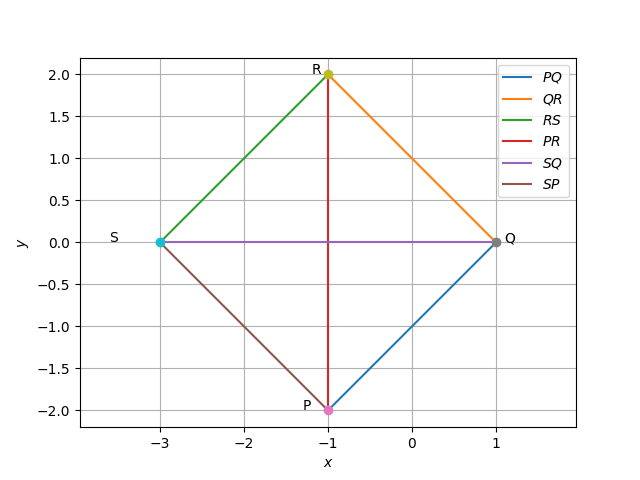
\includegraphics[width=\columnwidth]{./figs/vectors/quad1.png}
	\caption{quadrilateral1 }
	\label{fig:3.5.4_quadrilateral1}
\end{figure}
\begin{lstlisting}
codes/vectors/quad1.py
\end{lstlisting}

\item In Fig. 	\ref{fig:3.5.4_quadrilateral2}

\begin{align}
\vec{Q} - \vec{P} &= \myvec{6\\-4}
\\
\vec{R} - \vec{P} &= \myvec{3\\-2}
\\
\vec{Q} - \vec{R} &= \myvec{3\\-2}
\\
\left(\vec{Q} - \vec{P}\right) &= \left(\vec{R} - \vec{P}\right) + \left(\vec{Q} - \vec{R}\right) = \myvec{6\\-4}
\end{align}
Hence,  $\vec P,\vec Q$ and $\vec R$ lie on a straight line, so $PQRS$ is not  a quadrilateral.
%
\begin{figure}[!ht]
	\centering
	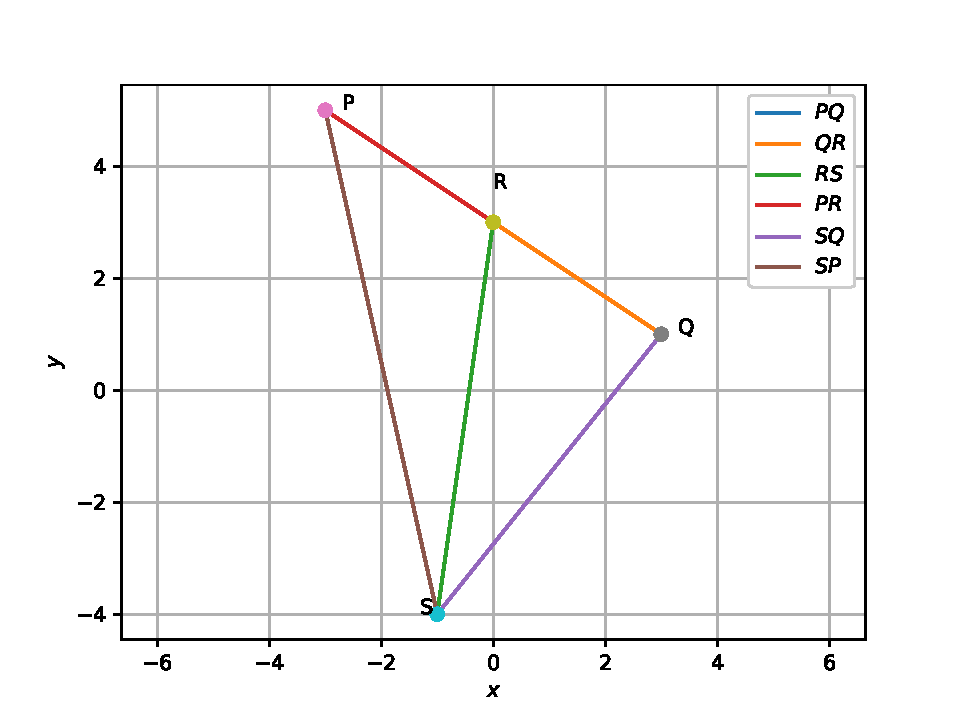
\includegraphics[width=\columnwidth]{./figs/vectors/quad2.pdf}
	\caption{quadrilateral2 }
	\label{fig:3.5.4_quadrilateral2}
\end{figure}
%
\item See Fig. 	\ref{fig:3.5.4_quadrilateral3}.

\begin{align}
\because \left(\vec{Q} - \vec{P}\right) &= \left(\vec{R} - \vec{S}\right) = \myvec{3\\1}
\\
\left(\vec{P} - \vec{S}\right) &= \left(\vec{Q} - \vec{R}\right) = \myvec{3\\3},
\end{align}
$PQRS$ is a parallelogram.  Also, 
%
\begin{align}
\norm{\vec{Q} - \vec{P}} \ne \norm{\vec{P} - \vec{S}}
\end{align}
Hence, $PQRS$ is neither a rhombus nor a square.
\begin{align}
\because \left(\vec{Q} - \vec{P}\right)^T \left(\vec{Q} - \vec{R}\right) = \myvec{3 & 1}\myvec{3\\3} \ne 0,
\end{align}
$PQRS$ is not a rectangle. 
%
\begin{figure}[!ht]
	\centering
	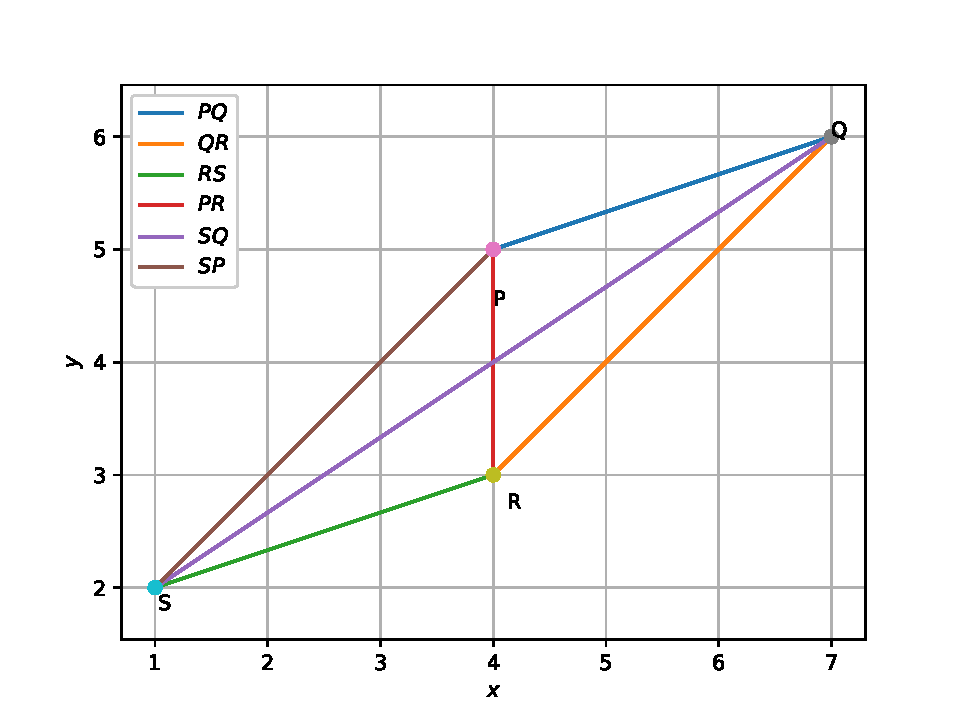
\includegraphics[width=\columnwidth]{./figs/vectors/quad3.pdf}
	\caption{}
	\label{fig:3.5.4_quadrilateral3}
\end{figure}

\end{enumerate}


\end{enumerate}

\subsection{Triangle}
\renewcommand{\theequation}{\theenumi}
\begin{enumerate}[label=\thesubsection.\arabic*.,ref=\thesubsection.\theenumi]
%\begin{enumerate}[label=\arabic*.,ref=\thesection.\theenumi]
\numberwithin{equation}{enumi}

%
\item Draw Fig. \ref{fig:tri_right_angle} for $a = 4, c =3$.
\label{const:tri_right_angle}
%
\begin{figure}[!ht]
\centering
\resizebox{\columnwidth}{!}{%Code by GVV Sharma
%December 6, 2019
%released under GNU GPL
%Drawing a right angled triangle

\begin{tikzpicture}[scale=2]

%Triangle sides
\def\a{4}
\def\c{3}

%Marking coordiantes
\coordinate [label=above:$A$] (A) at (0,\c);
\coordinate [label=left:$B$] (B) at (0,0);
\coordinate [label=right:$C$] (C) at (\a,0);

%Drawing triangle ABC
\draw (A) -- node[left] {$\textrm{c}$} (B) -- node[below] {$\textrm{a}$} (C) -- node[above,,xshift=2mm] {$\textrm{b}$} (A);

%Drawing and marking angles
\tkzMarkAngle[fill=orange!40,size=0.5cm,mark=](A,C,B)
\tkzMarkRightAngle[fill=blue!20,size=.3](A,B,C)
\tkzLabelAngle[pos=0.65](A,C,B){$\theta$}
\end{tikzpicture}
}
\caption{Right Angled Triangle}
\label{fig:tri_right_angle}	
\end{figure}
\\
\solution The vertices of $\triangle ABC$ are 
\begin{align}
\vec{A} = \myvec{0\\c} = \myvec{0\\3}, \vec{B} = \myvec{0\\0}, \vec{C} = \myvec{a\\0}=\myvec{4\\0}
\end{align}
%
The python code for  Fig. \ref{fig:tri_right_angle} is
\begin{lstlisting}
codes/triangle/tri_right_angle.py
\end{lstlisting}
%
and the equivalent latex-tikz code is
%
\begin{lstlisting}
figs/constr/triangle/tri_right_angle.tex
\end{lstlisting}
%
The above latex code can be compiled as a standalone document as
%
\begin{lstlisting}
figs/constr/triangle/tri_right_angle_alone.tex
\end{lstlisting}
%

\item Draw Fig. \ref{fig:tri_polar} for $a = 4, c =3$.
\label{const:tri_polar}
%
\\
\solution 
 The vertex  $\vec{A}$ can  be expressed  in {\em polar coordinate form} as
%\label{prob:tri_polar}
%
\begin{align}
\vec{A} = b\myvec{\cos \theta\\  \sin \theta} 
\end{align}
%
where
\begin{align}
b = \sqrt{a^2+c^2} = 5, \tan \theta = \frac{3}{4}
\end{align}
%The vertices of $\triangle ABC$ are 
%\begin{align}
%\vec{A} = \myvec{a\\c} = \myvec{4\\3}, \vec{B} = \myvec{a\\0}  = \myvec{4\\0}, \vec{C} = \myvec{0\\0}.
%\end{align}
%
The python code for  Fig. \ref{fig:tri_polar} is
\begin{lstlisting}
codes/triangle/tri_polar.py
\end{lstlisting}
%
and the equivalent latex-tikz code is
%
\begin{lstlisting}
figs/constr/triangle/tri_polar.tex
\end{lstlisting}
\begin{figure}[!ht]
\centering
\resizebox{\columnwidth}{!}{%Code by GVV Sharma
%December 6, 2019
%released under GNU GPL
%Drawing a right angled triangle

\begin{tikzpicture}[scale=2]

%Triangle sides
\def\a{4}
\def\c{3}

%Marking coordiantes
\coordinate [label=above:$A$] (A) at (\a,\c);
\coordinate [label=below:$B$] (B) at (\a,0);
\coordinate [label=left:$C$] (C) at (0,0);

%Drawing triangle ABC
\draw (A) -- node[left] {$\textrm{c}$} (B) -- node[below] {$\textrm{a}$} (C) -- node[above left,xshift=2mm] {$\textrm{b}$} (A);

%Drawing and marking angles
\tkzMarkAngle[fill=orange!40,size=0.5cm,mark=](B,C,A)
\tkzMarkRightAngle[fill=blue!20,size=.3](A,B,C)
\tkzLabelAngle[pos=0.65](A,C,B){$\theta$}
\end{tikzpicture}
}
\caption{Right Angled Triangle}
\label{fig:tri_polar}	
\end{figure}
%
\item Draw Fig. \ref{fig:tri_sss} with $a=6$, $b=5$  and $c=4$.  
\label{const:tri_sss}
\begin{figure}[!ht]
	\begin{center}
			\resizebox{\columnwidth}{!}{%Code by GVV Sharma
%December 7, 2019
%released under GNU GPL
%Drawing a triangle given 3 sides

\begin{tikzpicture}
[scale=2,>=stealth,point/.style={draw,circle,fill = black,inner sep=0.5pt},]

%Triangle sides
\def\a{6}
\def\b{5}
\def\c{4}
 
%Coordinates of A
%\def\p{{\a^2+\c^2-\b^2}/{(2*\a)}}
\def\p{2.25}
\def\q{{sqrt(\c^2-\p^2)}}

%Labeling points
\node (A) at (\p,\q)[point,label=above right:$A$] {};
\node (B) at (0, 0)[point,label=below left:$B$] {};
\node (C) at (\a, 0)[point,label=below right:$C$] {};

%Foot of perpendicular

\node (D) at (\p,0)[point,label=above right:$D$] {};

%Drawing triangle ABC
\draw (A) -- node[left] {$\textrm{c}$} (B) -- node[below] {$\textrm{a}$} (C) -- node[above,xshift=2mm] {$\textrm{b}$} (A);

%Drawing altitude AD
\draw (A) -- node[left] {$\textrm{h}$}(D);

%Drawing and marking angles
%\tkzMarkAngle[fill=orange!40,size=0.5cm,mark=](A,C,B)
%\tkzMarkAngle[fill=orange!40,size=0.4cm,mark=](D,B,A)
%\tkzMarkAngle[fill=green!40,size=0.5cm,mark=](B,A,C)
%\tkzMarkAngle[fill=green!40,size=0.5cm,mark=](C,B,D)
\tkzMarkRightAngle[fill=blue!20,size=.2](A,D,B)
%\tkzMarkRightAngle[fill=blue!20,size=.2](B,D,A)
%\tkzLabelAngle[pos=0.65](A,C,B){$\theta$}
%\tkzLabelAngle[pos=0.65](A,B,D){$\theta$}
%\tkzLabelAngle[pos=1](B,A,C){\rotatebox{-45}{$\alpha = 90\degree -\theta$}}
%\tkzLabelAngle[pos=0.65](C,B,D){$\alpha$}

\end{tikzpicture}
}
	\end{center}
	\caption{}
	\label{fig:tri_sss}	
\end{figure}
\\
\solution Let the vertices of  $\triangle ABC$ and $\vec{D}$ be 
\begin{align}
\label{eq:tri_basic}
\vec{A} = \myvec{p\\q}, \vec{B} = \myvec{0\\0}, \vec{C} = \myvec{a\\0}, \vec{D} = \myvec{p\\0}
\end{align}
%

Then
\begin{align}
\label{eq:c_tricoord}
AB &= \norm{\vec{A}-\vec{B}}^2 = \norm{\vec{A}}^2  = c^2 \quad \because \vec{B} = \vec{0}
\\
\label{eq:a_tricoord}
BC &= \norm{\vec{C}-\vec{B}}^2 = \norm{\vec{C}}^2  = a^2
\\
AC &= \norm{\vec{A}-\vec{C}}^2 =    b^2
\label{eq:b_tricoord}
\end{align}
%
From \eqref{eq:b_tricoord},
\begin{align}
b^2 &=\norm{\vec{A}-\vec{C}}^2 = \norm{\vec{A}-\vec{C}}^T\norm{\vec{A}-\vec{C}}  
\\
&= \vec{A}^T\vec{A}+\vec{C}^T\vec{C}-\vec{A}^T\vec{C} - \vec{C}^T\vec{A} 
\\
&= \norm{\vec{A}}^2 + \norm{\vec{C}}^2 - 2\vec{A}^T\vec{C} \quad \brak{\because \vec{A}^T\vec{C} = \vec{C}^T\vec{A} } 
\label{eq:tri_const_norm_ac}
\\
&= a^2+c^2-2ap
\end{align}
%
yielding
\begin{align}
p&= \frac{a^2+c^2-b^2}{2a}
\end{align}
%
From \eqref{eq:c_tricoord}, 
\begin{align}
\norm{\vec{A}}^2 &= c^2 = p^2+q^2
\\
\implies q&= \pm \sqrt{c^2-p^2}
\end{align}
%
The python code for  Fig. \ref{fig:tri_sss} is
\begin{lstlisting}
codes/triangle/tri_sss.py
\end{lstlisting}
%
and the equivalent latex-tikz code is
%
\begin{lstlisting}
figs/constr/triangle/tri_sss.tex
\end{lstlisting}

\end{enumerate}


\subsection{Quadrilateral}
\begin{enumerate}[label=\thesection.\arabic*,ref=\thesection.\theenumi]
\numberwithin{equation}{enumi}
\numberwithin{figure}{enumi}
\numberwithin{table}{enumi}

\item $ABCD$ is a quadrilateral in which $AB = BC$ and $AD = CD$. Show that $BD$ bisects both the angles $ABC$ and $ADC$.
\item $O$ is a point in the interior of a square $ABCD$ suchthat $OAB$ is an equilateral triangle. Show that $\triangle  OCD$ is an isosceles triangle.
\item Show that in a quadrilateral $ABCD$, 
\begin{align}
     AB + BC + CD + DA  <  (BD + AC)
\end{align} 
\item Show that in a quadrilateral $ABCD$,
\begin{align}
 AB + BC + CD + DA  >   AC + BD
\end{align}
\item Line segment joining the mid-points $M$ and $N$ of parallel sides $AB$ and $DC$, respectively of a trapezium $ABCD$ is perpendicular to both the sides $AB$ and $DC$. Prove that $AD = BC$.
\item $ABCD$ is a quadrilateral such that diagonal $AC$ bisects the angles $A$ and $C$. Prove that $AB = AD$ and $CB = CD$.
\item $AB$ and $CD$ are the smallest and largest sides of a quadrilateral $ABCD$. Out of $\angle B$ and $\angle D$ decide which is greater.
\item $ABCD$ is quadrilateral such that $AB = AD$ and $CB = CD$. Prove that $AC$ is the perpendicular bisector of $BD$.
\item A point $\vec{E} $ is taken on the side $BC$ of a parallelogram ABCD.$AE$ and  $DC$ are produced to meet at $\vec{F}$.Prove that  $ar (ADF) = ar (ABFC)$.
\item The diagonals of a parallelogram ABCD intersect at a point $\vec{O}$.Through $\vec{O}$,a line is drawn to intersect $AD$ at $\vec{P}$ and $BC$ at $\vec{Q}$.Show that $PQ$ divides the parallelogram into two parts of equal area.
\item The medians $BE$ and $CF$ of a triangle ABC intersect at $\vec{G}$.Prove that the area of $ \triangle${GBC}= area of the quadrilateral AFGE.	
\item In Fig.\ref{fig:exemplar/9.9.4/9.24},$CD \parallel AE$  and $CY \parallel BA$.Prove that  $ar (CBX) =  ar (AXY)$
\begin{figure}[h]
	\centering
	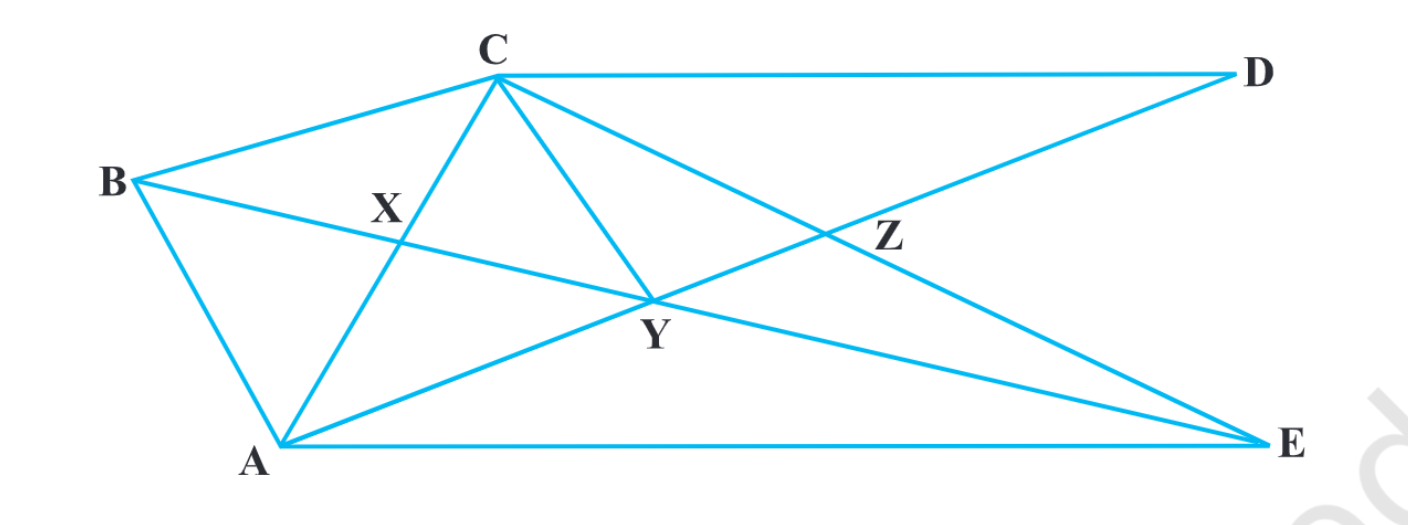
\includegraphics[width=\columnwidth]{exemplar/9.9.4/figs/Fig9.24.png}
	\caption{}
	\label{fig:exemplar/9.9.4/9.24}
\end{figure}
\item ABCD is a trapezium in which $AB \parallel DC$,$DC = 30cm$  and $AB = 50cm$.If $\vec{X}$ and $\vec{Y}$ are,respectively the mid-points of $AD$ and $BC$,prove that  $ar (DCYX) = \frac{7}{9} ar (XYBA)$.
\item  In $ \triangle${ABC},if $\vec{L}$ and $\vec{M}$ are the points on $AB$ and $AC$,respectively such that $LM \parallel BC$.Prove that $ar (LOB) = ar (MOC)$.
\item In Fig.\ref{fig:exemplar/9.9.4/9.25},ABCDE is any pentagon.$BP$ drawn parallel to $AC$ meets $DC$ produced at $\vec{P}$ and $EQ$ drawn parallel to $AD$ meets $CD$ produced at $\vec{Q}$.Prove that  $ ar (ABCDE) = ar (APQ) $.
\begin{figure}[h]
	\centering
	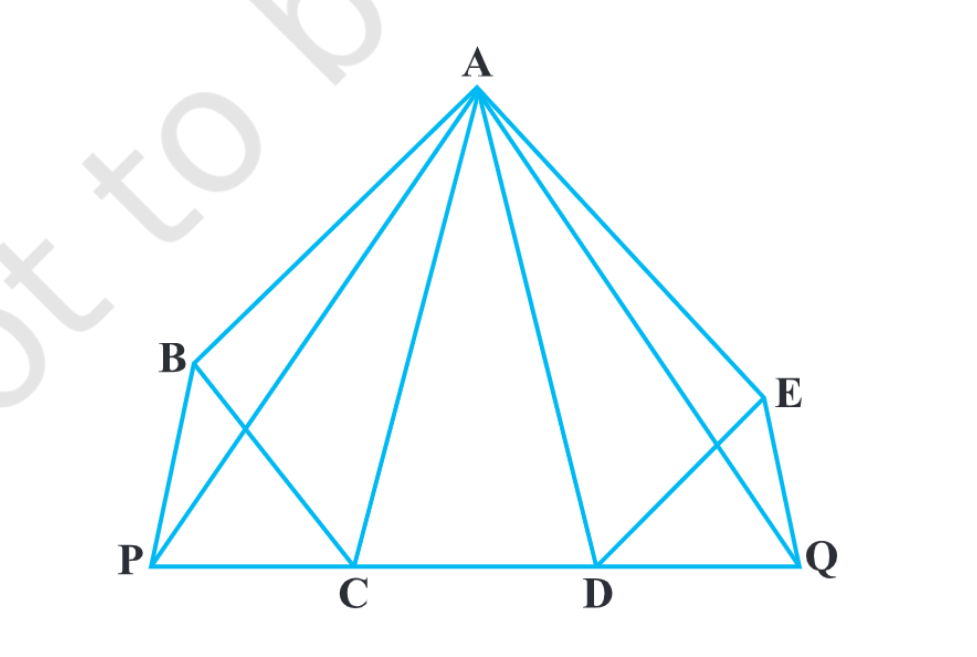
\includegraphics[width=\columnwidth]{exemplar/9.9.4/figs/Fig9.25.png}
	\caption{}
	\label{fig:exemplar/9.9.4/9.25}
\end{figure}
\item If the medians of a $ \triangle$ ABC  intersect at $\vec{G}$,show that
	\begin{align} 
		{ar (AGB)} &={ar (AGC)}= {ar (BGC)} = \frac{1}{3} {ar (ABC)}
	\end{align}
\item In Fig.\ref{fig:exemplar/9.9.4/9.26},$\vec{X}$ and $\vec{Y}$ are the mid-points of $AC$ and $AB$ respectively,$QP \parallel BC$ and $CYQ$ and $BXP$ are straight lines.Prove that $ ar (ABP) = ar (ACQ) $.
\begin{figure}[h]
	\centering
	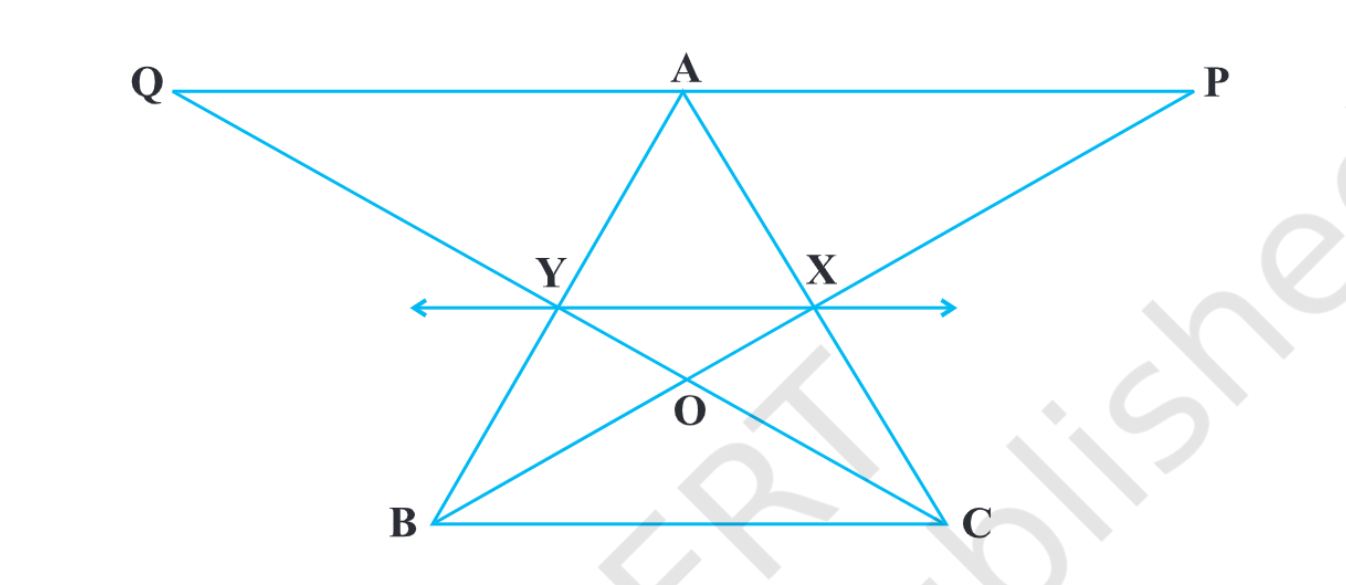
\includegraphics[width=\columnwidth]{exemplar/9.9.4/figs/Fig9.26.png}
	\caption{}
	\label{fig:exemplar/9.9.4/9.26}
\end{figure}
\item In Fig.\ref{fig:exemplar/9.9.4/9.27},ABCD and AEFD are two parallelograms.Prove that $ ar (PEA) = ar (QFD) $ [Hint:Join PD].
\begin{figure}[h]
	\centering
	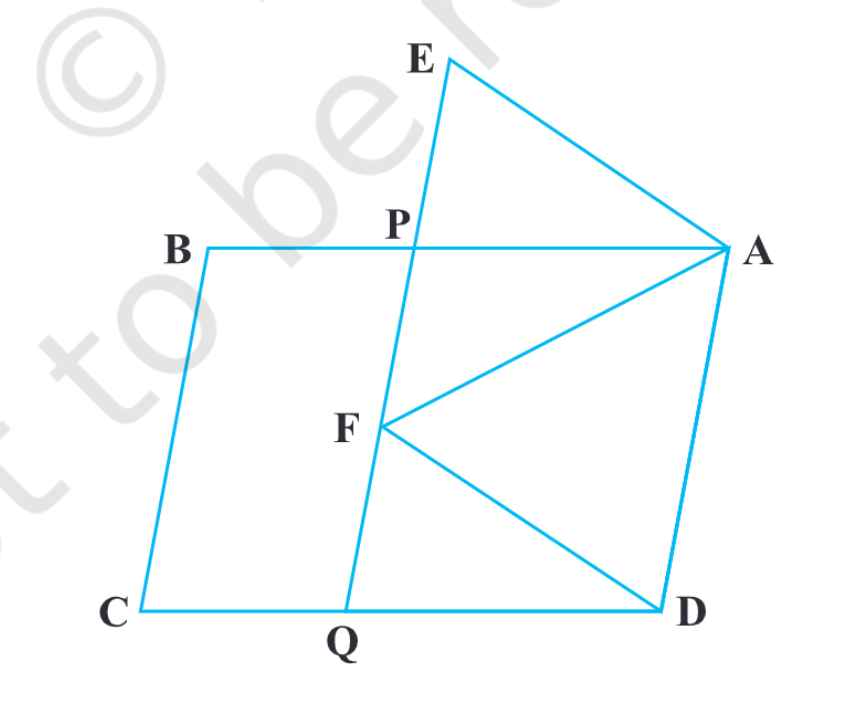
\includegraphics[width=\columnwidth]{exemplar/9.9.4/figs/Fig9.27.png}
	\caption{}
	\label{fig:exemplar/9.9.4/9.27}
\end{figure}
	\item ABCD is a parallelogram and $\vec{X}$ is the mid-point of AB.If $ ar(AXCD)= 24 cm^2 $ ,then $ar(ABC) =  24cm^2 $.
\item PQRS is a rectangle inscribed in a quadrant of radius 13 cm.A is any point on PQ.If PS=5 cm,then $ar(PAS)= 30 cm^2 $
\item PQRS is a parallelogram whose area is $ 180 cm^2 $ and A is any point on the diagonal QS.The area of $\triangle ASR =90 cm^2$.
\item ABC and BDE are two equilateral triangles such that $\vec{D}$is the mid-point of BC.Then ar(BDE)=$\frac{1}{4}  ar(ABC)$.
\item In Fig.\ref{fig:exemplar/9.8/9.8}, $ABCD$ and $EFGD$ are two parallelograms and $\vec{G}$ is the mid-point of $CD$. Then$ ar(DPC)=\frac{1}{2}  ar(EFGD)$.
	\begin{figure}[h]
		\centering
		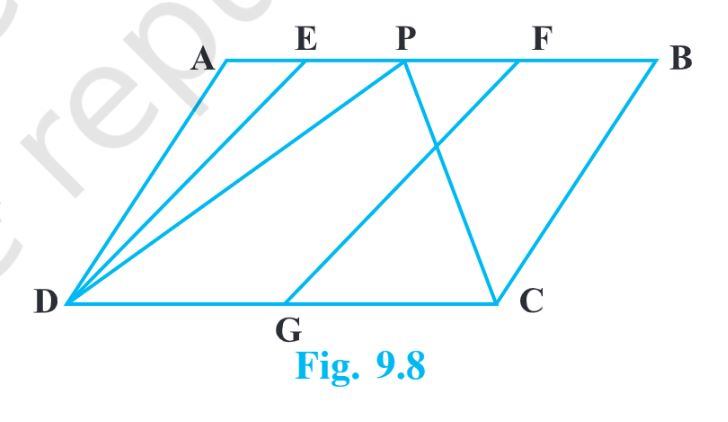
\includegraphics[width=\columnwidth]{exemplar/9.9.2/figs/9.8.jpg}
		\caption{}
		\label{fig:exemplar/9.8/9.8}
	\end{figure}
\item Construct a square of side $3 cm$.
\item Construct  a rectangle whose adjacent sides are of lengths $5 cm$ and $3.5 cm$.
\item Construct a rhombus whose side is of length $3.4 cm$ and one of its angles is $45\degree$.
\item Construct a rhombus whose diagonals are 4 cm and 6 cm in lengths.
\end{enumerate}

\subsection{Circle}
\iffalse
\documentclass[12pt]{article}
\usepackage{graphicx}
%\documentclass[journal,12pt,twocolumn]{IEEEtran}
\usepackage[none]{hyphenat}
\usepackage{graphicx}
\usepackage{listings}
\usepackage[english]{babel}
\usepackage{graphicx}
\usepackage{caption} 
\usepackage{hyperref}
\usepackage{booktabs}
\usepackage{commath}
\usepackage{gensymb}
\usepackage{array}
\usepackage{amsmath}   % for having text in math mode
\usepackage{listings}
\lstset{
  frame=single,
  breaklines=true
}
  
%Following 2 lines were added to remove the blank page at the beginning
\usepackage{atbegshi}% http://ctan.org/pkg/atbegshi
\AtBeginDocument{\AtBeginShipoutNext{\AtBeginShipoutDiscard}}
%


%New macro definitions
\newcommand{\mydet}[1]{\ensuremath{\begin{vmatrix}#1\end{vmatrix}}}
\providecommand{\brak}[1]{\ensuremath{\left(#1\right)}}
\providecommand{\norm}[1]{\left\lVert#1\right\rVert}
\newcommand{\solution}{\noindent \textbf{Solution: }}
\newcommand{\myvec}[1]{\ensuremath{\begin{pmatrix}#1\end{pmatrix}}}
\let\vec\mathbf
\begin{document}
\begin{center}
\title{\textbf{Circles}}
\date{\vspace{-5ex}} %Not to print date automatically
\maketitle
\end{center}
\setcounter{page}{1}
\section{11$^{th}$ Maths - Exercise 11.1.9}

\begin{enumerate}
\item Find the centre and radius of the given circle $2x^2+2y^2-x=0$
\section{Solution}
\fi
The given equation can be expressed as 
\begin{align}
	x^2+y^2-\frac{x}{2}&=0
	\\
\implies 	\norm{\vec{x}}^2+2\myvec{\frac{-1}{4} & 0}\vec{x}&=0
\end{align}	
The centre of circle is then given by 
\begin{align}
	\vec{u} = -\vec{c} 
=\myvec{\frac{1}{4}\\0}
\end{align}
and the radius of circle is obtained as
\begin{align}
	r=\sqrt{\norm{\vec{u}}^2 -f}
=\frac{1}{4}
\end{align}
See Fig. 
  \ref{fig:chapters/11/11/1/9/Figure}.
\begin{figure}[h]
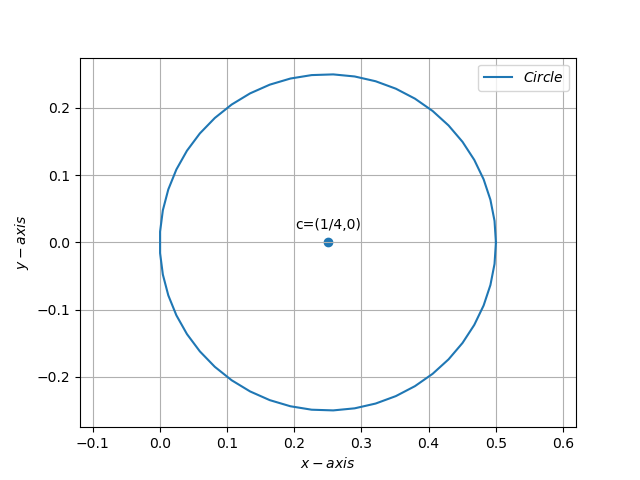
\includegraphics[width=\columnwidth]{chapters/11/11/1/9/figs/fig.png}
\caption{}
  \label{fig:chapters/11/11/1/9/Figure}
\end{figure}

%
\subsection{Vector Calculus}
\renewcommand{\theequation}{\theenumi}
\begin{enumerate}[label=\thesubsection.\arabic*.,ref=\thesubsection.\theenumi]
\numberwithin{equation}{enumi}
\item {\em Definition: }Let $\vec{x} \in \mathbb{R}^2, f\brak{\vec{x}} \in \mathbb{R}$.  Then, 
\begin{align}
\frac{df\brak{\vec{x}}}{d\vec{x}} = \myvec{\frac{\partial f(\vec{x})}{\partial x_1}\\\frac{\partial f(\vec{x})}{\partial x_2}}
\end{align}
\item 
\begin{align}
\begin{split}
\frac{d\vec{x}}{dx_1} &= \myvec{\frac{dx_1}{dx_1} \\ \frac{dx_1}{dx_1}} 
\\
&= \myvec{1\\m} = \vec{m}
\end{split}
\label{eq:calc_m_diff}
\end{align}
\item Show that 
\begin{align}
\begin{split}
\frac{d\brak{\vec{u}^T\vec{x}}}{d\vec{x}} &= \vec{u}
\\
\frac{d\brak{\vec{x}^T\vec{V}\vec{x}}}{d\vec{x}} &= 2\vec{V}^T\vec{x}
\end{split}
\label{eq:calc_vec_diff}
\end{align}
\item Differentiating \eqref{eq:conic_quad_form}
%\eqref{eq:ellipse_vec}  
with respect to $x_1$,
%
%\numberwithin{equation}{enumi}
\begin{align}
\label{eq:ellipse_tangent_der}
\sbrak{\frac{d\brak{\vec{x}^T\vec{V}\vec{x}}}{d\vec{x}}}^T\frac{d\vec{x}}{dx_1}
+2\frac{d\brak{\vec{u}^T\vec{x}}}{\vec{x}} \frac{d\vec{x}}{dx_1}
= 0
\\
\implies 2\brak{\vec{V}^T\vec{x}+\vec{u}}\vec{m}  = 0  
\end{align}
from \eqref{eq:calc_m_diff} and \eqref{eq:calc_vec_diff}.
%
%and \eqref{eq:ellipse_vec_diff}.
Substituting  the point of contact $\vec{x} = \vec{q}$ and simplifying results in
\begin{align}
\brak{\vec{V}\vec{q}+\vec{u}}\vec{m} & = 0 
\label{eq:ellipse_tangent_der_std}
\end{align}
%
which, upon taking the transpose, yields 
\eqref{eq:conic_tangent_mq}.
\end{enumerate}

\subsection{Vector Inequalities}
\renewcommand{\theequation}{\theenumi}
\begin{enumerate}[label=\thesubsection.\arabic*.,ref=\thesubsection.\theenumi]
\numberwithin{equation}{enumi}
\item {\em  (Cauchy-Schwarz Inequality:)} Show that 
%
\begin{align}
\abs{\vec{a}^T\vec{b}} \le \norm{\vec{a}}\norm{\vec{b}}
\end{align}
\proof  Using the definition of the inner product,
\begin{align}
\cos \theta = \frac{\vec{a}^T\vec{b}} {\norm{\vec{a}}\norm{\vec{b}}} 
\\
\because \abs{\cos \theta} \le 1, 
\abs{\vec{a}^T\vec{b}} \le \norm{\vec{a}}\norm{\vec{b}}
\end{align}
\item {\em (Triangle Inequality:)} Show that 
%
\begin{align}
\norm{\vec{a}+\vec{b}} \le \norm{\vec{a}}+\norm{\vec{b}}
\end{align}
\proof Let $\vec{O}$ be the origin.  In the triangle formed by $\vec{O}, \vec{a}$ and $-\vec{b}$, the lengths of the sides are
%
\begin{align}
\norm{\vec{a}}, 
\norm{\vec{b}}, 
\norm{\vec{a}+\vec{b}} 
\end{align}
%
$\because $ the sum of two sides of a triangle is always greater than the third side, 
\begin{align}
\norm{\vec{a}+\vec{b}} \le \norm{\vec{a}} + \norm{\vec{b}}
\end{align}

\end{enumerate}

%
\section{Linear Forms}
\subsection{Line}
\iffalse
\documentclass[journal,12pt,twocolumn]{article}
\usepackage{graphicx}
\graphicspath{{./figs/}}{}
\usepackage{amsmath,amssymb,amsfonts,amsthm}
\newcommand{\myvec}[1]{\ensuremath{\begin{pmatrix}#1\end{pmatrix}}}
\let\vec\mathbf
\title{
Matrix-Lines
}
\author{SHREYASH CHANDRA PUTTA}
\begin{document}
\maketitle
\tableofcontents

\section{Problem Statement}
\fi
A line perpendicular to the line segement joining the points (1,0) and (2,3) divides it in the ratio $1:n$. Find the equation of the line.
	\begin{figure}[!ht]
		\centering
 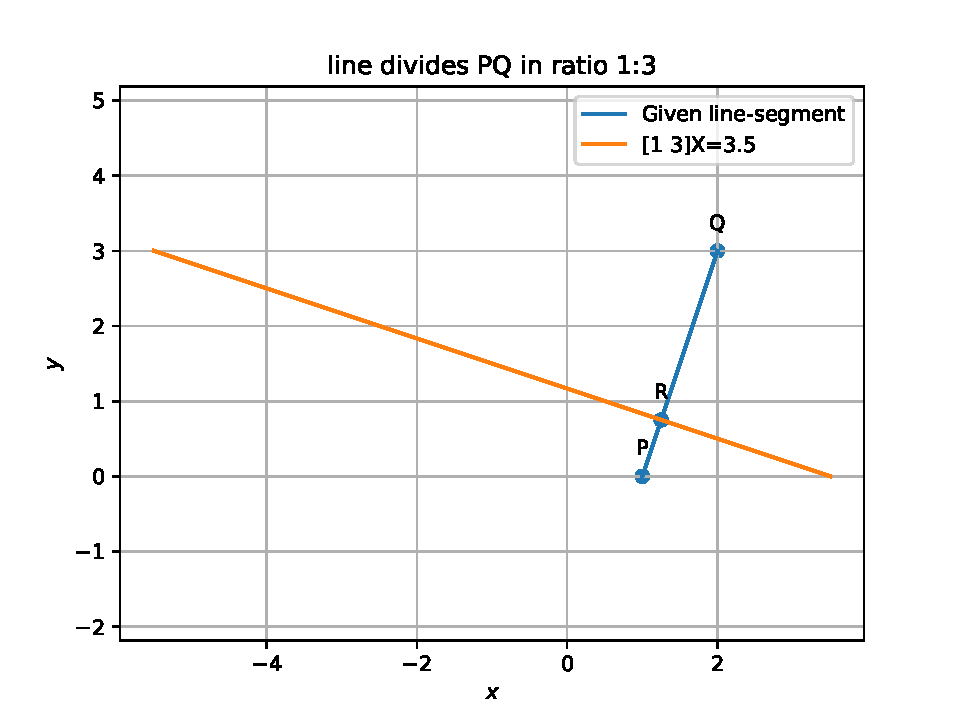
\includegraphics[width=\columnwidth]{chapters/11/10/2/11/figs/linefig.pdf}
		\caption{}
		\label{fig:11/10/2/11}
  	\end{figure}
	\\
	\solution 
\iffalse
(note: we are taking n as user Input) .

% 

\begin{table}[h]
    \centering
    \begin{tabular}{|c|c|c|}
       \hline
       \textbf{Symbol}&\textbf{Value}&\textbf{Description}  \\
       \hline
	    $\vec{P}$ & $\myvec{
		    1\\
		    0}$
	    & given point\\
        \hline
	    $\vec{Q}$ & $\myvec{2\\3}$
 & given point\\
        \hline
	    $\vec{R}$ & $\myvec{
  \frac{2+n}{1+n}\\
  \frac{3}{1+n}}$
 & intersecting point  \\
       \hline
    \end{tabular}
    \caption{Parameters}
    \label{tab:my_label}
\end{table}

%\section{Construction}

\begin{figure}[h]
    \centering
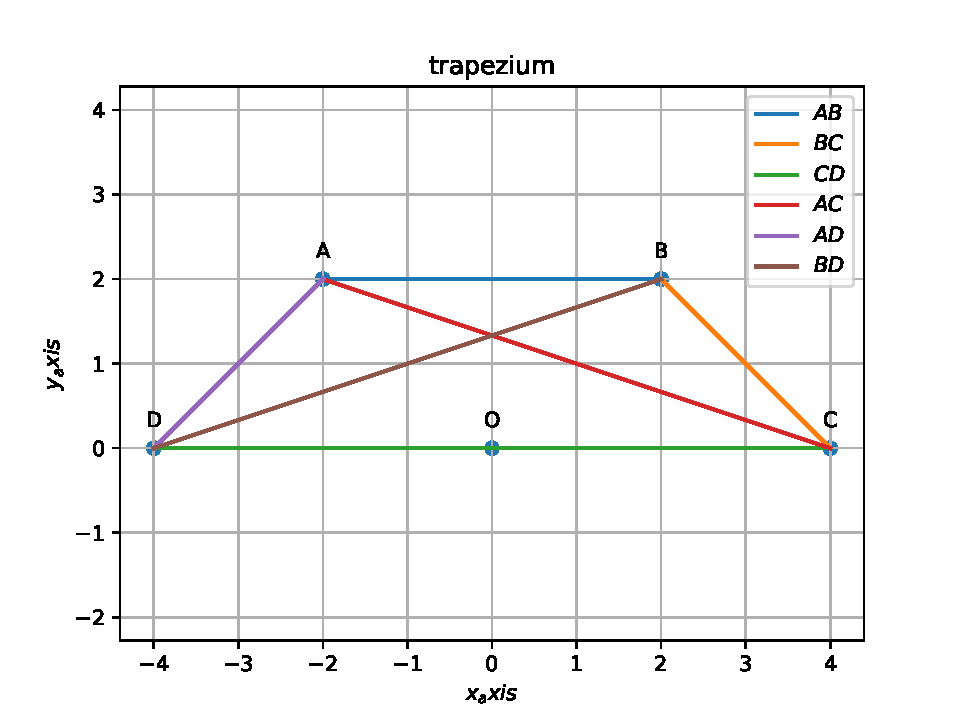
\includegraphics[width=\columnwidth]{fig/linefig.pdf}
    \caption{Equation of the required Straight Line}
    \label{fig:my_label}
\end{figure}




\section{Solution}

Given that resultant will divide the equation of line in the ratio 1:n and the line is perpendicular to line segment joining the points (1,0)and(2,3)  ) \\
%so, b = 9 - a  \\
\\
\fi 
Let 
\begin{align}
{\vec{P}}=\myvec{
  1\\
  0},
 {\vec{Q}}=\myvec{
  2\\
  3}
\end{align}
\iffalse
%	\vec{n^{\top}}
%	\myvec{
 % a\\
  %0}
  %= c \label{eq-1}
%\end{align}
\\
\fi
The direction vector of 
$PQ$ is 
\begin{align}
	\vec{m}=
     \vec{Q
 }-  \vec{P
 }
=
     \myvec{
  1\\
  3
 }
\end{align}
\iffalse
\\
We know, that position or  directional vector of points P and Q line segement used as the normal vector
\\
\\
 The general equation of the required perpendicular line is
 ${\vec{M^{\top}}\vec{X}} = c$.
 \\
 \\
 The perpendicular line cutting a line segment P and Q in ratio 1:n is passes through the point R.
 \fi
 Also, using section formula, 
 \begin{align}
	 \vec{R}=\frac{\vec{Q}+n\vec{P}}{1+n}
\end{align}
and the 
equation of line passing through ${\vec{R}}$ is
\begin{align}
	\vec{m}^{\top}\brak{\vec{x}-\vec{R}}=0
\\
\implies 
	   \myvec{
		   1 &  3}\vec{x}
	   &= \myvec{
  1\ 3}\myvec{
  \frac{2+n}{1+n}\\
  \frac{3}{1+n}} 
  \\
	&=	  \frac{11+n}{1+n} 
\end{align}
\iffalse



 
\section{Software}
Download the following code using,
\begin{table}[h]
    \centering
    \begin{tabular}{|c|}
    \hline \\
         svn co https://github.com/chanduputta/ \\FWC-Module1Assignments/blob/\\main/assignment4/line/lines3.py  \\
         \\
\hline
    \end{tabular}
\end{table}
\\
and execute the code by using command
\begin{center}
	\textbf{cmd:}
{Python3  lines3.py}\\
	\textbf{Then,}
{input your required n value}
\end{center}

\section{Conclusion}
\begin{center}
We found the equation of a line perpendicular to the line segement joining the points (1,0)and(2,3) divides it in the ratio 1:n .
\end{center}
\end{document}
\fi

\subsection{Plane}
\iffalse
\documentclass[journal,12pt,twocolumn]{IEEEtran}
\usepackage{setspace}
\usepackage{gensymb}
\usepackage{xcolor}
\usepackage{caption}
\singlespacing
\usepackage{siunitx}
\usepackage[cmex10]{amsmath}
\usepackage{mathtools}
\usepackage{hyperref}
\usepackage{amsthm}
\usepackage{mathrsfs}
\usepackage{txfonts}
\usepackage{stfloats}
\usepackage{cite}
\usepackage{cases}
\usepackage{subfig}
\usepackage{longtable}
\usepackage{multirow}
\usepackage{enumitem}
\usepackage{bm}
\usepackage{mathtools}
\usepackage{listings}
\usepackage{tikz}
\usetikzlibrary{shapes,arrows,positioning}
\usepackage{circuitikz}
\renewcommand{\vec}[1]{\boldsymbol{\mathbf{#1}}}
\DeclareMathOperator*{\Res}{Res}
\renewcommand\thesection{\arabic{section}}
\renewcommand\thesubsection{\thesection.\arabic{subsection}}
\renewcommand\thesubsubsection{\thesubsection.\arabic{subsubsection}}

\renewcommand\thesectiondis{\arabic{section}}
\renewcommand\thesubsectiondis{\thesectiondis.\arabic{subsection}}
\renewcommand\thesubsubsectiondis{\thesubsectiondis.\arabic{subsubsection}}
\hyphenation{op-tical net-works semi-conduc-tor}

\lstset{
language=Python,
frame=single, 
breaklines=true,
columns=fullflexible
}
\begin{document}
\theoremstyle{definition}
\newtheorem{theorem}{Theorem}[section]
\newtheorem{problem}{Problem}
\newtheorem{proposition}{Proposition}[section]
\newtheorem{lemma}{Lemma}[section]
\newtheorem{corollary}[theorem]{Corollary}
\newtheorem{example}{Example}[section]
\newtheorem{definition}{Definition}[section]
\newcommand{\BEQA}{\begin{eqnarray}}
        \newcommand{\EEQA}{\end{eqnarray}}
\newcommand{\define}{\stackrel{\triangle}{=}}
\newcommand{\myvec}[1]{\ensuremath{\begin{pmatrix}#1\end{pmatrix}}}
\newcommand{\mydet}[1]{\ensuremath{\begin{vmatrix}#1\end{vmatrix}}}
\bibliographystyle{IEEEtran}
\providecommand{\nCr}[2]{\,^{#1}C_{#2}} % nCr
\providecommand{\nPr}[2]{\,^{#1}P_{#2}} % nPr
\providecommand{\mbf}{\mathbf}
\providecommand{\pr}[1]{\ensuremath{\Pr\left(#1\right)}}
\providecommand{\qfunc}[1]{\ensuremath{Q\left(#1\right)}}
\providecommand{\sbrak}[1]{\ensuremath{{}\left[#1\right]}}
\providecommand{\lsbrak}[1]{\ensuremath{{}\left[#1\right.}}
\providecommand{\rsbrak}[1]{\ensuremath{{}\left.#1\right]}}
\providecommand{\brak}[1]{\ensuremath{\left(#1\right)}}
\providecommand{\lbrak}[1]{\ensuremath{\left(#1\right.}}
\providecommand{\rbrak}[1]{\ensuremath{\left.#1\right)}}
\providecommand{\cbrak}[1]{\ensuremath{\left\{#1\right\}}}
\providecommand{\lcbrak}[1]{\ensuremath{\left\{#1\right.}}
\providecommand{\rcbrak}[1]{\ensuremath{\left.#1\right\}}}
\theoremstyle{remark}
\newtheorem{rem}{Remark}
\newcommand{\sgn}{\mathop{\mathrm{sgn}}}
\newcommand{\rect}{\mathop{\mathrm{rect}}}
\newcommand{\sinc}{\mathop{\mathrm{sinc}}}
\providecommand{\abs}[1]{\left\vert#1\right\vert}
\providecommand{\res}[1]{\Res\displaylimits_{#1}}
\providecommand{\norm}[1]{\lVert#1\rVert}
\providecommand{\mtx}[1]{\mathbf{#1}}
\providecommand{\mean}[1]{E\left[ #1 \right]}
\providecommand{\fourier}{\overset{\mathcal{F}}{ \rightleftharpoons}}
\providecommand{\ztrans}{\overset{\mathcal{Z}}{ \rightleftharpoons}}
\providecommand{\system}[1]{\overset{\mathcal{#1}}{ \longleftrightarrow}}
\newcommand{\solution}{\noindent \textbf{Solution: }}
\providecommand{\dec}[2]{\ensuremath{\overset{#1}{\underset{#2}{\gtrless}}}}
\let\StandardTheFigure\thefigure
\def\putbox#1#2#3{\makebox[0in][l]{\makebox[#1][l]{}\raisebox{\baselineskip}[0in][0in]{\raisebox{#2}[0in][0in]{#3}}}}
\def\rightbox#1{\makebox[0in][r]{#1}}
\def\centbox#1{\makebox[0in]{#1}}
\def\topbox#1{\raisebox{-\baselineskip}[0in][0in]{#1}}
\def\midbox#1{\raisebox{-0.5\baselineskip}[0in][0in]{#1}}

\vspace{3cm}
\title{12.11.3.9}
\author{Lokesh Surana}
\maketitle
\section*{Class 12, Chapter 11, Exercise 3.9}


\solution The equation of given are given by
\begin{align}
	 {P}_1: \vec{n}_1^{\top}{\vec{x}} &= {c}_1\\
	 {P}_1: \vec{n}_1^{\top}{\vec{x}} &= {c}_2
\end{align}
%
\fi
The parameters of the given planes are
\begin{align}
 \vec{n}_1 = \myvec{3\\-1\\2},\,
 \vec{n}_1 = \myvec{1\\1\\1},\,
	c_1 = 4, c_2 = 2.
\end{align}
The intersection of the planes is given as
\begin{align}
\vec{n}_1^{\top}{\vec{x}} - {c}_1 + \lambda\brak{\vec{n}_2^{\top}{\vec{x}} - {c}_2} &= 0
\end{align}
where 
\begin{align}
	\lambda = \frac{{c}_1 - {n}_1^{\top}\vec{P}}{{n}_2^{\top}\vec{P} - {c}_2} 
= -\frac{2}{3}  
\end{align}
upon substituting 
\begin{align}
\vec{P} = \myvec{2\\2\\1}
\end{align}
Thus, 
the equation of plane is 
\begin{align}
 \myvec{7&-5&4}\vec{x} = 8
\end{align}


\subsection{Pseudo Inverse}
\renewcommand{\theequation}{\theenumi}
\begin{enumerate}[label=\thesubsection.\arabic*.,ref=\thesubsection.\theenumi]
\numberwithin{equation}{enumi}

\item To find the shortest distance between the lines 
\begin{align}
    L_1\colon \vec{x}=\myvec{1\\2\\1}+\lambda_1\myvec{1\\-1\\1}\label{eq:pseudo:1}\\
    L_2\colon \vec{x}=\myvec{2\\-1\\-1}+\lambda_2\myvec{2\\1\\2}\label{eq:pseudo:2}
\end{align}
\item If the two lines intersect,
\begin{align}
\vec{x}_1 + \lambda_1 \vec{m}_1
=\vec{x}_2 + \lambda_2 \vec{m}_2
\\
\implies \myvec{\vec{m}_1 & \vec{m}_2}\myvec{\lambda_1 \\ -\lambda_2} = \vec{x}_2 - \vec{x}_1
\\
\text{or, } \vec{M}\myvec{\lambda_1 \\ -\lambda_2} = \vec{x}_2 - \vec{x}_1
\label{eq:pseudo_intersect}
\end{align}
%
where 
\begin{align}
\label{eq:pseudo_xm}
\vec{x}_1 = \myvec{1\\2\\1},
\vec{x}_2 = \myvec{2\\-1\\-1},
\vec{m}_1 = \myvec{1\\-1\\1},
\vec{m}_2 = \myvec{2\\1\\2}.
\\
\vec{M} =\myvec{\vec{m}_1 & \vec{m}_2}
\label{eq:pseudo_rect}
\end{align}
\eqref{eq:pseudo_intersect} can be expressed as the matrix equation 
\begin{align}
\myvec{
1 & 2
\\
-1 & 1
\\
1 & 2
}
\vec{x} =
\myvec{1 \\ -3 \\ -2}
\label{eq:pseudo_mat_eq}
\end{align}

From the augmented matrix in \eqref{eq:pseudo_intersect},
%
\begin{align}
%    \myvec{1\\2\\1}+\lambda_1\myvec{1\\-1\\1}=\myvec{2\\-1\\-1}+\lambda_2\myvec{2\\1\\2}\\
%    \lambda_1\myvec{1\\-1\\1}-\lambda_2\myvec{2\\1\\2}=\myvec{1\\-3\\-2}\\
%    \myvec{1 & -2\\-1 & -1\\1 & -2}\myvec{\lambda_1\\\lambda_2}=\myvec{1\\-3\\-2}\\
%    \intertext{The Augmented matrix will be}
    \myvec{1 & -2 & 1\\-1 & -1 & -3\\1 & -2 & -2}\\
    \myvec{1 & -2 & 1\\-1 & -1 & -3\\1 & -2 & -2}\xleftrightarrow{R_1=R_1-R_2}\myvec{0 & 0 & 3\\-1 & -1 & -3\\1 & -2 & -2}
\end{align}
The above matrix has a $rank=3$. Hence the lines do not intersect.
\item Let 
\begin{align}
\vec{A}=\vec{x}_1 + \lambda_1 \vec{m}_1
\\
\vec{B}=\vec{x}_2 + \lambda_2 \vec{m}_2
\label{eq:pseudo_AB}
\end{align}
be the closest points on $L_1$ and $L_2$ respectively.  Then the shortest distance between two skew lines 
will be the length of line perpendicular to both the lines $L_1$,$L_2$ and passing through $A$ and $B$.
Thus, 
\begin{align}
    \vec{m_1}^T\brak{\vec{A}-\vec{B}}=0\label{eq:pseudo:32}\\
    \vec{m_2}^T\brak{\vec{A}-\vec{B}}=0\label{eq:pseudo:34}\\
\implies \vec{M}^T\brak{\vec{A}-\vec{B}} = 0
\label{eq:pseudo:MAB}
\end{align}
From \eqref{eq:pseudo_AB} and \eqref{eq:pseudo_rect}
%
\begin{align}
    \vec{A-B}=\vec{x_1-x_2}+\vec{M}\myvec{\lambda_1\\ -\lambda_2}
\label{eq:pseudo:31}
\end{align}
and using \eqref{eq:pseudo:MAB}, in the above, 

%\begin{align}
%    \vec{m_1^T}(\vec{x_1-x_2})+\vec{m_1^T}(\vec{m_1} & -\vec{m_2})\begin{pmatrix}\lambda_1 \\ \lambda_2\end{pmatrix}=0\label{eq:33}
%\end{align}
%The dot product of $\vec{m_2}$ with the line ${AB}$ is
%\begin{align}
%    \vec{m_2}^T\brak{\vec{A-B}}=0\label{eq:34}\\
%    \vec{m_1^T}(\vec{x_1-x_2})+\vec{m_2^T}(\vec{m_1} & -\vec{m_2})\myvec{\lambda_1 \\ \lambda_2}=0\label{eq:35}
%\end{align}
%Let the matrix $\vec{M}$ be
%\begin{align}
%    \vec{M}=\myvec{\vec{m_1}^T\\\vec{m_2}^T}\label{eq:36}
%\end{align}
%Combining the equations \eqref{eq:33} and \eqref{eq:35} in matrix form,using equation \eqref{eq:36}, we get
\begin{align}
    \vec{M}^T\vec{M}\myvec{\lambda_1\\-\lambda_2} = \vec{M}^T\brak{\vec{x}_2-\vec{x}_1}
\label{eq:pseudo_ls}
\end{align}
%simplifying it further
%\begin{align}
%    \vec{M}\vec{M}^T\begin{pmatrix}\lambda_1\\-\lambda_2\end{pmatrix}=\vec{M}\vec{(x_2-x_1)}
%\end{align}
\item Substituting the values from \eqref{eq:pseudo_xm} in \eqref{eq:pseudo_ls} and forming the augmented matrix,
%To find the points on the lines which make up the shortest distance we need to find $\lambda_1$ and $\lambda_2$ using the above expression to get the augmented form
\begin{align}
%    \myvec{\vec{m_1}^T\vec{m_1} & \vec{m_1}^T\vec{m_2}\\\vec{m_2}^T\vec{m_1} & \vec{m_2}^T\vec{m_2}}\myvec{\lambda_1\\-\lambda_2}=\myvec{\vec{m_1}^T\vec{(x_2-x_1)}\\\vec{m_2}^T\vec{(x_2-x_1)}}\\
%    \myvec{\vec{m_1}^T\vec{m_1} & \vec{m_1}^T\vec{m_2} & \vec{m_1}^T\vec{(x_2-x_1)}\\\vec{m_2}^T\vec{m_1} & \vec{m_2}^T\vec{m_2} & \vec{m_2}^T\vec{(x_2-x_1)}}\\
%    \intertext{we know that}
%    \vec{x_1}=\myvec{1\\2\\1},\vec{x_2}=\myvec{2\\-1\\-1},\vec{m_1}=\myvec{1\\-1\\1} and  \vec{m_2}=\myvec{2\\1\\2}
%    \intertext{so the augmented matrix will be}
    \myvec{3 & 3 &2\\ 3 & 9 & -5}\\
    \myvec{3 & 3 &2\\ 3 & 9 & -5}\xleftrightarrow{R_2=R_2-R_1}\myvec{3 & 3 &2\\ 0 & 6 & -7}\\
    \myvec{3 & 3 &2\\ 0 & 6 & -7}\xleftrightarrow{R_1=2R_1-R_2}\myvec{6 & 0 & 11\\ 0 & 6 & -7}\\
    \myvec{6 & 0 & 11\\ 0 & 6 & -7}\xleftrightarrow{R_1=\frac{R_1}{6},R_2=\frac{R_2}{6}}\myvec{1 & 0 & \frac{11}{6}\\ 0 & 1 & \frac{-7}{6}}\\
    \lambda_1=\frac{11}{6},\lambda_2=\frac{7}{6}
\end{align}
yielding
\begin{align}
A=\frac{1}{6}\myvec{17\\1\\17},
B=\frac{1}{6}\myvec{26\\1\\8}. 
\end{align}
%
\item The distance is then obtained as
%The shortest distance between the lines is the distance between the points $A$ and $B$.
\begin{align}
    \norm{\vec{B}-\vec{A}} 
%    =\norm{\frac{1}{{6}}\myvec{17\\1\\17}-\frac{1}{{6}}\myvec{26\\1\\8}}\\
    =\frac{3}{\sqrt{2}}
\end{align}
%Therefore the shortest distance between the given lines is $\frac{3}{\sqrt{2}}$.\par
%
%The unit vector perpendicular to lines
%\begin{align}
%    Line_1\colon \vec{x}=\vec{x_1}+\lambda_1\vec{m_1}\\
%    Line_2\colon \vec{x}=\vec{x_2}+\lambda_1\vec{m_2}
%\end{align}
%can be found by 
%\begin{align}
%    \vec{n}=\frac{\vec{A-B}}{\norm{\vec{A-B}}}\\
%    \vec{n}=\frac{\frac{1}{{6}}\myvec{17\\1\\17}-\frac{1}{{6}}\myvec{26\\1\\8}}{\frac{3}{\sqrt{2}}}\\
%    \vec{n}=\frac{1}{\sqrt{2}}\begin{pmatrix}-1\\0\\1\end{pmatrix}
%\end{align}
%
%So the unit vector perpendicular to both $L_1$ and $L_2$ is
%\begin{align}
%    \vec{n}=\frac{1}{\sqrt{2}}\begin{pmatrix}-1\\0\\1\end{pmatrix}
%\end{align}
Fig.     \ref{fig:pseudo_Skew_lines} shows the various points and distances between the lines.
\begin{figure}[!ht]
\centering
    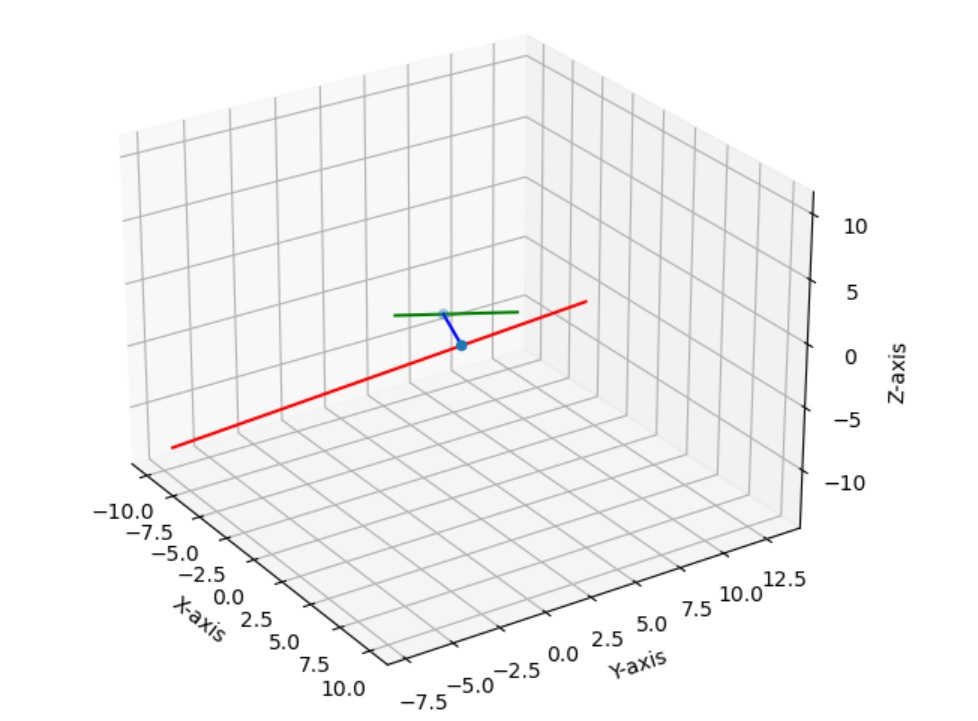
\includegraphics[width=\columnwidth]{./figs/pseudo/assignment2.jpg}
    \caption{This is the plot of the given skew lines and the blue line indicates the normal to the given lines}
    \label{fig:pseudo_Skew_lines}
\end{figure}


\end{enumerate}

\section{Quadratic Forms}
\subsection{Introduction}
\renewcommand{\theequation}{\theenumi}
\begin{enumerate}[label=\thesubsection.\arabic*.,ref=\thesubsection.\theenumi]
\numberwithin{equation}{enumi}
\item Let $\vec{P}$ be a point such that the ratio of its distance from a fixed point $\vec{F}$ and the distance ($d$) from a fixed line 
$L: \vec{n}^T\vec{x}=c$ is constant, given by 
\label{conics/30/def}
\begin{align}
\frac{\norm{\vec{P}-\vec{F}}}{d} = e    
\end{align}
The locus of $\vec{P}$ such is known as a conic section. The line $L$ is known as the directrix and the point $\vec{F}$ is the focus. $e$ is defined to be 
the eccentricity of the conic.  
\begin{enumerate}
    \item For $e = 1$, the conic is a parabola
    \item For $e < 1$, the conic is an ellipse
    \item For $e > 1$, the conic is a hyperbola
\end{enumerate}

% \item     
% \begin{definition}
% \end{definition}
\item 
%\begin{theorem}
The equation of  a conic is given by 
\begin{align}
    \label{eq:conic_quad_form}
    \vec{x}^T\vec{V}\vec{x}+2\vec{u}^T\vec{x}+f=0
    \end{align}
where     
\begin{align}
\vec{V} &= t\vec{I}-\vec{n}\vec{n}^T, 
\\
\vec{u} &= c\vec{n}-t\vec{F}, 
\\
f &= t\norm{\vec{F}}^2-c^2
    \end{align}
    
% \begin{align}
% \vec{x}^T(t\vec{I}-\vec{n}\vec{n}^T)\vec{x}+2(c\vec{n}-t\vec{F})^T\vec{x}+t\norm{\vec{F}}^2-c^2&=0
% \end{align}
%
and 
\begin{align}
    t=\frac{\norm{\vec{n}}^2}{e^2}
\end{align}
%\end{theorem}

\solution See Appendix \ref{app:conicdef}

% \item The general equation of second degree is given by
% \begin{align}
% ax^2+2bxy+cy^2+2dx+2ey+f=0
% \end{align}
% and can be expressed as
% \begin{align}
% \label{eq:conic_quad_form}
% \vec{x}^T\vec{V}\vec{x}+2\vec{u}^T\vec{x}+f=0
% \end{align}
% %
% where
% \begin{align}
% \vec{V} &= \vec{V}^T = \myvec{a & b \\ b & c}
% \\
% \vec{u} &= \myvec{d & e}
% \end{align}

\item {\em (Affine Transformation and Eigenvalue Decompostion)}
Using 
\begin{align}
\vec{x} = \vec{P}\vec{y}+\vec{c} \quad \text{(Affine Transformation)}
\label{eq:conic_affine}
\end{align}
such that 
\begin{align}
%\begin{split}
\label{eq:conic_parmas_eig_def}
\vec{P}^T\vec{V}\vec{P} &= \vec{D}. \quad \text{(Eigenvalue Decomposition)}
\\
\vec{D} &= \myvec{\lambda_1 & 0\\ 0 & \lambda_2}, 
\\
\vec{P} &= \myvec{\vec{p}_1 & \vec{p}_2}, \quad \vec{P}^T=\vec{P}^{-1}
\end{align}
\eqref{eq:conic_quad_form} can be expressed as
\begin{align}
%\begin{aligned}
\label{eq:conic_simp_temp_nonparab}
\vec{y}^T\vec{D}\vec{y} &=  \vec{u}^T\vec{V}^{-1}\vec{u} -f  &  \abs{V} &\ne 0
\\
\vec{y}^T\vec{D}\vec{y} &=  -2\eta\myvec{1 & 0}\vec{y}   & \abs{V} &= 0
\label{eq:conic_simp_temp_parab}
%\end{aligned}
\end{align}
with 
\begin{align}
%\begin{aligned}[t]
\label{eq:conic_nonparab_c}
\vec{c} &= - \vec{V}^{-1}\vec{u} & \abs{V} &\ne 0
\\
\cmyvec{ \vec{u}^T+\eta\vec{p}_1^T \\ \vec{V}}\vec{c} &= \cmyvec{-f \\ \eta\vec{p}_1-\vec{u}}  &\abs{V} &= 0
%\end{cases}
%\end{aligned}
\label{eq:conic_parab_c}
\\
\text{where } \eta &=\vec{n}^T\vec{p}_1
\end{align}
%\end{lemma}
\solution
%\proof
%
 Proofs for \eqref{eq:conic_simp_temp_nonparab},
\eqref{eq:conic_simp_temp_parab}, \eqref{eq:conic_nonparab_c}
 and \eqref{eq:conic_parab_c}
are available in Appendix \ref{app:parab}.
%\begin{align}
%\vec{y}^T\vec{D}\vec{y} - 4 \myvec{1 & 0}\vec{y} = 0, \quad \text{or, } y_2^2 = \frac{4}{\lambda_2}y_1
%\end{align}
%is obtained from 
%
\item {\em (Centre/Vertex)}
The centre/vertex of the conic section in \eqref{eq:conic_quad_form} is given by $\vec{c}$ in \eqref{eq:conic_nonparab_c} or \eqref{eq:conic_parab_c}.  This is because from \eqref{eq:conic_affine},
\begin{align}
\label{eq:conic_affine_inv}
\vec{y} = \vec{P}^T\brak{\vec{x}-\vec{c}}
\end{align}
and 
\begin{align}
\label{eq:conic_centre}
\vec{y} = \vec{0} \implies \vec{x}=\vec{c}
\end{align}
%
\item {\em (Circle)}
For a circle, 
\begin{align}
\vec{V}=\vec{D}= \vec{P} = \vec{I}
\end{align}
and the centre is obtained from \eqref{eq:conic_nonparab_c}, \eqref{eq:conic_centre}
as
\begin{align}
\label{eq:conic_circ_centre}
\vec{c} = -\vec{u}
\end{align}
\eqref{eq:conic_simp_temp_nonparab}
becomes
\begin{align}
\vec{y}^T\vec{y} &=  \norm{\vec{y}}^2=\brak{\sqrt{\vec{u}^T\vec{u} -f}}^2
\label{eq:conic_simp_temp_circ}
\end{align}
 and the radius is \begin{align} \sqrt{\vec{u}^T\vec{u} -f} \label{eq:conic_simp_temp_circ_rad} \end{align} 

\item {\em (Ellipse) } For \begin{align} \abs{\vec{V}} > 0, \quad \text{or, } \lambda_1 > 0, \lambda_2 > 0 
\end{align} and \eqref{eq:conic_simp_temp_nonparab} becomes \begin{align} \lambda_1y_1^2 +\lambda_2y_1^2 = 
\vec{u}^T\vec{V}^{-1}\vec{u} -f \end{align} which is the equation of an ellipse with major and minor axes 
parameters \begin{align} \sqrt{\frac{\lambda_1}{\vec{u}^T\vec{V}^{-1}\vec{u} -f}}, 
\sqrt{\frac{\lambda_2}{\vec{u}^T\vec{V}^{-1}\vec{u} -f}}. \end{align} The centre is obtained from 
\eqref{eq:conic_centre} as \eqref{eq:conic_nonparab_c}. 

\item {\em (Hyperbola)} For 
\begin{align} 
\label{eq:conic_hyper_cond}
\abs{\vec{V}} 
< 0, \quad \text{or, } \lambda_1 > 0, \lambda_2 < 0 \end{align} and \eqref{eq:conic_simp_temp_nonparab} becomes 
\begin{align} 
\lambda_1y_1^2 -\brak{-\lambda_2}y_1^2 = \vec{u}^T\vec{V}^{-1}\vec{u} -f 
\label{eq:quad_form_hyper}
\end{align} with major 
and minor axes parameters \begin{align} \sqrt{\frac{\lambda_1}{\vec{u}^T\vec{V}^{-1}\vec{u} -f}}, 
\sqrt{\frac{\lambda_2}{f-\vec{u}^T\vec{V}^{-1}\vec{u}}}, \end{align} The centre is obtained from 
\eqref{eq:conic_centre} as \eqref{eq:conic_nonparab_c}. 

\item ({\em Pair of straight lines:}) The {\em asymptotes} of the hyperbola \eqref{eq:conic_quad_form} are defined as the pair of intersecting straight lines 
\begin{align}
\label{eq:asymp_quad_form}
\vec{x}^T\vec{V}\vec{x}+2\vec{u}^T\vec{x}+\vec{u}^T\vec{V}^{-1}\vec{u}=0
\end{align}
such that 
\begin{align} 
%\label{eq:quad_form_asymp_cond}
%K =  \vec{u}^T\vec{V}^{-1}\vec{u}
%\\
\abs{\vec{V}} < 0
\label{eq:quad_pair_det}
\end{align} 
%
From \eqref{eq:asymp_quad_form},
%
%\eqref{eq:quad_form_hyper} and \eqref{eq:quad_form_asymp_cond} 
the equation of the asymptotes for \eqref{eq:quad_form_hyper} is
\begin{align} 
\myvec{\sqrt{\abs{\lambda_1}} & \pm \sqrt{\abs{\lambda_2}}}\vec{y} = 0
\end{align} 
%
and the asymptotes for the hyperbola are obtained using \eqref{eq:conic_affine} as
%
\begin{align} 
\label{eq:quad_form_pair}
\myvec{\sqrt{\abs{\lambda_1}} & \pm \sqrt{\abs{\lambda_2}}}\vec{P}^T\brak{\vec{x}-\vec{c}} = 0
\end{align} 
%
Thus, $\vec{c}$ is the point of intersection of the lines and the normal vectors of the lines in \eqref{eq:quad_form_pair} are 
\begin{align} 
\label{eq:quad_form_pair_normvecs}
\begin{split}
\vec{n}_1 &= \vec{P}\myvec{\sqrt{\abs{\lambda_1}} \\[2mm]  \sqrt{\abs{\lambda_2}}}
\\
\vec{n}_2 &= \vec{P}\myvec{\sqrt{\abs{\lambda_1}} \\[2mm] - \sqrt{\abs{\lambda_2}}}
\end{split}
\end{align} 
%
\item The angle between the asymptotes is given by 
\begin{align} 
\label{eq:quad_form_pair_ang_exp}
\cos\theta=\frac{\vec{n_1}^T\vec{n_2}}{\norm{\vec{n_1}}\norm{\vec{n_2}}}
\end{align} 
The orthogonal matrix $\vec{P}$ preserves the norm, i.e.
\begin{align} 
\norm{\vec{n_1}} = \norm{\vec{P}\myvec{\sqrt{\abs{\lambda_1}} \\[2mm]  \sqrt{\abs{\lambda_2}}}}
\\
=\norm{\myvec{\sqrt{\abs{\lambda_1}} \\[2mm]  \sqrt{\abs{\lambda_2}}}}
=\sqrt{\abs{\lambda_1}+\abs{\lambda_2}} = \norm{\vec{n_2}}
\end{align} 
It is easy to verify that 
\begin{align} 
\vec{n_1}^T\vec{n_2} = \abs{\lambda_1}-\abs{\lambda_2}
\end{align} 
%
Thus, the angle between the asymptotes is obtained from \eqref{eq:quad_form_pair_ang_exp} as
\begin{align} 
\label{eq:quad_form_pair_ang}
\cos\theta=\frac{\abs{\lambda_1}-\abs{\lambda_2}}
{\abs{\lambda_1}+\abs{\lambda_2}}
\end{align} 
\item ({\em Conjugate Hyperbola:}) Another hyperbola with the same asymptotes as \eqref{eq:quad_form_pair} can be obtained from \eqref{eq:conic_quad_form} and \eqref{eq:asymp_quad_form} as
\begin{align}
\label{eq:hyper_conj_quad_form}
\vec{x}^T\vec{V}\vec{x}+2\vec{u}^T\vec{x}+2\vec{u}^T\vec{V}^{-1}\vec{u}-f=0
\end{align}
%
\item 
%Apart from \eqref{eq:quad_form_asymp_cond}, 
Another condition for \eqref{eq:conic_quad_form} to represent a pair of straight lines is
\begin{align}
\mydet{
\vec{V}&\vec{u}
\\
\vec{u}^T&f
}
= 0
\label{eq:quad_forms_pair_det}
\end{align}
%


\item {\em (Parabola)} For \begin{align} \abs{\vec{V}} 
= 0, \quad \text{or, } \lambda_1 = 0. \end{align}
%and \eqref{eq:conic_simp_temp_parab} becomes \begin{align} y_2^2 = \frac{4}{\lambda_2}y_1 \end{align} which is 
%the equation of a parabola with focal length $\frac{1}{\lambda_2}$.
The vertex of the parabola  is  obtained using \eqref{eq:conic_parab_c} and the focal length is 
\begin{align}
\mydet{\frac{2\vec{p}_1^T\vec{u}}{\lambda_2}}
\end{align}

\end{enumerate}


%\section{Pair of Straight Lines}
%\renewcommand{\theequation}{\theenumi}
\begin{enumerate}[label=\thesection.\arabic*.,ref=\thesection.\theenumi]
\numberwithin{equation}{enumi}

\item Two intersecting lines are obtained if 
\begin{align}
\label{eq:quad_pair_det}
\abs{\vec{V}} < 0
\end{align}

\item Let the pair of straight lines be given by 
\begin{align}
\label{eq:quad_pair_lines}
\vec{n}_1^T \vec{x} = c_1
\\
\vec{n}_2^T \vec{x} = c_2
\end{align}
Equating their product with \eqref{eq:conic_quad_form},
\begin{multline}
\brak{\vec{n}_1^T \vec{x} - c_1}
\brak{\vec{n}_2^T \vec{x} - c_2} 
\\
=
\vec{x}^T\vec{V}\vec{x}+2\vec{u}^T\vec{x}+f=0
%\label{eq:quad_pair_lines}
\end{multline}
\begin{align}
\implies 
\vec{n}_1 *\vec{n}_2  &= \myvec{a \\ 2b \\c}
\label{eq:quad_pair_conv}
\\
c_2\vec{n}_1 + c_1 \vec{n}_2 &= -2\vec{u}
\label{eq:quad_pair_ci}
\\
c_1 c_2 &= f
\label{eq:quad_pair_f}
\end{align}
%
where $*$ represents convolution.
\item The slopes of the lines are given by the roots of the polynomial
\begin{align}
\label{eq:quad_pair_slopes}
cm^2 + 2bm + a = 0
\\
\implies m_i = \frac{-b \pm \sqrt{-\abs{V}}}{c}
\end{align}
and 
\begin{align}
\vec{n}_i = k_i\myvec{-m_i\\1}, \quad i = 1,2.
\end{align}
\item From \eqref{eq:quad_pair_ci},
\begin{align}
\label{eq:quad_pair_ci_mat}
\myvec{\vec{n}_1 & \vec{n}_2}\myvec{c_2\\c_1} = -2\vec{u}
\end{align}
$c_1,c_2$ can be obtained such that they satisfy \eqref{eq:quad_pair_f}.


\end{enumerate}

%\section{Conic Sections}
%\renewcommand{\theequation}{\theenumi}
\begin{enumerate}[label=\thesection.\arabic*.,ref=\thesection.\theenumi]
\numberwithin{equation}{enumi}

\item {\em (Affine Transformation and Eigenvalue Decompostion)}
Using 
\begin{align}
\vec{x} = \vec{P}\vec{y}+\vec{c} \quad \text{(Affine Transformation)}
\label{eq:conic_affine}
\end{align}
such that 
\begin{align}
%\begin{split}
\label{eq:conic_parmas_eig_def}
\vec{P}^T\vec{V}\vec{P} &= \vec{D}. \quad \text{(Eigenvalue Decomposition)}
\\
\vec{D} &= \myvec{\lambda_1 & 0\\ 0 & \lambda_2}, 
\\
\vec{P} &= \myvec{\vec{p}_1 & \vec{p}_2}, \quad \vec{P}^T=\vec{P}^{-1}
\end{align}
\eqref{eq:conic_quad_form} can be expressed as
\begin{align}
%\begin{aligned}
\label{eq:conic_simp_temp_nonparab}
\vec{y}^T\vec{D}\vec{y} &=  \vec{u}^T\vec{V}^{-1}\vec{u} -f  &  \abs{V} &\ne 0
\\
\vec{y}^T\vec{D}\vec{y} &=  -2\eta\myvec{1 & 0}\vec{y}   & \abs{V} &= 0
\label{eq:conic_simp_temp_parab}
%\end{aligned}
\end{align}
with 
\begin{align}
%\begin{aligned}[t]
\label{eq:conic_nonparab_c}
\vec{c} &= - \vec{V}^{-1}\vec{u} & \abs{V} &\ne 0
\\
\cmyvec{ \vec{u}^T+\eta\vec{p}_1^T \\ \vec{V}}\vec{c} &= \cmyvec{-f \\ \eta\vec{p}_1-\vec{u}}  &\abs{V} &= 0
%\end{cases}
%\end{aligned}
\label{eq:conic_parab_c}
\\
\text{where } \eta &=\vec{n}^T\vec{p}_1
\end{align}
%\end{lemma}
\solution
%\proof
%
 Proofs for \eqref{eq:conic_simp_temp_nonparab},
\eqref{eq:conic_simp_temp_parab}, \eqref{eq:conic_nonparab_c}
 and \eqref{eq:conic_parab_c}
are available in Appendix \ref{app:parab}.
%\begin{align}
%\vec{y}^T\vec{D}\vec{y} - 4 \myvec{1 & 0}\vec{y} = 0, \quad \text{or, } y_2^2 = \frac{4}{\lambda_2}y_1
%\end{align}
%is obtained from 
%
\item {\em (Centre/Vertex)}
The centre/vertex of the conic section in \eqref{eq:conic_quad_form} is given by $\vec{c}$ in \eqref{eq:conic_nonparab_c} or \eqref{eq:conic_parab_c}.  This is because from \eqref{eq:conic_affine},
\begin{align}
\label{eq:conic_affine_inv}
\vec{y} = \vec{P}^T\brak{\vec{x}-\vec{c}}
\end{align}
and 
\begin{align}
\label{eq:conic_centre}
\vec{y} = \vec{0} \implies \vec{x}=\vec{c}
\end{align}
%
\item {\em (Circle)}
For a circle, 
\begin{align}
\vec{V}=\vec{D}= \vec{P} = \vec{I}
\end{align}
and the centre is obtained from \eqref{eq:conic_nonparab_c}, \eqref{eq:conic_centre}
as
\begin{align}
\label{eq:conic_circ_centre}
\vec{c} = -\vec{u}
\end{align}
\eqref{eq:conic_simp_temp_nonparab}
becomes
\begin{align}
\vec{y}^T\vec{y} &=  \norm{\vec{y}}^2=\brak{\sqrt{\vec{u}^T\vec{u} -f}}^2
\label{eq:conic_simp_temp_circ}
\end{align}
 and the radius is \begin{align} \sqrt{\vec{u}^T\vec{u} -f} \label{eq:conic_simp_temp_circ_rad} \end{align} 

\item {\em (Ellipse) } For \begin{align} \abs{\vec{V}} > 0, \quad \text{or, } \lambda_1 > 0, \lambda_2 > 0 
\end{align} and \eqref{eq:conic_simp_temp_nonparab} becomes \begin{align} \lambda_1y_1^2 +\lambda_2y_1^2 = 
\vec{u}^T\vec{V}^{-1}\vec{u} -f \end{align} which is the equation of an ellipse with major and minor axes 
parameters \begin{align} \sqrt{\frac{\lambda_1}{\vec{u}^T\vec{V}^{-1}\vec{u} -f}}, 
\sqrt{\frac{\lambda_2}{\vec{u}^T\vec{V}^{-1}\vec{u} -f}}. \end{align} The centre is obtained from 
\eqref{eq:conic_centre} as \eqref{eq:conic_nonparab_c}. 

\item {\em (Hyperbola)} For \begin{align} \abs{\vec{V}} 
< 0, \quad \text{or, } \lambda_1 > 0, \lambda_2 < 0 \end{align} and \eqref{eq:conic_simp_temp_nonparab} becomes 
\begin{align} \lambda_1y_1^2 -\brak{-\lambda_2}y_1^2 = \vec{u}^T\vec{V}^{-1}\vec{u} -f \end{align} with major 
and minor axes parameters \begin{align} \sqrt{\frac{\lambda_1}{\vec{u}^T\vec{V}^{-1}\vec{u} -f}}, 
\sqrt{\frac{\lambda_2}{f-\vec{u}^T\vec{V}^{-1}\vec{u}}}, \end{align} The centre is obtained from 
\eqref{eq:conic_centre} as \eqref{eq:conic_nonparab_c}. 

\item {\em (Parabola)} For \begin{align} \abs{\vec{V}} 
= 0, \quad \text{or, } \lambda_1 = 0. \end{align}
%and \eqref{eq:conic_simp_temp_parab} becomes \begin{align} y_2^2 = \frac{4}{\lambda_2}y_1 \end{align} which is 
%the equation of a parabola with focal length $\frac{1}{\lambda_2}$.
The vertex of the parabola  is  obtained using \eqref{eq:conic_parab_c} and the focal length is 
\begin{align}
\mydet{\frac{2\vec{p}_1^T\vec{u}}{\lambda_2}}
\end{align}

\end{enumerate}

\subsection{Tangents and Normals}
\renewcommand{\theequation}{\theenumi}
\begin{enumerate}[label=\thesection.\arabic*.,ref=\thesection.\theenumi]
\numberwithin{equation}{enumi}

\item 
{\em Secant: }The points of intersection of the line 
\begin{align}
L: \quad \vec{x} = \vec{q} + \mu \vec{m} \quad \mu \in \mathbb{R}
\label{eq:conic_tangent}
\end{align}
with the conic section in \eqref{eq:conic_quad_form} are given by
\begin{align}
\vec{x}_i = \vec{q} + \mu_i \vec{m}
\end{align}
%
where
\begin{multline}
\mu_i = \frac{1}
{
\vec{m}^T\vec{V}\vec{m}
}
\lbrak{-\vec{m}^T\brak{\vec{V}\vec{q}+\vec{u}}}
\\
\pm
{\small
\rbrak{\sqrt{
\sbrak{
\vec{m}^T\brak{\vec{V}\vec{q}+\vec{u}}
}^2
-
\brak
{
\vec{q}^T\vec{V}\vec{q} + 2\vec{u}^T\vec{q} +f
}
\brak{\vec{m}^T\vec{V}\vec{m}}
}
}
}
\label{eq:tangent_roots}
\end{multline}
\solution
Substituting \eqref{eq:conic_tangent}
in \eqref{eq:conic_quad_form}, 
\begin{multline}
\brak{\vec{q} + \mu \vec{m}}^T\vec{V}\brak{\vec{q} + \mu \vec{m}}  + 2 \vec{u}^T\brak{\vec{q} + \mu \vec{m}}+f = 0
\\
\implies \mu^2\vec{m}^T\vec{V}\vec{m} + 2 \mu\vec{m}^T\brak{\vec{V}\vec{q}+\vec{u}} 
\\
+ \vec{q}^T\vec{V}\vec{q} + 2\vec{u}^T\vec{q} +f = 0
\label{eq:conic_intercept}
\end{multline}
Solving the above quadratic in \eqref{eq:conic_intercept}
yields \eqref{eq:tangent_roots}.
\item 
{\em Tangent: } If $L$ in \eqref{eq:conic_tangent} touches \eqref{eq:conic_quad_form} at exactly one point $\vec{q}$, 
\begin{align}
\vec{m}^T\brak{\vec{V}\vec{q}+\vec{u}} = 0
\label{eq:conic_tangent_mq}
\end{align}
\solution  In this case, \eqref{eq:conic_intercept} has exactly one root.  Hence, 
in \eqref{eq:tangent_roots}
\begin{multline}
\sbrak{
\vec{m}^T\brak{\vec{V}\vec{q}+\vec{u}}
}^2                                                                                                                    \\
-\brak{\vec{m}^T\vec{V}\vec{m}}
\brak
{
\vec{q}^T\vec{V}\vec{q} + 2\vec{u}^T\vec{q} +f
} = 0                                                                                             
\label{eq:conic_tangent_disc}
\end{multline}                    
$\because \vec{q}$ is the point of contact, $\vec{q}$ satisfies \eqref{eq:conic_quad_form}
and 
\begin{align}
\vec{q}^T\vec{V}\vec{q} + 2\vec{u}^T\vec{q} +f = 0
\label{eq:conic_tangent_qquad}
\end{align}
Substituting \eqref{eq:conic_tangent_qquad} in \eqref{eq:conic_tangent_disc} and simplifying, we obtain \eqref{eq:conic_tangent_mq}.
\item 
The normal vector is obtained from \eqref{eq:conic_tangent_mq} and \eqref{eq:line_dir_norm}
as
%
\begin{align}
\label{eq:conic_normal_vec}
\vec{n} = \vec{V}\vec{q}+\vec{u}
\end{align}
\item 
Given the point of contact $\vec{q}$, the equation of a tangent is 
\begin{align}
\brak{\vec{V}\vec{q}+\vec{u}}^T\vec{x}+\vec{u}^T\vec{q}+f = 0
\label{eq:conic_tangent_final}
\end{align}
\solution
 From \eqref{eq:conic_normal_vec} and \eqref{eq:line_norm_eq}, the equation of the tangent is\begin{align}
\brak{\vec{V}\vec{q}+\vec{u}}^T\brak{\vec{x}-\vec{q}} &=0
\\
\implies \brak{\vec{V}\vec{q}+\vec{u}}^T\vec{x}-\vec{q}^T\vec{V}\vec{q}-\vec{u}^T\vec{q} &= 0
\end{align}
which, upon substituting from \eqref{eq:conic_tangent_qquad} and simplifying yields \eqref{eq:conic_tangent}.
\item 
If $\vec{V}^{-1}$ exists, given the normal vector $\vec{n}$, the tangent points of contact to \eqref{eq:conic_quad_form} are given by
\begin{align}
\vec{q}_i &= \vec{V}^{-1}\brak{\kappa_i \vec{n}-\vec{u}}, i = 1,2
\\
\text{where }\kappa_i &= \pm \sqrt{
\frac{
\vec{u}^T\vec{V}^{-1}\vec{u}-f
}
{
\vec{n}^T\vec{V}^{-1}\vec{n}
}
}
\label{eq:conic_tangent_qk}
\end{align}
\solution  From \eqref{eq:conic_normal_vec},
\begin{align}
\label{eq:conic_normal_vec_q}
 \vec{q} = \vec{V}^{-1}\brak{\kappa \vec{n}-\vec{u}}, \quad \kappa \in \mathbb{R}
\end{align}
Substituting \eqref{eq:conic_normal_vec_q}
in \eqref{eq:conic_tangent_qquad},
\begin{multline}
\brak{\kappa \vec{n}-\vec{u}}^T\vec{V}^{-1}\brak{\kappa \vec{n}-\vec{u}} 
\\
+ 2\vec{u}^T\vec{V}^{-1}\brak{\kappa \vec{n}-\vec{u}} +f = 0
\\
\implies 
\kappa^2 \vec{n}^T\vec{V}^{-1}\vec{n} - \vec{u}^T\vec{V}^{-1}\vec{u} + f =0
\\
\text{or, } \kappa = \pm \sqrt{\frac{\vec{u}^T\vec{V}^{-1}\vec{u}-f}{\vec{n}^T\vec{V}^{-1}\vec{n}}}\label{eq:conic_normal_k}
\end{multline}
%
Substituting \eqref{eq:conic_normal_k} in \eqref{eq:conic_normal_vec_q}
yields \eqref{eq:conic_tangent_qk}.
%
\item 
If $\vec{V}$ is not invertible,  given the normal vector $\vec{n}$, the point of contact to \eqref{eq:conic_quad_form} is given by the matrix equation
\begin{align}
\label{eq:conic_tangent_q_eigen}
\begin{pmatrix}
\vec{u+\kappa \vec{n}}^T \\ \vec{V}
\end{pmatrix}
\vec{q} &= 
\begin{pmatrix}
-f
\\
\kappa\vec{n}-\vec{u}
\end{pmatrix}
\\
\text{where }  \kappa = \frac{\vec{p}_1^T\vec{u}}{\vec{p}_1^T\vec{n}}, \quad \vec{V}\vec{p}_1 &= 0
\label{eq:conic_tangent_qk_eigen}
\end{align}
\solution If $\vec{V}$ is non-invertible, it has a zero eigenvalue.  If the corresponding eigenvector is $\vec{p}_1$, then,
\begin{align}
\vec{V}\vec{p}_1 = 0
\label{eq:conic_zero_eigen}
\end{align}
From \eqref{eq:conic_normal_vec},
\begin{align}
\label{eq:conic_zero_eigen_normal}
\kappa \vec{n} &= \vec{V} \vec{q}+\vec{u}, \quad \kappa \in \mathbb{R}
\\
\implies \kappa \vec{p}_1^T\vec{n} &= \vec{p}_1^T\vec{V} \vec{q}+\vec{p}_1^T\vec{u}
\\
\text{or, } \kappa \vec{p}_1^T\vec{n} &= \vec{p}_1^T\vec{u},  \quad \because \vec{p}_1^T \vec{V} = 0, 
\\
\text{ from } \eqref{eq:conic_zero_eigen} &
%\label{eq:conic_normal_vec_q}
\end{align}
yielding $\kappa$ in \eqref{eq:conic_tangent_qk_eigen}. From \eqref{eq:conic_zero_eigen_normal},
\begin{align}
\kappa \vec{q}^T\vec{n} &= \vec{q}^T\vec{V} \vec{q}+\vec{q}^T\vec{u}
\\
\implies \kappa \vec{q}^T\vec{n} &= -f-\vec{q}^T\vec{u} \quad \text{from } \eqref{eq:conic_tangent_qquad},
\\
\text{or, } \brak{\kappa \vec{n}+\vec{u}}\vec{q} &= -f
\label{eq:conic_zero_eigen_normal_fq}
\end{align}
\eqref{eq:conic_zero_eigen_normal} can be expressed as
\begin{align}
\label{eq:conic_zero_eigen_normal_vq}
\vec{V} \vec{q} = \kappa \vec{n} - \vec{u}.
\end{align}
\eqref{eq:conic_zero_eigen_normal_fq} and \eqref{eq:conic_zero_eigen_normal_vq} clubbed together result in \eqref{eq:conic_tangent_q_eigen}.
\item All the results related to conics are summarized in 
Table \ref{table:conics}.  
\begin{table*}[!t]
\centering
%%%%%%%%%%%%%%%%%%%%%%%%%%%%%%%%%%%%%%%%%%%%%%%%%%%%%%%%%%%%%%%%%%%%%%
%%                                                                  %%
%%  This is the header of a LaTeX2e file exported from Gnumeric.    %%
%%                                                                  %%
%%  This file can be compiled as it stands or included in another   %%
%%  LaTeX document. The table is based on the longtable package so  %%
%%  the longtable options (headers, footers...) can be set in the   %%
%%  preamble section below (see PRAMBLE).                           %%
%%                                                                  %%
%%  To include the file in another, the following two lines must be %%
%%  in the including file:                                          %%
%%        \def\inputGnumericTable{}                                 %%
%%  at the beginning of the file and:                               %%
%%        \input{name-of-this-file.tex}                             %%
%%  where the table is to be placed. Note also that the including   %%
%%  file must use the following packages for the table to be        %%
%%  rendered correctly:                                             %%
%%    \usepackage[latin1]{inputenc}                                 %%
%%    \usepackage{color}                                            %%
%%    \usepackage{array}                                            %%
%%    \usepackage{longtable}                                        %%
%%    \usepackage{calc}                                             %%
%%    \usepackage{multirow}                                         %%
%%    \usepackage{hhline}                                           %%
%%    \usepackage{ifthen}                                           %%
%%  optionally (for landscape tables embedded in another document): %%
%%    \usepackage{lscape}                                           %%
%%                                                                  %%
%%%%%%%%%%%%%%%%%%%%%%%%%%%%%%%%%%%%%%%%%%%%%%%%%%%%%%%%%%%%%%%%%%%%%%



%%  This section checks if we are begin input into another file or  %%
%%  the file will be compiled alone. First use a macro taken from   %%
%%  the TeXbook ex 7.7 (suggestion of Han-Wen Nienhuys).            %%
\def\ifundefined#1{\expandafter\ifx\csname#1\endcsname\relax}


%%  Check for the \def token for inputed files. If it is not        %%
%%  defined, the file will be processed as a standalone and the     %%
%%  preamble will be used.                                          %%
\ifundefined{inputGnumericTable}

%%  We must be able to close or not the document at the end.        %%
	\def\gnumericTableEnd{\end{document}}


%%%%%%%%%%%%%%%%%%%%%%%%%%%%%%%%%%%%%%%%%%%%%%%%%%%%%%%%%%%%%%%%%%%%%%
%%                                                                  %%
%%  This is the PREAMBLE. Change these values to get the right      %%
%%  paper size and other niceties.                                  %%
%%                                                                  %%
%%%%%%%%%%%%%%%%%%%%%%%%%%%%%%%%%%%%%%%%%%%%%%%%%%%%%%%%%%%%%%%%%%%%%%

	\documentclass[12pt%
			  %,landscape%
                    ]{report}
       \usepackage[latin1]{inputenc}
       \usepackage{fullpage}
       \usepackage{color}
       \usepackage{array}
       \usepackage{longtable}
       \usepackage{calc}
       \usepackage{multirow}
       \usepackage{hhline}
       \usepackage{ifthen}

	\begin{document}


%%  End of the preamble for the standalone. The next section is for %%
%%  documents which are included into other LaTeX2e files.          %%
\else

%%  We are not a stand alone document. For a regular table, we will %%
%%  have no preamble and only define the closing to mean nothing.   %%
    \def\gnumericTableEnd{}

%%  If we want landscape mode in an embedded document, comment out  %%
%%  the line above and uncomment the two below. The table will      %%
%%  begin on a new page and run in landscape mode.                  %%
%       \def\gnumericTableEnd{\end{landscape}}
%       \begin{landscape}


%%  End of the else clause for this file being \input.              %%
\fi

%%%%%%%%%%%%%%%%%%%%%%%%%%%%%%%%%%%%%%%%%%%%%%%%%%%%%%%%%%%%%%%%%%%%%%
%%                                                                  %%
%%  The rest is the gnumeric table, except for the closing          %%
%%  statement. Changes below will alter the table's appearance.     %%
%%                                                                  %%
%%%%%%%%%%%%%%%%%%%%%%%%%%%%%%%%%%%%%%%%%%%%%%%%%%%%%%%%%%%%%%%%%%%%%%

\providecommand{\gnumericmathit}[1]{#1} 
%%  Uncomment the next line if you would like your numbers to be in %%
%%  italics if they are italizised in the gnumeric table.           %%
%\renewcommand{\gnumericmathit}[1]{\mathit{#1}}
\providecommand{\gnumericPB}[1]%
{\let\gnumericTemp=\\#1\let\\=\gnumericTemp\hspace{0pt}}
 \ifundefined{gnumericTableWidthDefined}
        \newlength{\gnumericTableWidth}
        \newlength{\gnumericTableWidthComplete}
        \newlength{\gnumericMultiRowLength}
        \global\def\gnumericTableWidthDefined{}
 \fi
%% The following setting protects this code from babel shorthands.  %%
 \ifthenelse{\isundefined{\languageshorthands}}{}{\languageshorthands{english}}
%%  The default table format retains the relative column widths of  %%
%%  gnumeric. They can easily be changed to c, r or l. In that case %%
%%  you may want to comment out the next line and uncomment the one %%
%%  thereafter                                                      %%
\providecommand\gnumbox{\makebox[0pt]}
%%\providecommand\gnumbox[1][]{\makebox}

%% to adjust positions in multirow situations                       %%
\setlength{\bigstrutjot}{\jot}
\setlength{\extrarowheight}{\doublerulesep}

%%  The \setlongtables command keeps column widths the same across  %%
%%  pages. Simply comment out next line for varying column widths.  %%
\setlongtables

\setlength\gnumericTableWidth{%
	59pt+%
	50pt+%
	70pt+%
	76pt+%
	67pt+%
0pt}
\def\gumericNumCols{5}
\setlength\gnumericTableWidthComplete{\gnumericTableWidth+%
         \tabcolsep*\gumericNumCols*2+\arrayrulewidth*\gumericNumCols}
\ifthenelse{\lengthtest{\gnumericTableWidthComplete > \linewidth}}%
         {\def\gnumericScale{\ratio{\linewidth-%
                        \tabcolsep*\gumericNumCols*2-%
                        \arrayrulewidth*\gumericNumCols}%
{\gnumericTableWidth}}}%
{\def\gnumericScale{1}}

%%%%%%%%%%%%%%%%%%%%%%%%%%%%%%%%%%%%%%%%%%%%%%%%%%%%%%%%%%%%%%%%%%%%%%
%%                                                                  %%
%% The following are the widths of the various columns. We are      %%
%% defining them here because then they are easier to change.       %%
%% Depending on the cell formats we may use them more than once.    %%
%%                                                                  %%
%%%%%%%%%%%%%%%%%%%%%%%%%%%%%%%%%%%%%%%%%%%%%%%%%%%%%%%%%%%%%%%%%%%%%%

\ifthenelse{\isundefined{\gnumericColA}}{\newlength{\gnumericColA}}{}\settowidth{\gnumericColA}{\begin{tabular}{@{}p{59pt*\gnumericScale}@{}}x\end{tabular}}
\ifthenelse{\isundefined{\gnumericColB}}{\newlength{\gnumericColB}}{}\settowidth{\gnumericColB}{\begin{tabular}{@{}p{50pt*\gnumericScale}@{}}x\end{tabular}}
\ifthenelse{\isundefined{\gnumericColC}}{\newlength{\gnumericColC}}{}\settowidth{\gnumericColC}{\begin{tabular}{@{}p{70pt*\gnumericScale}@{}}x\end{tabular}}
\ifthenelse{\isundefined{\gnumericColD}}{\newlength{\gnumericColD}}{}\settowidth{\gnumericColD}{\begin{tabular}{@{}p{76pt*\gnumericScale}@{}}x\end{tabular}}
\ifthenelse{\isundefined{\gnumericColE}}{\newlength{\gnumericColE}}{}\settowidth{\gnumericColE}{\begin{tabular}{@{}p{67pt*\gnumericScale}@{}}x\end{tabular}}

{\footnotesize
\begin{tabular}[c]{%
	b{\gnumericColA}%
	b{\gnumericColB}%
	b{\gnumericColC}%
	b{\gnumericColD}%
	b{\gnumericColE}%
	}

%%%%%%%%%%%%%%%%%%%%%%%%%%%%%%%%%%%%%%%%%%%%%%%%%%%%%%%%%%%%%%%%%%%%%%
%%  The longtable options. (Caption, headers... see Goosens, p.124) %%
%	\caption{The Table Caption.}             \\	%
% \hline	% Across the top of the table.
%%  The rest of these options are table rows which are placed on    %%
%%  the first, last or every page. Use \multicolumn if you want.    %%

%%  Header for the first page.                                      %%
%	\multicolumn{5}{c}{The First Header} \\ \hline 
%	\multicolumn{1}{c}{colTag}	%Column 1
%	&\multicolumn{1}{c}{colTag}	%Column 2
%	&\multicolumn{1}{c}{colTag}	%Column 3
%	&\multicolumn{1}{c}{colTag}	%Column 4
%	&\multicolumn{1}{c}{colTag}	\\ \hline %Last column
%	\endfirsthead

%%  The running header definition.                                  %%
%	\hline
%	\multicolumn{5}{l}{\ldots\small\slshape continued} \\ \hline
%	\multicolumn{1}{c}{colTag}	%Column 1
%	&\multicolumn{1}{c}{colTag}	%Column 2
%	&\multicolumn{1}{c}{colTag}	%Column 3
%	&\multicolumn{1}{c}{colTag}	%Column 4
%	&\multicolumn{1}{c}{colTag}	\\ \hline %Last column
%	\endhead

%%  The running footer definition.                                  %%
%	\hline
%	\multicolumn{5}{r}{\small\slshape continued\ldots} \\
%	\endfoot

%%  The ending footer definition.                                   %%
%	\multicolumn{5}{c}{That's all folks} \\ \hline 
%	\endlastfoot
%%%%%%%%%%%%%%%%%%%%%%%%%%%%%%%%%%%%%%%%%%%%%%%%%%%%%%%%%%%%%%%%%%%%%%

\hhline{|-|-|-|-|-}
	 \multicolumn{1}{|p{\gnumericColA}|}%
	{\gnumericPB{\centering}\textbf{Conic}}
	&\multicolumn{1}{p{\gnumericColB}|}%
	{\gnumericPB{\centering}\textbf{Property}}
	&\multicolumn{1}{p{\gnumericColC}|}%
	{\gnumericPB{\centering}\textbf{Standard Form}}
	&\multicolumn{1}{p{\gnumericColD}|}%
	{\gnumericPB{\centering}\textbf{Standard Parameters}}
	&\multicolumn{1}{p{\gnumericColE}|}%
	{\gnumericPB{\centering}\textbf{Point(s) of Contact}}
\\
\hhline{|-----|}
	 \multicolumn{1}{|p{\gnumericColA}|}%
	{\gnumericPB{\centering}\textbf{Circle}}
	&\multicolumn{1}{p{\gnumericColB}|}%
	{\gnumericPB{\centering}$\vec{V} = \vec{I}$}
	&\multicolumn{1}{p{\gnumericColC}|}%
	{\setlength{\gnumericMultiRowLength}{0pt}%
	 \addtolength{\gnumericMultiRowLength}{\gnumericColC}%
	 \multirow{3}[1]{\gnumericMultiRowLength}{\parbox{\gnumericMultiRowLength}{%
	\scriptsize \gnumericPB{\centering}$\begin{array}{c}\frac{\vec{y}^T\vec{D}\vec{y}}{\vec{u}^T\vec{V}^{-1}\vec{u}-f} = 1
\\
\vec{D} = \cmyvec{\lambda_1 & 0 \\ 0 & \lambda_2}
\\
\vec{V} = \vec{P}\vec{D}\vec{P}^T
\\
\vec{P} = \myvec{\vec{p}_1 & \vec{p}_2}
\end{array}$}}}
	&\multicolumn{1}{p{\gnumericColD}|}%
	{\scriptsize \gnumericPB{\centering}$\begin{array}{c}\vec{c} = -\vec{u}, \\ r = \sqrt{\vec{u}^T\vec{u}-f}\end{array}$}
	&\multicolumn{1}{p{\gnumericColE}|}%
	{\setlength{\gnumericMultiRowLength}{0pt}%
	 \addtolength{\gnumericMultiRowLength}{\gnumericColE}%
	 \multirow{3}[1]{\gnumericMultiRowLength}{\parbox{\gnumericMultiRowLength}{%
\tiny	 \gnumericPB{\centering}\begin{multline*} \vec{q} = \vec{V}^{-1}\brak{\kappa \vec{n}-\vec{u}}
\\
\kappa = \pm \sqrt{\frac{\vec{u}^T\vec{V}^{-1}\vec{u}-f}{\vec{n}^T\vec{V}^{-1}\vec{n}}}
\end{multline*}}}}
\\
\hhline{|--|~|-|~}
	 \multicolumn{1}{|p{\gnumericColA}|}%
	{\gnumericPB{\centering}\textbf{Ellipse}}
	&\multicolumn{1}{p{\gnumericColB}|}%
	{\gnumericPB{\centering}$\begin{array}{c}\abs{\vec{V}} > 0 \\ \lambda_1 > 0, \lambda_2 < 0 \end{array}$}
	&\multicolumn{1}{p{\gnumericColC}|}%
	{}
	&\multicolumn{1}{p{\gnumericColD}|}%
	{\tiny \gnumericPB{\centering}$\begin{array}{c}\vec{c} = -\vec{V}^{-1}\vec{u},\\ 
axes = 
\begin{cases}\sqrt{\frac{\vec{u}^T\vec{V}^{-1}\vec{u}-f}{\lambda_1}} \\ \sqrt{\frac{\vec{u}^T\vec{V}^{-1}\vec{u}-f}{\lambda_2}} \end{cases}
\end{array}$}
	&\multicolumn{1}{p{\gnumericColE}|}%
	{}
\\
\hhline{|--|~|-|~}
	 \multicolumn{1}{|p{\gnumericColA}|}%
	{\gnumericPB{\centering}\textbf{Hyperbola}}
	&\multicolumn{1}{p{\gnumericColB}|}%
	{\gnumericPB{\centering}$\begin{array}{c}\abs{\vec{V}} < 0\\ \lambda_1 > 0, \lambda_2 < 0\end{array}$}
	&\multicolumn{1}{p{\gnumericColC}|}%
	{}
	&\multicolumn{1}{p{\gnumericColD}|}%
	{\tiny \gnumericPB{\centering}
$\begin{array}{c}\vec{c} = -\vec{V}^{-1}\vec{u}, \\ 
axes = 
\begin{cases}
\sqrt{\frac{\vec{u}^T\vec{V}^{-1}\vec{u}-f}{\lambda_1}}\\ \sqrt{\frac{f-\vec{u}^T\vec{V}^{-1}\vec{u}}{\lambda_2}}
\end{cases}
\end{array}$}
	&\multicolumn{1}{p{\gnumericColE}|}%
	{}
\\
\hhline{|-----|}
	 \multicolumn{1}{|p{\gnumericColA}|}%
	{\gnumericPB{\centering}\textbf{Parabola}}
	&\multicolumn{1}{p{\gnumericColB}|}%
	{\gnumericPB{\centering}$\begin{array}{c}\abs{\vec{V}} = 0 \\ \lambda_1 = 0 \end{array}$}
	&\multicolumn{1}{p{\gnumericColC}|}%
	{\tiny  $\vec{y}^T\vec{D}\vec{y} =  -2\eta\myvec{1 & 0}\vec{y}$}
	&\multicolumn{1}{p{\gnumericColD}|}%
	{\tiny \gnumericPB{\centering}{ \begin{multline*} 
\text{focal length} = \mydet{\frac{2\eta}{\lambda_2}}
\\ 
\cmyvec{ \vec{u}^T+\eta\vec{p}_1^T \\ \vec{V}}\vec{c} 
\\
= \cmyvec{-f \\ \eta\vec{p}_1-\vec{u}}
\\
\eta = \vec{p}_1^T\vec{u}
\end{multline*}}}
	&\multicolumn{1}{p{\gnumericColE}|}%
	{\tiny \gnumericPB{\centering}{ \begin{multline*}
\cmyvec{ \vec{u+\kappa \vec{n}}^T \\ \vec{V}}\vec{q} 
\\
= \cmyvec{-f
\\
\kappa\vec{n}-\vec{u}}
\\
\kappa = \frac{\vec{p_1}^T\vec{u}}{\vec{p_1}^T\vec{n}}
\end{multline*}}}
\\
\hhline{|-|-|-|-|-|}
\end{tabular}
}
\ifthenelse{\isundefined{\languageshorthands}}{}{\languageshorthands{\languagename}}
\gnumericTableEnd

%%%%%%%%%%%%%%%%%%%%%%%%%%%%%%%%%%%%%%%%%%%%%%%%%%%%%%%%%%%%%%%%%%%%%%%
%%                                                                  %%
%%  This is the header of a LaTeX2e file exported from Gnumeric.    %%
%%                                                                  %%
%%  This file can be compiled as it stands or included in another   %%
%%  LaTeX document. The table is based on the longtable package so  %%
%%  the longtable options (headers, footers...) can be set in the   %%
%%  preamble section below (see PRAMBLE).                           %%
%%                                                                  %%
%%  To include the file in another, the following two lines must be %%
%%  in the including file:                                          %%
%%        \def\inputGnumericTable{}                                 %%
%%  at the beginning of the file and:                               %%
%%        \input{name-of-this-file.tex}                             %%
%%  where the table is to be placed. Note also that the including   %%
%%  file must use the following packages for the table to be        %%
%%  rendered correctly:                                             %%
%%    \usepackage[latin1]{inputenc}                                 %%
%%    \usepackage{color}                                            %%
%%    \usepackage{array}                                            %%
%%    \usepackage{longtable}                                        %%
%%    \usepackage{calc}                                             %%
%%    \usepackage{multirow}                                         %%
%%    \usepackage{hhline}                                           %%
%%    \usepackage{ifthen}                                           %%
%%  optionally (for landscape tables embedded in another document): %%
%%    \usepackage{lscape}                                           %%
%%                                                                  %%
%%%%%%%%%%%%%%%%%%%%%%%%%%%%%%%%%%%%%%%%%%%%%%%%%%%%%%%%%%%%%%%%%%%%%%



%%  This section checks if we are begin input into another file or  %%
%%  the file will be compiled alone. First use a macro taken from   %%
%%  the TeXbook ex 7.7 (suggestion of Han-Wen Nienhuys).            %%
\def\ifundefined#1{\expandafter\ifx\csname#1\endcsname\relax}


%%  Check for the \def token for inputed files. If it is not        %%
%%  defined, the file will be processed as a standalone and the     %%
%%  preamble will be used.                                          %%
\ifundefined{inputGnumericTable}

%%  We must be able to close or not the document at the end.        %%
	\def\gnumericTableEnd{\end{document}}


%%%%%%%%%%%%%%%%%%%%%%%%%%%%%%%%%%%%%%%%%%%%%%%%%%%%%%%%%%%%%%%%%%%%%%
%%                                                                  %%
%%  This is the PREAMBLE. Change these values to get the right      %%
%%  paper size and other niceties.                                  %%
%%                                                                  %%
%%%%%%%%%%%%%%%%%%%%%%%%%%%%%%%%%%%%%%%%%%%%%%%%%%%%%%%%%%%%%%%%%%%%%%

	\documentclass[12pt%
			  %,landscape%
                    ]{report}
       \usepackage[latin1]{inputenc}
       \usepackage{fullpage}
       \usepackage{color}
       \usepackage{array}
       \usepackage{longtable}
       \usepackage{calc}
       \usepackage{multirow}
       \usepackage{hhline}
       \usepackage{ifthen}

	\begin{document}


%%  End of the preamble for the standalone. The next section is for %%
%%  documents which are included into other LaTeX2e files.          %%
\else

%%  We are not a stand alone document. For a regular table, we will %%
%%  have no preamble and only define the closing to mean nothing.   %%
    \def\gnumericTableEnd{}

%%  If we want landscape mode in an embedded document, comment out  %%
%%  the line above and uncomment the two below. The table will      %%
%%  begin on a new page and run in landscape mode.                  %%
%       \def\gnumericTableEnd{\end{landscape}}
%       \begin{landscape}


%%  End of the else clause for this file being \input.              %%
\fi

%%%%%%%%%%%%%%%%%%%%%%%%%%%%%%%%%%%%%%%%%%%%%%%%%%%%%%%%%%%%%%%%%%%%%%
%%                                                                  %%
%%  The rest is the gnumeric table, except for the closing          %%
%%  statement. Changes below will alter the table's appearance.     %%
%%                                                                  %%
%%%%%%%%%%%%%%%%%%%%%%%%%%%%%%%%%%%%%%%%%%%%%%%%%%%%%%%%%%%%%%%%%%%%%%

\providecommand{\gnumericmathit}[1]{#1} 
%%  Uncomment the next line if you would like your numbers to be in %%
%%  italics if they are italizised in the gnumeric table.           %%
%\renewcommand{\gnumericmathit}[1]{\mathit{#1}}
\providecommand{\gnumericPB}[1]%
{\let\gnumericTemp=\\#1\let\\=\gnumericTemp\hspace{0pt}}
 \ifundefined{gnumericTableWidthDefined}
        \newlength{\gnumericTableWidth}
        \newlength{\gnumericTableWidthComplete}
        \newlength{\gnumericMultiRowLength}
        \global\def\gnumericTableWidthDefined{}
 \fi
%% The following setting protects this code from babel shorthands.  %%
 \ifthenelse{\isundefined{\languageshorthands}}{}{\languageshorthands{english}}
%%  The default table format retains the relative column widths of  %%
%%  gnumeric. They can easily be changed to c, r or l. In that case %%
%%  you may want to comment out the next line and uncomment the one %%
%%  thereafter                                                      %%
\providecommand\gnumbox{\makebox[0pt]}
%%\providecommand\gnumbox[1][]{\makebox}

%% to adjust positions in multirow situations                       %%
\setlength{\bigstrutjot}{\jot}
\setlength{\extrarowheight}{\doublerulesep}

%%  The \setlongtables command keeps column widths the same across  %%
%%  pages. Simply comment out next line for varying column widths.  %%
\setlongtables

\setlength\gnumericTableWidth{%
	59pt+%
	50pt+%
	70pt+%
	76pt+%
	67pt+%
0pt}
\def\gumericNumCols{5}
\setlength\gnumericTableWidthComplete{\gnumericTableWidth+%
         \tabcolsep*\gumericNumCols*2+\arrayrulewidth*\gumericNumCols}
\ifthenelse{\lengthtest{\gnumericTableWidthComplete > \linewidth}}%
         {\def\gnumericScale{\ratio{\linewidth-%
                        \tabcolsep*\gumericNumCols*2-%
                        \arrayrulewidth*\gumericNumCols}%
{\gnumericTableWidth}}}%
{\def\gnumericScale{1}}

%%%%%%%%%%%%%%%%%%%%%%%%%%%%%%%%%%%%%%%%%%%%%%%%%%%%%%%%%%%%%%%%%%%%%%
%%                                                                  %%
%% The following are the widths of the various columns. We are      %%
%% defining them here because then they are easier to change.       %%
%% Depending on the cell formats we may use them more than once.    %%
%%                                                                  %%
%%%%%%%%%%%%%%%%%%%%%%%%%%%%%%%%%%%%%%%%%%%%%%%%%%%%%%%%%%%%%%%%%%%%%%

\ifthenelse{\isundefined{\gnumericColA}}{\newlength{\gnumericColA}}{}\settowidth{\gnumericColA}{\begin{tabular}{@{}p{59pt*\gnumericScale}@{}}x\end{tabular}}
\ifthenelse{\isundefined{\gnumericColB}}{\newlength{\gnumericColB}}{}\settowidth{\gnumericColB}{\begin{tabular}{@{}p{50pt*\gnumericScale}@{}}x\end{tabular}}
\ifthenelse{\isundefined{\gnumericColC}}{\newlength{\gnumericColC}}{}\settowidth{\gnumericColC}{\begin{tabular}{@{}p{70pt*\gnumericScale}@{}}x\end{tabular}}
\ifthenelse{\isundefined{\gnumericColD}}{\newlength{\gnumericColD}}{}\settowidth{\gnumericColD}{\begin{tabular}{@{}p{76pt*\gnumericScale}@{}}x\end{tabular}}
\ifthenelse{\isundefined{\gnumericColE}}{\newlength{\gnumericColE}}{}\settowidth{\gnumericColE}{\begin{tabular}{@{}p{67pt*\gnumericScale}@{}}x\end{tabular}}

{\footnotesize
\begin{tabular}[c]{%
	b{\gnumericColA}%
	b{\gnumericColB}%
	b{\gnumericColC}%
	b{\gnumericColD}%
	b{\gnumericColE}%
	}

%%%%%%%%%%%%%%%%%%%%%%%%%%%%%%%%%%%%%%%%%%%%%%%%%%%%%%%%%%%%%%%%%%%%%%
%%  The longtable options. (Caption, headers... see Goosens, p.124) %%
%	\caption{The Table Caption.}             \\	%
% \hline	% Across the top of the table.
%%  The rest of these options are table rows which are placed on    %%
%%  the first, last or every page. Use \multicolumn if you want.    %%

%%  Header for the first page.                                      %%
%	\multicolumn{5}{c}{The First Header} \\ \hline 
%	\multicolumn{1}{c}{colTag}	%Column 1
%	&\multicolumn{1}{c}{colTag}	%Column 2
%	&\multicolumn{1}{c}{colTag}	%Column 3
%	&\multicolumn{1}{c}{colTag}	%Column 4
%	&\multicolumn{1}{c}{colTag}	\\ \hline %Last column
%	\endfirsthead

%%  The running header definition.                                  %%
%	\hline
%	\multicolumn{5}{l}{\ldots\small\slshape continued} \\ \hline
%	\multicolumn{1}{c}{colTag}	%Column 1
%	&\multicolumn{1}{c}{colTag}	%Column 2
%	&\multicolumn{1}{c}{colTag}	%Column 3
%	&\multicolumn{1}{c}{colTag}	%Column 4
%	&\multicolumn{1}{c}{colTag}	\\ \hline %Last column
%	\endhead

%%  The running footer definition.                                  %%
%	\hline
%	\multicolumn{5}{r}{\small\slshape continued\ldots} \\
%	\endfoot

%%  The ending footer definition.                                   %%
%	\multicolumn{5}{c}{That's all folks} \\ \hline 
%	\endlastfoot
%%%%%%%%%%%%%%%%%%%%%%%%%%%%%%%%%%%%%%%%%%%%%%%%%%%%%%%%%%%%%%%%%%%%%%

\hhline{|-|-|-|-|-}
	 \multicolumn{1}{|p{\gnumericColA}|}%
	{\gnumericPB{\centering}\textbf{Conic}}
	&\multicolumn{1}{p{\gnumericColB}|}%
	{\gnumericPB{\centering}\textbf{Property}}
	&\multicolumn{1}{p{\gnumericColC}|}%
	{\gnumericPB{\centering}\textbf{Standard Form}}
	&\multicolumn{1}{p{\gnumericColD}|}%
	{\gnumericPB{\centering}\textbf{Standard Parameters}}
	&\multicolumn{1}{p{\gnumericColE}|}%
	{\gnumericPB{\centering}\textbf{Point(s) of Contact}}
\\
\hhline{|-----|}
	 \multicolumn{1}{|p{\gnumericColA}|}%
	{\gnumericPB{\centering}\textbf{Circle}}
	&\multicolumn{1}{p{\gnumericColB}|}%
	{\gnumericPB{\centering}$\vec{V} = \vec{I}$}
	&\multicolumn{1}{p{\gnumericColC}|}%
	{\setlength{\gnumericMultiRowLength}{0pt}%
	 \addtolength{\gnumericMultiRowLength}{\gnumericColC}%
	 \multirow{3}[1]{\gnumericMultiRowLength}{\parbox{\gnumericMultiRowLength}{%
	\scriptsize \gnumericPB{\centering}$\begin{array}{c}\frac{\vec{y}^T\vec{D}\vec{y}}{\vec{u}^T\vec{V}^{-1}\vec{u}-f} = 1
\\
\vec{D} = \cmyvec{\lambda_1 & 0 \\ 0 & \lambda_2}
\\
\vec{V} = \vec{P}\vec{D}\vec{P}^T
\\
\vec{P} = \myvec{\vec{p}_1 & \vec{p}_2}
\end{array}$}}}
	&\multicolumn{1}{p{\gnumericColD}|}%
	{\scriptsize \gnumericPB{\centering}$\begin{array}{c}\vec{c} = -\vec{u}, \\ r = \sqrt{\vec{u}^T\vec{u}-f}\end{array}$}
	&\multicolumn{1}{p{\gnumericColE}|}%
	{\setlength{\gnumericMultiRowLength}{0pt}%
	 \addtolength{\gnumericMultiRowLength}{\gnumericColE}%
	 \multirow{3}[1]{\gnumericMultiRowLength}{\parbox{\gnumericMultiRowLength}{%
\tiny	 \gnumericPB{\centering}\begin{multline*} \vec{q} = \vec{V}^{-1}\brak{\kappa \vec{n}-\vec{u}}
\\
\kappa = \pm \sqrt{\frac{\vec{u}^T\vec{V}^{-1}\vec{u}-f}{\vec{n}^T\vec{V}^{-1}\vec{n}}}
\end{multline*}}}}
\\
\hhline{|--|~|-|~}
	 \multicolumn{1}{|p{\gnumericColA}|}%
	{\gnumericPB{\centering}\textbf{Ellipse}}
	&\multicolumn{1}{p{\gnumericColB}|}%
	{\gnumericPB{\centering}$\begin{array}{c}\abs{\vec{V}} > 0 \\ \lambda_1 > 0, \lambda_2 < 0 \end{array}$}
	&\multicolumn{1}{p{\gnumericColC}|}%
	{}
	&\multicolumn{1}{p{\gnumericColD}|}%
	{\tiny \gnumericPB{\centering}$\begin{array}{c}\vec{c} = -\vec{V}^{-1}\vec{u},\\ 
axes = 
\begin{cases}\sqrt{\frac{\vec{u}^T\vec{V}^{-1}\vec{u}-f}{\lambda_1}} \\ \sqrt{\frac{\vec{u}^T\vec{V}^{-1}\vec{u}-f}{\lambda_2}} \end{cases}
\end{array}$}
	&\multicolumn{1}{p{\gnumericColE}|}%
	{}
\\
\hhline{|--|~|-|~}
	 \multicolumn{1}{|p{\gnumericColA}|}%
	{\gnumericPB{\centering}\textbf{Hyperbola}}
	&\multicolumn{1}{p{\gnumericColB}|}%
	{\gnumericPB{\centering}$\begin{array}{c}\abs{\vec{V}} < 0\\ \lambda_1 > 0, \lambda_2 < 0\end{array}$}
	&\multicolumn{1}{p{\gnumericColC}|}%
	{}
	&\multicolumn{1}{p{\gnumericColD}|}%
	{\tiny \gnumericPB{\centering}
$\begin{array}{c}\vec{c} = -\vec{V}^{-1}\vec{u}, \\ 
axes = 
\begin{cases}
\sqrt{\frac{\vec{u}^T\vec{V}^{-1}\vec{u}-f}{\lambda_1}}\\ \sqrt{\frac{f-\vec{u}^T\vec{V}^{-1}\vec{u}}{\lambda_2}}
\end{cases}
\end{array}$}
	&\multicolumn{1}{p{\gnumericColE}|}%
	{}
\\
\hhline{|-----|}
	 \multicolumn{1}{|p{\gnumericColA}|}%
	{\gnumericPB{\centering}\textbf{Parabola}}
	&\multicolumn{1}{p{\gnumericColB}|}%
	{\gnumericPB{\centering}$\begin{array}{c}\abs{\vec{V}} = 0 \\ \lambda_1 = 0 \end{array}$}
	&\multicolumn{1}{p{\gnumericColC}|}%
	{\tiny  $\vec{y}^T\vec{D}\vec{y} =  -2\eta\myvec{1 & 0}\vec{y}$}
	&\multicolumn{1}{p{\gnumericColD}|}%
	{\tiny \gnumericPB{\centering}{ \begin{multline*} 
\text{focal length} = \mydet{\frac{2\eta}{\lambda_2}}
\\ 
\cmyvec{ \vec{u}^T+\eta\vec{p}_1^T \\ \vec{V}}\vec{c} 
\\
= \cmyvec{-f \\ \eta\vec{p}_1-\vec{u}}
\\
\eta = \vec{p}_1^T\vec{u}
\end{multline*}}}
	&\multicolumn{1}{p{\gnumericColE}|}%
	{\tiny \gnumericPB{\centering}{ \begin{multline*}
\cmyvec{ \vec{u+\kappa \vec{n}}^T \\ \vec{V}}\vec{q} 
\\
= \cmyvec{-f
\\
\kappa\vec{n}-\vec{u}}
\\
\kappa = \frac{\vec{p_1}^T\vec{u}}{\vec{p_1}^T\vec{n}}
\end{multline*}}}
\\
\hhline{|-|-|-|-|-|}
\end{tabular}
}
\ifthenelse{\isundefined{\languageshorthands}}{}{\languageshorthands{\languagename}}
\gnumericTableEnd

\caption{$\vec{x}^T\vec{V}\vec{x}+2\vec{u}^T\vec{x}+f = 0$  can be expressed in the above standard form for various conics. $\vec{c}$ represents the centre/vertex of the conic. $\vec{q}$ is/are the point(s) of contact for the tangent(s). }
\label{table:conics}
\end{table*}

\end{enumerate}

%\section{Asymptotes}
%\begin{enumerate}
\item  \eqref{eq:hyper_asymp} can be expressed as \eqref{eq:conic_quad_form} with 
\begin{align}
    \vec{V}=\vec{V}^T&=\myvec{8 & 5 \\ 5 &-3}\label{eq:solutions/40/7/eqv}\\
    \vec{u}&=\myvec{-1 \\2 }\label{eq:solutions/40/7/equ}\\
    f&=-2\label{eq:solutions/40/7/eqfv}
\end{align}   
Expanding the Determinant of $\vec{V}$,
\begin{align}
    \Delta_{V} &= \mydet
%\begin{array}{|cc|}
{
8 &5
\\
5 & -3
}
= -49 < 0
%\end{array}<0
\label{eq:solutions/40/7/eq:hyp}
\end{align}
Hence from \eqref{eq:conic_hyper_cond} and \eqref{eq:solutions/40/7/eq:hyp}, \eqref{eq:hyper_asymp}
%\eqref{eq:solutions/40/7/eq:hyp} 
represents a hyperbola.
The characteristic equation of $\vec{V}$ is obtained by evaluating the determinant 
\begin{align}
%       \begin{array}{|c|}
\mydet{V-\lambda\vec{I}} = 0
\\
%\end{array}&=0\\
%   \begin{array}{|cc|}
\mydet{
8-\lambda & 5 \\ 5 & -3-\lambda
} = 0
\\
%\end{array}&=0\\
    \brak{8-\lambda}\brak{-3-\lambda}-25=0\\
\implies \lambda^2 -5\lambda -49 = 0
\label{eq:asymptotes_char}
\\
    \lambda_{1}= \frac{5+\sqrt{221}}{2}\label{eq:solutions/40/7/eq:matrix_l1}\\
    \lambda_{2}= \frac{5-\sqrt{221}}{2}\label{eq:solutions/40/7/eq:matrix_l2}
\end{align}
The eigenvector $\vec{p}$ is defined as 
\begin{align}
    \vec{V}\vec{p}&=\lambda\vec{p}\\
    \implies (\vec{V}-\lambda\vec{I})\vec{p}&=0\label{eq:solutions/40/7/eq:7/eqev}
\end{align}
For $\lambda_1=\frac{5+\sqrt{221}}{2}$ ,
\begin{align}
    (\vec{V}-\lambda_1\vec{I})=\myvec{\frac{11-\sqrt{221}}{2} & 5 \\5 & \frac{-11-\sqrt{221}}{2}}
\end{align}
By row reduction, 
\begin{align}
    &\myvec{\frac{11-\sqrt{221}}{2} & 5 \\5 & \frac{-11-\sqrt{221}}{2}}\\
    %&\xleftrightarrow{\frac{R_1}{\frac{\sqrt{533}+2}{2}}}\\
%    &\xleftrightarrow{R_1\leftarrow R_2}
%    \myvec{\frac{-11-\sqrt{221}}{2} & 5 \\ \frac{11-\sqrt{221}}{2} & 5}\\
 &\xleftrightarrow{R_2\leftarrow R_2+\frac{11+\sqrt{221}}{10}R_{1}}
    \myvec{5 & \frac{-11-\sqrt{221}}{2} \\ 0& 0}%\\
%     &\xleftrightarrow{R_1\leftarrow R_1/5}
%    \myvec{1 & \frac{-11-\sqrt{221}}{10} \\ 0& 0}
    \label{eq:solutions/40/7/eq:7/eqs1}
\end{align}
Substituting \eqref{eq:solutions/40/7/eq:7/eqs1} in \eqref{eq:solutions/40/7/eq:7/eqev} we get
\begin{align}
        & \myvec{5 & \frac{-11-\sqrt{221}}{2} }\vec{p}_1=\vec{0}
\\
\implies \vec{p}_1 &= k \myvec{ \frac{11+\sqrt{221}}{2} \\ 5}
\label{eq:solutions/40/7/eq:7/eqei1}
\end{align}
For $\lambda_2=\frac{5-\sqrt{221}}{2}$ ,
\begin{align}
    (\vec{V}-\lambda_2\vec{I})=\myvec{\frac{11+\sqrt{221}}{2} & 5 \\5 & \frac{-11+\sqrt{221}}{2}}
\end{align}
By row reduction , 
\begin{align}
     \myvec{\frac{11+\sqrt{221}}{2} & 5 \\5 & \frac{-11+\sqrt{221}}{2}}
\\
    \xleftrightarrow{R_2\leftarrow R_2+ \frac{11-\sqrt{221}}{10}R_1}
     \myvec{\frac{11+\sqrt{221}}{2} &5\\ 0& 0}
    \label{eq:solutions/40/7/eq:es71/eqs2}
\end{align} 
Substiuting \eqref{eq:solutions/40/7/eq:es71/eqs2} in \eqref{eq:solutions/40/7/eq:7/eqev} we get 
\begin{align}
     \myvec{\frac{11+\sqrt{221}}{2} &5}\vec{p}_2=\vec{0}
\\
\implies \vec{p}_2 &= k \myvec{ -5 \\ \frac{11+\sqrt{221}}{2}}
\label{eq:solutions/40/7/eq:es71/eqei2}
\end{align}
Thus, we obtain 
\begin{align}
\vec{P} &= \myvec{\vec{p}_1 & \vec{p}_2}
= k \myvec{ \frac{11+\sqrt{221}}{2} & -5  \\ 5 & \frac{11+\sqrt{221}}{2}}
\end{align}
%
For
\begin{align}
\vec{P}^{\top}\vec{P} &= \vec{I},
k = \sqrt{\frac{221+11\sqrt{221}}{2}}
\end{align}
\begin{multline}
\implies \vec{P} = \sqrt{\frac{2}{221+11\sqrt{221}}}
\\
\times \myvec{ \frac{11+\sqrt{221}}{2} & -5  \\ 5 & \frac{11+\sqrt{221}}{2}}
\label{eq:solutions/40/7/eq:es71/eqP}
\end{multline}
and
\begin{align}
    \vec{V}&=\vec{P}\vec{D}\vec{P}^T\label{eq:solutions/40/7/eq:es71/eqsubs}
\end{align}
where 
\begin{align}
       \vec{D}&=\myvec{\frac{5+\sqrt{221}}{2} & 0\\0 & \frac{5-\sqrt{221}}{2}}\label{eq:solutions/40/7/eq:es71/eqDD}
\end{align}
Centre of the hyperbola is given by 
\begin{align}
    \vec{c}&=-\vec{V}^{-1}\vec{u}\\
    \implies\vec{c}&=-\myvec{\frac{3}{49}&\frac{5}{49}\\\frac{5}{49}&\frac{-8}{49}}\myvec{-1 \\ 2}\\
    \implies\vec{c}&=\myvec{\frac{-3}{49}&\frac{-5}{49}\\\frac{-5}{49}&\frac{8}{49}}\myvec{-1 \\ 2}\\
    \implies\vec{c}&=\myvec{\frac{-1}{7}\\\frac{3}{7}}
\end{align}
Since,
\begin{align}
    \vec{u}^T\vec{V}^{-1}\vec{u}-f = 1 > 0\label{eq:solutions/40/7/eq:es71/cond}
\end{align} 
there isn't a need to swap axes
In hyperbola,
\begin{align}
axes=
\begin{cases}
\sqrt{\frac{\vec{u}^T\vec{V}^{-1}\vec{u}-f}{\lambda_1}}\\ \sqrt{\frac{f-\vec{u}^T\vec{V}^{-1}\vec{u}}{\lambda_2}}
\end{cases}
\end{align}
From above equations we can say that,
\begin{align}
\sqrt{\frac{\vec{u}^T\vec{V}^{-1}\vec{u}-f}{\lambda_1}}=\sqrt{ \frac{2}{5+\sqrt{221}}}\\
\sqrt{\frac{f-\vec{u}^T\vec{V}^{-1}\vec{u}}{\lambda_2}}=\sqrt{ \frac{2}{5-\sqrt{221}}}
\end{align}
The equation of the hyperbola at the origin is then given by \eqref{eq:conic_simp_temp_nonparab} as
 %Now we have,
\begin{align}
    \vec{y}^T\vec{D}\vec{y}=\vec{u}^T\vec{V}^{-1}\vec{u}-f\label{eq:solutions/40/7/eq:es71/fi}
\\
   \implies\vec{y}^T\myvec{\frac{5+\sqrt{221}}{2} & 0 \\0 & \frac{5-\sqrt{221}}{2}}\vec{y}= 1
\end{align}
\item ({\em Asymptotes of hyperbola: })
The equation for the asymptotes of \eqref{eq:hyper_asymp} is given by \eqref{eq:asymp_quad_form} with 
\begin{align} 
K &=  \vec{u}^T\vec{V}^{-1}\vec{u}
\\
&=   \myvec{-1 & 2 }  \myvec{8 & 5 \\ 5 &-3}^{-1}\myvec{-1 \\2 }
 =-1
\label{eq:quad_form_asymp_condK}
\end{align}
%
From \eqref{eq:quad_form_pair_normvecs}, \eqref{eq:solutions/40/7/eq:matrix_l1} and \eqref{eq:solutions/40/7/eq:matrix_l2},
%
\begin{multline}
\vec{n}_1 =  \sqrt{\frac{2}{221+11\sqrt{221}}}
\\
\times \myvec{ \frac{11+\sqrt{221}}{2} & 5  \\ -5 & \frac{11+\sqrt{221}}{2}}
\\
\times \myvec{\sqrt{\frac{\sqrt{221}+5}{2}} \\  \sqrt{\frac{\sqrt{221}-5}{2}}}
%\label{eq:solutions/40/7/eq:es71/eqP}
\end{multline}
%
which can be expressed as
%
\begin{multline}
\vec{n}_1 = 
 \frac{1}{\sqrt{\brak{\lambda+3}^2+5^2}}
\\
\times \myvec{ \lambda_1+3 & 5  \\ -5 & \lambda_1+3}
\myvec{\sqrt{\lambda_1} \\  \frac{7}{\sqrt{\lambda_1}}}
%\label{eq:solutions/40/7/eq:es71/eqP}
\end{multline}
%
which is equivalent to
%
\begin{align}
\vec{n}_1 &= 
\myvec{ \lambda_1+3 & 5  \\ -5 & \lambda_1+3}\myvec{\lambda_1 \\  7}
\\
&= \myvec{ \lambda^2_1+3\lambda_1 +35  \\ 2\lambda_1 +21}
\\
&= \myvec{ 8\lambda_1 +84  \\ 2\lambda_1 +21}
%\label{eq:solutions/40/7/eq:es71/eqP}
\end{align}
using \eqref{eq:asymptotes_char}, which is equivalent to
\begin{align}
\vec{n}_1 &= \myvec{4 \\ 1}
\end{align}
%
Similarly, it can be shown that 
\begin{align}
\vec{n_2}&=\myvec{2\\3} \label{eq:solutions/40/7/eq:normal1}
\end{align}
%
%\item {Conjugate Hyperbola: }  The angle between the asymptotes is obtained from \eqref{eq:solutions/40/7/eq:matrix_l1} and \eqref{eq:solutions/40/7/eq:matrix_l2} as
%\begin{align}
%	\cos\theta=\brak{\frac{5}{\sqrt{221}}},
%	\sin\theta=\brak{\frac{14}{\sqrt{221}}}
%\end{align}
%%
%Consequently, the rotation matrix 
%\begin{align}
%\label{eq:asymp_conj_rot_mat}
%\vec{Q} = \frac{1}{\sqrt{221}}\myvec{
%5 & -14
%\\
%14 & 5
%} 
%\end{align}
%and the conjugate hyperbola is obtained from 
%\eqref{eq:hyper_asymp} and  \eqref{eq:conic_quad_form_conjugate}.
%as 
%
Fig.     \ref{eq:solutions/40/7/Fig :1} plots the hyperbola in \eqref{eq:hyper_asymp} along with the asymptotes obtained using \eqref{eq:quad_form_pair}.
 

\begin{figure}[!ht]
    \centering
    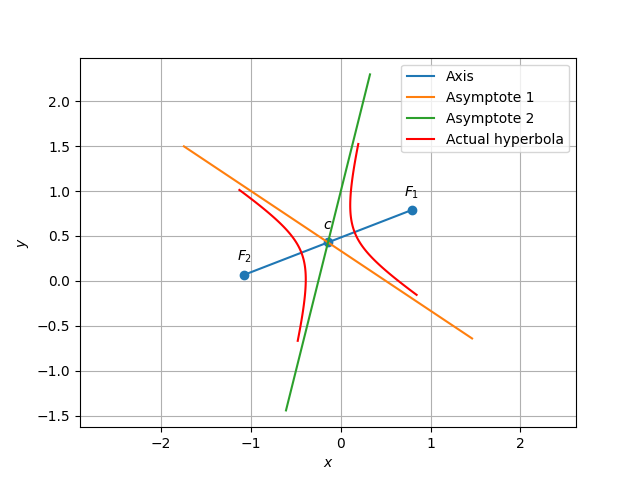
\includegraphics[width=\columnwidth]{./figs/asymp/hyper_asymp.png}
    \caption{Hyperbola with assymptotes and its conjugate}
    \label{eq:solutions/40/7/Fig :1}
\end{figure}
\end{enumerate}

%\section{Example: Pair of Straight Lines}
%\renewcommand{\theequation}{\theenumi}
\begin{enumerate}[label=\thesection.\arabic*.,ref=\thesection.\theenumi]
\numberwithin{equation}{enumi}

%\item Let the pair of straight lines be given by 
%\begin{align}
%\label{eq:quad_pair_lines}
%\vec{n}_1^T \vec{x} = c_1
%\\
%\vec{n}_2^T \vec{x} = c_2
%\end{align}
%Equating their product with \eqref{eq:conic_quad_form},
%\begin{multline}
%\brak{\vec{n}_1^T \vec{x} - c_1}
%\brak{\vec{n}_2^T \vec{x} - c_2} 
%\\
%=
%\vec{x}^T\vec{V}\vec{x}+2\vec{u}^T\vec{x}+f=0
%%\label{eq:quad_pair_lines}
%\end{multline}
%\begin{align}
%\implies 
%\vec{n}_1 *\vec{n}_2  &= \myvec{a \\ 2b \\c}
%\label{eq:quad_pair_conv}
%\\
%c_2\vec{n}_1 + c_1 \vec{n}_2 &= -2\vec{u}
%\label{eq:quad_pair_ci}
%\\
%c_1 c_2 &= f
%\label{eq:quad_pair_f}
%\end{align}
%%
%where $*$ represents convolution.
%\item The slopes of the lines are given by the roots of the polynomial
%\begin{align}
%\label{eq:quad_pair_slopes}
%cm^2 + 2bm + a = 0
%\\
%\implies m_i = \frac{-b \pm \sqrt{-\abs{V}}}{c}
%\end{align}
%and 
%\begin{align}
%\vec{n}_i = k_i\myvec{-m_i\\1}, \quad i = 1,2.
%\end{align}
%\item From \eqref{eq:quad_pair_ci},
%\begin{align}
%\label{eq:quad_pair_ci_mat}
%\myvec{\vec{n}_1 & \vec{n}_2}\myvec{c_2\\c_1} = -2\vec{u}
%\end{align}
%$c_1,c_2$ can be obtained such that they satisfy \eqref{eq:quad_pair_f}.

\item 
Given,
\begin{align}
    12x^2+7xy-10y^2+13x+45y-35&=0 
\label{eq:pair_given}
\end{align}

it is easy to verify that
\begin{align}
\mydet{
12 &\frac{7}{2}& \frac{13}{2}
\\
\frac{7}{2} & -10 & \frac{45}{2}
\\ 
\frac{13}{2} & \frac{45}{2} & -35
} = 0
\end{align}
%
Hence, \eqref{eq:pair_given} represents a pair of straight lines.

\item  \eqref{eq:pair_given} can be expressed as \eqref{eq:conic_quad_form} with
\begin{align}
    \vec{V}=\vec{V}^T&=\myvec{12 & \frac{7}{2}\\\frac{7}{2} &-10}\label{eq:pair_v}\\
    \vec{u}&=\myvec{\frac{13}{2} \\ \frac{45}{2}}\label{eq:pair_u}\\
    f&=-35\label{eq:pair_fv}
\end{align}
From \eqref{eq:pair_given} and \eqref{eq:quad_pair_slopes},
\begin{align}
\label{eq:quad_pair_slopes_ex}
\implies m_i &= \frac{-7 \pm \sqrt{49+480}}{-20}
\\
\implies m_1 &=  \frac{3}{2}, m_2 = -\frac{4}{5}
\end{align}
Thus,
\begin{align}
\vec{m}_1 = \myvec{2\\3},
\vec{m}_2 = \myvec{5\\-4}
\\
\implies
\vec{n}_1 = \myvec{3\\-2},
\vec{n}_2 = \myvec{4\\5}
\label{eq:quad_pair_norm_vec}
\end{align}
\item  Using the Toeplitz matrix,
\begin{align}
\vec{n}_1*\vec{n}_2 = 
\myvec{3 & 0
\\
-2 & 3
\\
0 & -2
}
\myvec{4\\5}
= \myvec{12 \\ 7 \\ -10}
\end{align}
%
which matches the corresponding coefficients in \eqref{eq:pair_given}

 Substituting from \eqref{eq:quad_pair_norm_vec}
in 
\eqref{eq:quad_pair_ci_mat}, 
the augmented matrix is
\begin{align}
\myvec{
3 & 4 & -13
\\
-2 & 5 & -45
}
\xleftrightarrow[R_1 \leftarrow \frac{R_1 - 4R_2}{3}]{R_2 \leftarrow \frac{2R_1 + 3R_2}{23}}
\myvec{
1 & 0 & 5
\\
0 & 1 & -7
}
\\
\implies c_1 = -7, c_2 = 5
\end{align}

Fig.     \ref{fig:pair} plots the lines in \eqref{eq:pair_given}
%
\begin{figure}[h]
    \centering
    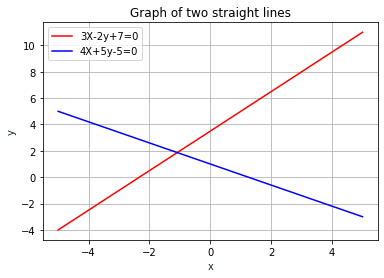
\includegraphics[width=\columnwidth]{./figs/pair/pair_ang.png}
    \caption{Pair of straight lines}
    \label{fig:pair}
\end{figure}

\item  From \eqref{eq:quad_pair_norm_vec}
the angle between the two straight lines is given by 
\begin{align}
    \theta&=\cos^{-1}\brak{\frac{\vec{n_1}^T\vec{n_2}}{\norm{\vec{n_1}}\norm{\vec{n_2}}}}
%\label{eq:pair_t}
\label{eq:pair_theta}
\\
    \vec{n_1}^T\vec{n_2}&=\myvec{3 & -2}\myvec{4\\5}=2\label{eq:pair_tr}\\
    \norm{\vec{n_1}}&=\sqrt{3^2+(-2)^2}=\sqrt{13}\label{eq:pair_norm1}\\
    \norm{\vec{n_2}}&=\sqrt{4^2+5^2}=\sqrt{41}\label{eq:pair_norm2}
\end{align}
Substituting equations \eqref{eq:pair_tr}, \eqref{eq:pair_norm1} ,\eqref{eq:pair_norm2} in equation \eqref{eq:pair_theta}, we get 
\begin{align}
        \theta&=\cos^{-1}\biggl(\frac{2}{\sqrt{13}\sqrt{41}}\biggr)\\
        \theta&=85\degree
\end{align}


\end{enumerate}


%\section{Convolution}
%\renewcommand{\theequation}{\theenumi}
\begin{enumerate}[label=\thesection.\arabic*.,ref=\thesection.\theenumi]
\numberwithin{equation}{enumi}

%\item Let the pair of straight lines be given by 
%\begin{align}
%\label{eq:quad_pair_lines}
%\vec{n}_1^T \vec{x} = c_1
%\\
%\vec{n}_2^T \vec{x} = c_2
%\end{align}
%Equating their product with \eqref{eq:conic_quad_form},
%\begin{multline}
%\brak{\vec{n}_1^T \vec{x} - c_1}
%\brak{\vec{n}_2^T \vec{x} - c_2} 
%\\
%=
%\vec{x}^T\vec{V}\vec{x}+2\vec{u}^T\vec{x}+f=0
%%\label{eq:quad_pair_lines}
%\end{multline}
%\begin{align}
%\implies 
%\vec{n}_1 *\vec{n}_2  &= \myvec{a \\ 2b \\c}
%\label{eq:quad_pair_conv}
%\\
%c_2\vec{n}_1 + c_1 \vec{n}_2 &= -2\vec{u}
%\label{eq:quad_pair_ci}
%\\
%c_1 c_2 &= f
%\label{eq:quad_pair_f}
%\end{align}
%%
%where $*$ represents convolution.
%\item The slopes of the lines are given by the roots of the polynomial
%\begin{align}
%\label{eq:quad_pair_slopes}
%cm^2 + 2bm + a = 0
%\\
%\implies m_i = \frac{-b \pm \sqrt{-\abs{V}}}{c}
%\end{align}
%and 
%\begin{align}
%\vec{n}_i = k_i\myvec{-m_i\\1}, \quad i = 1,2.
%\end{align}
%\item From \eqref{eq:quad_pair_ci},
%\begin{align}
%\label{eq:quad_pair_ci_mat}
%\myvec{\vec{n}_1 & \vec{n}_2}\myvec{c_2\\c_1} = -2\vec{u}
%\end{align}
%$c_1,c_2$ can be obtained such that they satisfy \eqref{eq:quad_pair_f}.

\item 
Given,
\begin{align}
    12x^2+7xy-10y^2+13x+45y-35&=0 
\label{eq:pair_given}
\end{align}

it is easy to verify that
\begin{align}
\mydet{
12 &\frac{7}{2}& \frac{13}{2}
\\
\frac{7}{2} & -10 & \frac{45}{2}
\\ 
\frac{13}{2} & \frac{45}{2} & -35
} = 0
\end{align}
%
Hence, \eqref{eq:pair_given} represents a pair of straight lines.

\item  \eqref{eq:pair_given} can be expressed as \eqref{eq:conic_quad_form} with
\begin{align}
    \vec{V}=\vec{V}^T&=\myvec{12 & \frac{7}{2}\\\frac{7}{2} &-10}\label{eq:pair_v}\\
    \vec{u}&=\myvec{\frac{13}{2} \\ \frac{45}{2}}\label{eq:pair_u}\\
    f&=-35\label{eq:pair_fv}
\end{align}
From \eqref{eq:pair_given} and \eqref{eq:quad_pair_slopes},
\begin{align}
\label{eq:quad_pair_slopes_ex}
\implies m_i &= \frac{-7 \pm \sqrt{49+480}}{-20}
\\
\implies m_1 &=  \frac{3}{2}, m_2 = -\frac{4}{5}
\end{align}
Thus,
\begin{align}
\vec{m}_1 = \myvec{2\\3},
\vec{m}_2 = \myvec{5\\-4}
\\
\implies
\vec{n}_1 = \myvec{3\\-2},
\vec{n}_2 = \myvec{4\\5}
\label{eq:quad_pair_norm_vec}
\end{align}
\item  Using the Toeplitz matrix,
\begin{align}
\vec{n}_1*\vec{n}_2 = 
\myvec{3 & 0
\\
-2 & 3
\\
0 & -2
}
\myvec{4\\5}
= \myvec{12 \\ 7 \\ -10}
\end{align}
%
which matches the corresponding coefficients in \eqref{eq:pair_given}

 Substituting from \eqref{eq:quad_pair_norm_vec}
in 
\eqref{eq:quad_pair_ci_mat}, 
the augmented matrix is
\begin{align}
\myvec{
3 & 4 & -13
\\
-2 & 5 & -45
}
\xleftrightarrow[R_1 \leftarrow \frac{R_1 - 4R_2}{3}]{R_2 \leftarrow \frac{2R_1 + 3R_2}{23}}
\myvec{
1 & 0 & 5
\\
0 & 1 & -7
}
\\
\implies c_1 = -7, c_2 = 5
\end{align}

Fig.     \ref{fig:pair} plots the lines in \eqref{eq:pair_given}
%
\begin{figure}[h]
    \centering
    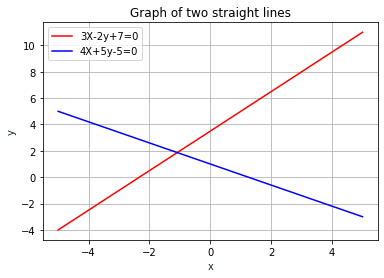
\includegraphics[width=\columnwidth]{./figs/pair/pair_ang.png}
    \caption{Pair of straight lines}
    \label{fig:pair}
\end{figure}

\item  From \eqref{eq:quad_pair_norm_vec}
the angle between the two straight lines is given by 
\begin{align}
    \theta&=\cos^{-1}\brak{\frac{\vec{n_1}^T\vec{n_2}}{\norm{\vec{n_1}}\norm{\vec{n_2}}}}
%\label{eq:pair_t}
\label{eq:pair_theta}
\\
    \vec{n_1}^T\vec{n_2}&=\myvec{3 & -2}\myvec{4\\5}=2\label{eq:pair_tr}\\
    \norm{\vec{n_1}}&=\sqrt{3^2+(-2)^2}=\sqrt{13}\label{eq:pair_norm1}\\
    \norm{\vec{n_2}}&=\sqrt{4^2+5^2}=\sqrt{41}\label{eq:pair_norm2}
\end{align}
Substituting equations \eqref{eq:pair_tr}, \eqref{eq:pair_norm1} ,\eqref{eq:pair_norm2} in equation \eqref{eq:pair_theta}, we get 
\begin{align}
        \theta&=\cos^{-1}\biggl(\frac{2}{\sqrt{13}\sqrt{41}}\biggr)\\
        \theta&=85\degree
\end{align}


\end{enumerate}


\subsection{Circle}
\iffalse
\documentclass[12pt]{article}
\usepackage{graphicx}
%\documentclass[journal,12pt,twocolumn]{IEEEtran}
\usepackage[none]{hyphenat}
\usepackage{graphicx}
\usepackage{listings}
\usepackage[english]{babel}
\usepackage{graphicx}
\usepackage{caption} 
\usepackage{hyperref}
\usepackage{booktabs}
\usepackage{commath}
\usepackage{gensymb}
\usepackage{array}
\usepackage{amsmath}   % for having text in math mode
\usepackage{listings}
\lstset{
  frame=single,
  breaklines=true
}
  
%Following 2 lines were added to remove the blank page at the beginning
\usepackage{atbegshi}% http://ctan.org/pkg/atbegshi
\AtBeginDocument{\AtBeginShipoutNext{\AtBeginShipoutDiscard}}
%


%New macro definitions
\newcommand{\mydet}[1]{\ensuremath{\begin{vmatrix}#1\end{vmatrix}}}
\providecommand{\brak}[1]{\ensuremath{\left(#1\right)}}
\providecommand{\norm}[1]{\left\lVert#1\right\rVert}
\newcommand{\solution}{\noindent \textbf{Solution: }}
\newcommand{\myvec}[1]{\ensuremath{\begin{pmatrix}#1\end{pmatrix}}}
\let\vec\mathbf
\begin{document}
\begin{center}
\title{\textbf{Circles}}
\date{\vspace{-5ex}} %Not to print date automatically
\maketitle
\end{center}
\setcounter{page}{1}
\section{11$^{th}$ Maths - Exercise 11.1.9}

\begin{enumerate}
\item Find the centre and radius of the given circle $2x^2+2y^2-x=0$
\section{Solution}
\fi
The given equation can be expressed as 
\begin{align}
	x^2+y^2-\frac{x}{2}&=0
	\\
\implies 	\norm{\vec{x}}^2+2\myvec{\frac{-1}{4} & 0}\vec{x}&=0
\end{align}	
The centre of circle is then given by 
\begin{align}
	\vec{u} = -\vec{c} 
=\myvec{\frac{1}{4}\\0}
\end{align}
and the radius of circle is obtained as
\begin{align}
	r=\sqrt{\norm{\vec{u}}^2 -f}
=\frac{1}{4}
\end{align}
See Fig. 
  \ref{fig:chapters/11/11/1/9/Figure}.
\begin{figure}[h]
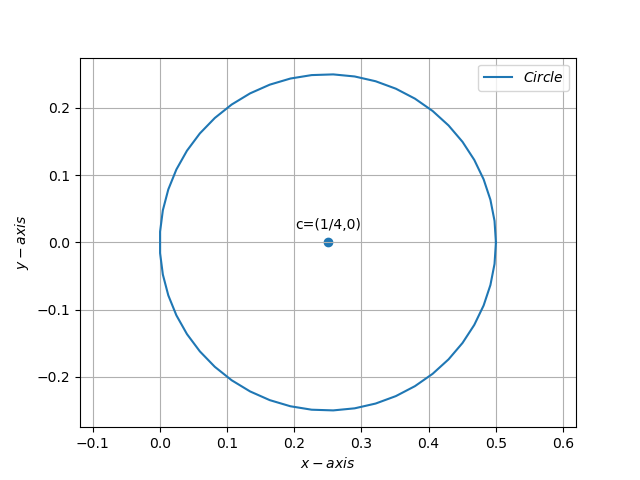
\includegraphics[width=\columnwidth]{chapters/11/11/1/9/figs/fig.png}
\caption{}
  \label{fig:chapters/11/11/1/9/Figure}
\end{figure}

\subsection{Ellipse}
\iffalse
\documentclass[12pt]{article}
\usepackage{graphicx}
\usepackage[none]{hyphenat}
\usepackage{graphicx}
\usepackage{listings}
\usepackage[english]{babel}
\usepackage{graphicx}
\usepackage{caption} 
\usepackage{booktabs}
\usepackage{array}
\usepackage{amssymb} % for \because
\usepackage{amsmath}   % for having text in math mode
\usepackage{extarrows} % for Row operations arrows
\usepackage{listings}
\lstset{
  frame=single,
  breaklines=true
}
\usepackage{hyperref}
  
%Following 2 lines were added to remove the blank page at the beginning
\usepackage{atbegshi}% http://ctan.org/pkg/atbegshi
\AtBeginDocument{\AtBeginShipoutNext{\AtBeginShipoutDiscard}}


%New macro definitions
\newcommand{\mydet}[1]{\ensuremath{\begin{vmatrix}#1\end{vmatrix}}}
\providecommand{\brak}[1]{\ensuremath{\left(#1\right)}}
\providecommand{\norm}[1]{\left\lVert#1\right\rVert}
\providecommand{\abs}[1]{\left\vert#1\right\vert}
\newcommand{\solution}{\noindent \textbf{Solution: }}
\newcommand{\myvec}[1]{\ensuremath{\begin{pmatrix}#1\end{pmatrix}}}
\let\vec\mathbf


\begin{document}

\begin{center}
\title{\textbf{Conic Sections - Ellipse}}
\date{\vspace{-5ex}} %Not to print date automatically
\maketitle
\end{center}
\setcounter{page}{1}

\section{11$^{th}$ Maths - Chapter 11}
This is Problem-7 from Exercise 11.5
\begin{enumerate}

\solution 
\fi
The conic section for the given problem is an ellipse. Let $\vec{O}\myvec{0 \\ 0}$ be the centre of the Ellipse. Then, the focii are given by 
\begin{align}
    \label{eq:chapters/11/11/5/7/ellipseEq1}
	\vec{F_1} = \myvec{ 4 \\ 0} \\
	\vec{F_2} = \myvec{ -4 \\ 0} 
\end{align}
The sum of the distances from two focii to the point on the locus of the ellipse is equal to $10m$. Let $\vec{P}\myvec{p \\ 0 }$ and $\vec{Q}\myvec{-q \\ 0}$ be the vertices of the ellipse. Then
\begin{align}
	\norm{\vec{P}-\vec{F_1}} + \norm{\vec{P}-\vec{F_2}} = 10 \\
         \brak{p-4} + \brak{p+4} = 10 \\
	 2p = 10 \\
	 p = 5  \\
	 \therefore \vec{P} = \myvec{5 \\ 0}
\end{align}
Similarly
\begin{align}
	\norm{\vec{Q}-\vec{F_1}} + \norm{\vec{Q}-\vec{F_2}} = 10 \\
         \brak{q-4} + \brak{q+4} = 10 \\
	 2q = 10 \\
	 q = 5 \\
	 \therefore \vec{Q} = \myvec{-5 \\ 0}
\end{align}
We know that the Vertex of a standard ellipse is given by
\begin{align}
	\vec{P} &=  \myvec{\sqrt{\abs{\frac{f_0}{\lambda_1}}} \\ 0} \\
	\myvec{5 \\ 0} &=  \myvec{\sqrt{\abs{\frac{f_0}{\lambda_1}}} \\ 0} \\
	\frac{f_0}{\lambda_1} &= 25 \\
	\label{eq:chapters/11/11/5/7/eqV}
	f_0 &= 25\lambda_1 
\end{align}
We know that the Focii for standard Ellipse are given as
\begin{align}
	\label{eq:chapters/11/11/5/7/eqV1}
	\vec{F} &= \pm e\sqrt{\frac{\abs{f_0}}{\lambda_2\brak{1-e^2}}}\vec{e}_1
\end{align}
Substituting values of $\vec{F_1}$ from \eqref{eq:chapters/11/11/5/7/ellipseEq1} and $f_0$ from \eqref{eq:chapters/11/11/5/7/eqV}
\begin{align}
	   \label{eq:chapters/11/11/5/7/eqV2}
	   \eqref{eq:chapters/11/11/5/7/eqV1} \implies \myvec{4 \\0}  &=e\sqrt{\frac{25\lambda_1}{\lambda_2\brak{1-e^2}}}\vec{e}_1
\end{align}
We know that 
\begin{align}
	1-e^2 = \frac{\lambda_1}{\lambda_2} \\
	\eqref{eq:chapters/11/11/5/7/eqV2} \implies  4 &= 5e \\
        e &= \frac{4}{5} \\
	\therefore \frac{\lambda_1}{\lambda_2} &= 1 - \brak{\frac{4}{5}}^2 \\
	&= \frac{9}{25} \\
	\vec{n} &= \sqrt{\frac{\lambda_2}{f_0}}\vec{e}_1\\
	 &= \sqrt{\frac{\lambda_2}{25\lambda_1}}\vec{e}_1\\
	 &= \frac{1}{5} \times \frac{5}{3}\vec{e}_1\\
	 &= \frac{1}{3}\vec{e}_1 \\
	 c &= \frac{1}{e\sqrt{1-e^2}} = \frac{25}{12}
\end{align}
For the standard ellipse, $f$ is given as 
\begin{align}
	\label{eq:chapters/11/11/5/7/eqV3}
	f &= \norm{\vec{n}}^2 \norm{\vec{F}}^2 - c^2 e^2 \\
	&= \brak{\frac{1}{3}}^216 - \frac{25}{9} \\
	&= -1 \\
	f_0 &= -f = 1 \\
	\lambda_1 &= \frac{f_0}{25} = \frac{1}{25}\\
	\lambda_2 &= \frac{25\lambda_1}{9} = \frac{1}{9} \\
	\therefore \vec{V} &= \myvec{\lambda_1 & 0 \\ 0 & \lambda_2} = \myvec{\frac{1}{25} & 0 \\ 0 & \frac{1}{9}}
\end{align}
For a standard ellipse, $\vec{u}=0$. 

The generic equation of conic section is given as
\begin{align}
	\label{eq:chapters/11/11/5/7/ellipseEq2}
	g\brak{\vec{x}} &= \vec{x}^T\vec{V}\vec{x} + 2\vec{u}^T\vec{x} + f = 0 \\ 
	&= \vec{x}^T\myvec{\frac{1}{25} & 0 \\ 0 & \frac{1}{9}}\vec{x}- 1  = 0 
\end{align}
The relevant diagram is shown in Figure \ref{fig:chapters/11/11/5/7/Fig1}
\begin{figure}[!h]
	\begin{center}
		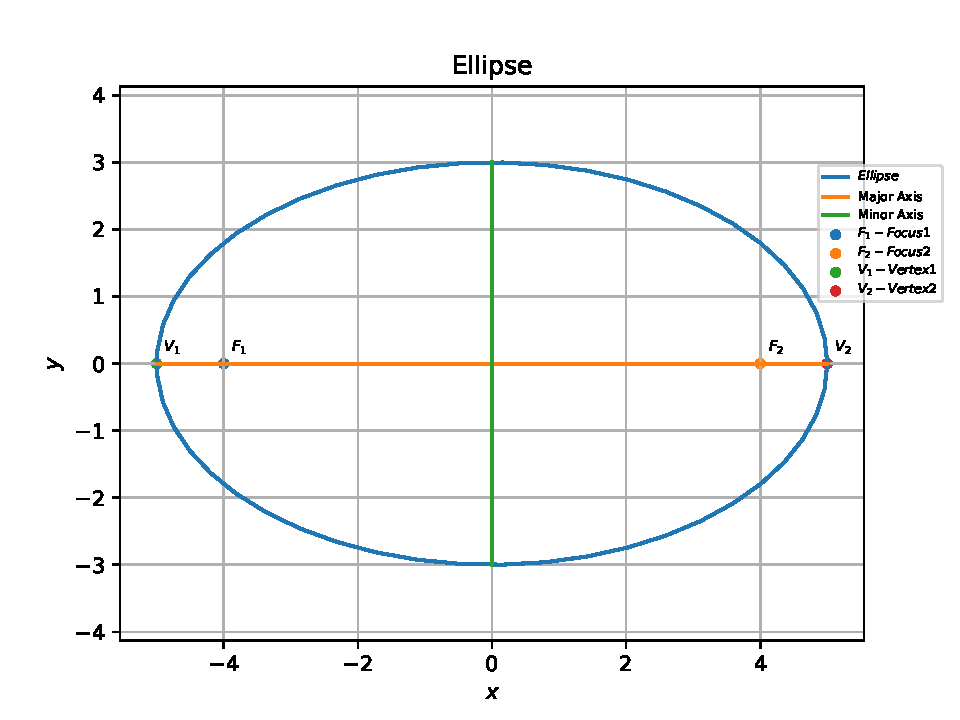
\includegraphics[width=\columnwidth]{chapters/11/11/5/7/figs/problem7.pdf}
	\end{center}
\caption{}
\label{fig:chapters/11/11/5/7/Fig1}
\end{figure}

\subsection{Hyperbola}
\renewcommand{\theequation}{\theenumi}
\begin{enumerate}[label=\thesubsection.\arabic*.,ref=\thesubsection.\theenumi]
\numberwithin{equation}{enumi}
\item 
Find the equation of all lines having slope 2 and being tangent to the curve 
%\cite{twelve_one}
\begin{align}
\label{eq:hyperbola}
y + \frac{2}{x-3} = 0
\end{align}
\solution 
\eqref{eq:hyperbola} can be expressed as
\begin{align}
\label{eq:conic_nofrac}
xy -3y + 2 = 0
\end{align}
which is of the same form as \eqref{eq:conic_quad_form} with 
\begin{align}
\label{eq:hyper_quad_form_param}
\vec{V} = \frac{1}{2}\myvec{0 & 1\\ 1 & 0}, \vec{u} = -\frac{3}{2}\myvec{0 \\1}, f = 2
\end{align}
Using the approach in Example \ref{ex:ellipse_tangent},
\begin{align}
\vec{D} = \myvec{\frac{1}{2} & 0 \\ 0 & -\frac{1}{2}}, \vec{P} = \frac{1}{\sqrt{2}}\myvec{1 & -1\\1 & 1}
\end{align}
\begin{align}
\because \vec{u}^T\vec{V}^{-1}\vec{u}-f = -2 < 0,
\end{align} 
the major and minor axis are swapped and from Table \ref{table:conics}
the hyperbola parameters are given by 
\begin{align}
\vec{c}= 3\myvec{1\\0},
\sqrt{\frac{\vec{u}^T\vec{V}^{-1}\vec{u}-f}{\lambda_2}} = 2,
\\
\sqrt{\frac{f-\vec{u}^T\vec{V}^{-1}\vec{u}}{\lambda_1}} = 2
\end{align}
with the standard hyperbola equation becoming
\begin{align}
\frac{y_2^2}{4}-\frac{y_1^2}{4} = 1,
\label{eq:std_hyper}
\end{align}
%
Fig. \ref{fig:hyper_tangent}	shows  the actual hyperbola in \eqref{eq:hyperbola}  obtained from  
\eqref{eq:std_hyper}  using \eqref{eq:conic_affine}.  
The direction and normal vectors of the tangent with slope 2 are given by \eqref{eq:dir_vec_slope} and \eqref{eq:line_dir_norm} as
\begin{align}
\vec{m} = \myvec{1\\2}, \vec{n} = \myvec{2\\-1}
\end{align}
%
From \eqref{eq:conic_tangent_qk} and \eqref{eq:circle_tangent_prob_uf}, using \eqref{eq:hyper_quad_form_param},
\begin{align}
\kappa = \frac{1}{2}, \vec{q}_1 = \myvec{2\\2}, \vec{q}_2 = \myvec{4\\-2}.
\end{align}
%
The desired tangents are
\begin{align}
\myvec{2 & -1}\cbrak{\vec{x}-\myvec{2\\2}} &= 0 \implies \myvec{2 & -1} \vec{x} = 2
\\
\myvec{2 & -1}\cbrak{\vec{x}-\myvec{4\\-2}} &= 0 \implies \myvec{2 & -1} \vec{x} = 10
\end{align}
All the above results are verified in Fig. \ref{fig:hyper_tangent}.  As we can see, the hyperbola in \eqref{eq:hyperbola} is obtained by rotating the standard hyperbola by $\vec{P}$	and then translating it by $\vec{c}$.

\begin{figure}[!ht]
\centering
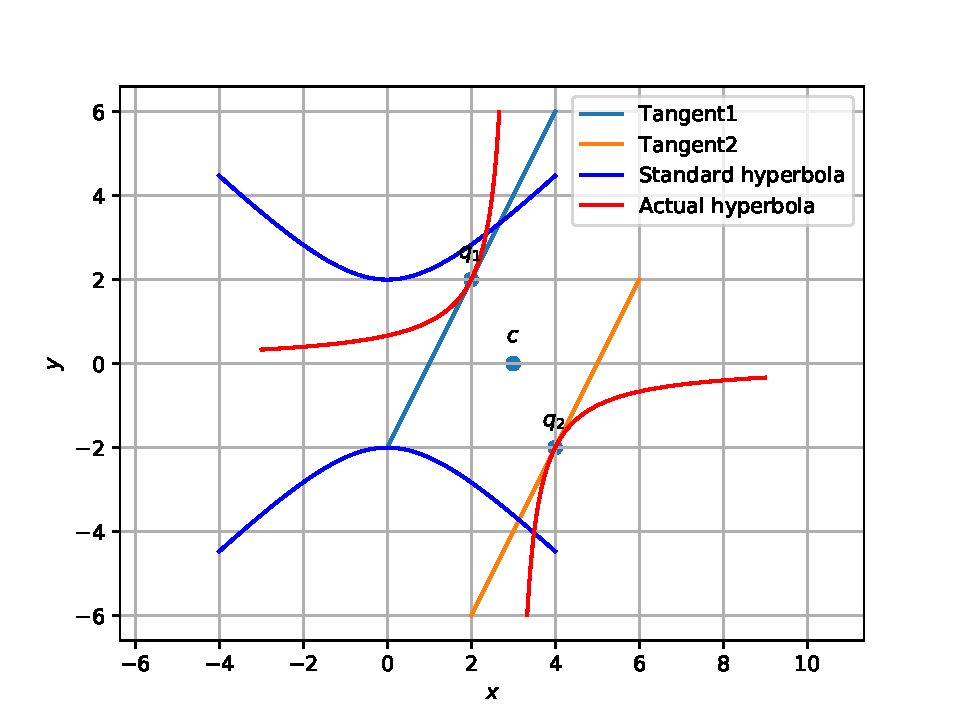
\includegraphics[width=\columnwidth]{./figs/hyper/hyper_tangent.eps}
\caption{Standard and actual hyperbola.}
\label{fig:hyper_tangent}	
\end{figure}
\item Find the asymptotes of the hyperbola given below and also the equations to their conjugate hyperbolas.
\begin{align}
\label{eq:hyper_asymp}
8x^2+10xy-3y^2-2x+4y-2=0
\end{align}
\begin{enumerate}
\item  \eqref{eq:hyper_asymp} can be expressed as \eqref{eq:conic_quad_form} with 
\begin{align}
    \vec{V}=\vec{V}^T&=\myvec{8 & 5 \\ 5 &-3}\label{eq:solutions/40/7/eqv}\\
    \vec{u}&=\myvec{-1 \\2 }\label{eq:solutions/40/7/equ}\\
    f&=-2\label{eq:solutions/40/7/eqfv}
\end{align}   
Expanding the Determinant of $\vec{V}$,
\begin{align}
    \Delta_{V} &= \mydet
%\begin{array}{|cc|}
{
8 &5
\\
5 & -3
}
= -49 < 0
%\end{array}<0
\label{eq:solutions/40/7/eq:hyp}
\end{align}
Hence from \eqref{eq:conic_hyper_cond} and \eqref{eq:solutions/40/7/eq:hyp}, \eqref{eq:hyper_asymp}
%\eqref{eq:solutions/40/7/eq:hyp} 
represents a hyperbola.
The characteristic equation of $\vec{V}$ is obtained by evaluating the determinant 
\begin{align}
%       \begin{array}{|c|}
\mydet{V-\lambda\vec{I}} = 0
\\
%\end{array}&=0\\
%   \begin{array}{|cc|}
\mydet{
8-\lambda & 5 \\ 5 & -3-\lambda
} = 0
\\
%\end{array}&=0\\
    \brak{8-\lambda}\brak{-3-\lambda}-25=0\\
\implies \lambda^2 -5\lambda -49 = 0
\label{eq:asymptotes_char}
\\
    \lambda_{1}= \frac{5+\sqrt{221}}{2}\label{eq:solutions/40/7/eq:matrix_l1}\\
    \lambda_{2}= \frac{5-\sqrt{221}}{2}\label{eq:solutions/40/7/eq:matrix_l2}
\end{align}
The eigenvector $\vec{p}$ is defined as 
\begin{align}
    \vec{V}\vec{p}&=\lambda\vec{p}\\
    \implies (\vec{V}-\lambda\vec{I})\vec{p}&=0\label{eq:solutions/40/7/eq:7/eqev}
\end{align}
For $\lambda_1=\frac{5+\sqrt{221}}{2}$ ,
\begin{align}
    (\vec{V}-\lambda_1\vec{I})=\myvec{\frac{11-\sqrt{221}}{2} & 5 \\5 & \frac{-11-\sqrt{221}}{2}}
\end{align}
By row reduction, 
\begin{align}
    &\myvec{\frac{11-\sqrt{221}}{2} & 5 \\5 & \frac{-11-\sqrt{221}}{2}}\\
    %&\xleftrightarrow{\frac{R_1}{\frac{\sqrt{533}+2}{2}}}\\
%    &\xleftrightarrow{R_1\leftarrow R_2}
%    \myvec{\frac{-11-\sqrt{221}}{2} & 5 \\ \frac{11-\sqrt{221}}{2} & 5}\\
 &\xleftrightarrow{R_2\leftarrow R_2+\frac{11+\sqrt{221}}{10}R_{1}}
    \myvec{5 & \frac{-11-\sqrt{221}}{2} \\ 0& 0}%\\
%     &\xleftrightarrow{R_1\leftarrow R_1/5}
%    \myvec{1 & \frac{-11-\sqrt{221}}{10} \\ 0& 0}
    \label{eq:solutions/40/7/eq:7/eqs1}
\end{align}
Substituting \eqref{eq:solutions/40/7/eq:7/eqs1} in \eqref{eq:solutions/40/7/eq:7/eqev} we get
\begin{align}
        & \myvec{5 & \frac{-11-\sqrt{221}}{2} }\vec{p}_1=\vec{0}
\\
\implies \vec{p}_1 &= k \myvec{ \frac{11+\sqrt{221}}{2} \\ 5}
\label{eq:solutions/40/7/eq:7/eqei1}
\end{align}
For $\lambda_2=\frac{5-\sqrt{221}}{2}$ ,
\begin{align}
    (\vec{V}-\lambda_2\vec{I})=\myvec{\frac{11+\sqrt{221}}{2} & 5 \\5 & \frac{-11+\sqrt{221}}{2}}
\end{align}
By row reduction , 
\begin{align}
     \myvec{\frac{11+\sqrt{221}}{2} & 5 \\5 & \frac{-11+\sqrt{221}}{2}}
\\
    \xleftrightarrow{R_2\leftarrow R_2+ \frac{11-\sqrt{221}}{10}R_1}
     \myvec{\frac{11+\sqrt{221}}{2} &5\\ 0& 0}
    \label{eq:solutions/40/7/eq:es71/eqs2}
\end{align} 
Substiuting \eqref{eq:solutions/40/7/eq:es71/eqs2} in \eqref{eq:solutions/40/7/eq:7/eqev} we get 
\begin{align}
     \myvec{\frac{11+\sqrt{221}}{2} &5}\vec{p}_2=\vec{0}
\\
\implies \vec{p}_2 &= k \myvec{ -5 \\ \frac{11+\sqrt{221}}{2}}
\label{eq:solutions/40/7/eq:es71/eqei2}
\end{align}
Thus, we obtain 
\begin{align}
\vec{P} &= \myvec{\vec{p}_1 & \vec{p}_2}
= k \myvec{ \frac{11+\sqrt{221}}{2} & -5  \\ 5 & \frac{11+\sqrt{221}}{2}}
\end{align}
%
For
\begin{align}
\vec{P}^{\top}\vec{P} &= \vec{I},
k = \sqrt{\frac{221+11\sqrt{221}}{2}}
\end{align}
\begin{multline}
\implies \vec{P} = \sqrt{\frac{2}{221+11\sqrt{221}}}
\\
\times \myvec{ \frac{11+\sqrt{221}}{2} & -5  \\ 5 & \frac{11+\sqrt{221}}{2}}
\label{eq:solutions/40/7/eq:es71/eqP}
\end{multline}
and
\begin{align}
    \vec{V}&=\vec{P}\vec{D}\vec{P}^T\label{eq:solutions/40/7/eq:es71/eqsubs}
\end{align}
where 
\begin{align}
       \vec{D}&=\myvec{\frac{5+\sqrt{221}}{2} & 0\\0 & \frac{5-\sqrt{221}}{2}}\label{eq:solutions/40/7/eq:es71/eqDD}
\end{align}
Centre of the hyperbola is given by 
\begin{align}
    \vec{c}&=-\vec{V}^{-1}\vec{u}\\
    \implies\vec{c}&=-\myvec{\frac{3}{49}&\frac{5}{49}\\\frac{5}{49}&\frac{-8}{49}}\myvec{-1 \\ 2}\\
    \implies\vec{c}&=\myvec{\frac{-3}{49}&\frac{-5}{49}\\\frac{-5}{49}&\frac{8}{49}}\myvec{-1 \\ 2}\\
    \implies\vec{c}&=\myvec{\frac{-1}{7}\\\frac{3}{7}}
\end{align}
Since,
\begin{align}
    \vec{u}^T\vec{V}^{-1}\vec{u}-f = 1 > 0\label{eq:solutions/40/7/eq:es71/cond}
\end{align} 
there isn't a need to swap axes
In hyperbola,
\begin{align}
axes=
\begin{cases}
\sqrt{\frac{\vec{u}^T\vec{V}^{-1}\vec{u}-f}{\lambda_1}}\\ \sqrt{\frac{f-\vec{u}^T\vec{V}^{-1}\vec{u}}{\lambda_2}}
\end{cases}
\end{align}
From above equations we can say that,
\begin{align}
\sqrt{\frac{\vec{u}^T\vec{V}^{-1}\vec{u}-f}{\lambda_1}}=\sqrt{ \frac{2}{5+\sqrt{221}}}\\
\sqrt{\frac{f-\vec{u}^T\vec{V}^{-1}\vec{u}}{\lambda_2}}=\sqrt{ \frac{2}{5-\sqrt{221}}}
\end{align}
The equation of the hyperbola at the origin is then given by \eqref{eq:conic_simp_temp_nonparab} as
 %Now we have,
\begin{align}
    \vec{y}^T\vec{D}\vec{y}=\vec{u}^T\vec{V}^{-1}\vec{u}-f\label{eq:solutions/40/7/eq:es71/fi}
\\
   \implies\vec{y}^T\myvec{\frac{5+\sqrt{221}}{2} & 0 \\0 & \frac{5-\sqrt{221}}{2}}\vec{y}= 1
\end{align}
\item ({\em Asymptotes of hyperbola: })
The equation for the asymptotes of \eqref{eq:hyper_asymp} is given by \eqref{eq:asymp_quad_form} with 
\begin{align} 
K &=  \vec{u}^T\vec{V}^{-1}\vec{u}
\\
&=   \myvec{-1 & 2 }  \myvec{8 & 5 \\ 5 &-3}^{-1}\myvec{-1 \\2 }
 =-1
\label{eq:quad_form_asymp_condK}
\end{align}
%
From \eqref{eq:quad_form_pair_normvecs}, \eqref{eq:solutions/40/7/eq:matrix_l1} and \eqref{eq:solutions/40/7/eq:matrix_l2},
%
\begin{multline}
\vec{n}_1 =  \sqrt{\frac{2}{221+11\sqrt{221}}}
\\
\times \myvec{ \frac{11+\sqrt{221}}{2} & 5  \\ -5 & \frac{11+\sqrt{221}}{2}}
\\
\times \myvec{\sqrt{\frac{\sqrt{221}+5}{2}} \\  \sqrt{\frac{\sqrt{221}-5}{2}}}
%\label{eq:solutions/40/7/eq:es71/eqP}
\end{multline}
%
which can be expressed as
%
\begin{multline}
\vec{n}_1 = 
 \frac{1}{\sqrt{\brak{\lambda+3}^2+5^2}}
\\
\times \myvec{ \lambda_1+3 & 5  \\ -5 & \lambda_1+3}
\myvec{\sqrt{\lambda_1} \\  \frac{7}{\sqrt{\lambda_1}}}
%\label{eq:solutions/40/7/eq:es71/eqP}
\end{multline}
%
which is equivalent to
%
\begin{align}
\vec{n}_1 &= 
\myvec{ \lambda_1+3 & 5  \\ -5 & \lambda_1+3}\myvec{\lambda_1 \\  7}
\\
&= \myvec{ \lambda^2_1+3\lambda_1 +35  \\ 2\lambda_1 +21}
\\
&= \myvec{ 8\lambda_1 +84  \\ 2\lambda_1 +21}
%\label{eq:solutions/40/7/eq:es71/eqP}
\end{align}
using \eqref{eq:asymptotes_char}, which is equivalent to
\begin{align}
\vec{n}_1 &= \myvec{4 \\ 1}
\end{align}
%
Similarly, it can be shown that 
\begin{align}
\vec{n_2}&=\myvec{2\\3} \label{eq:solutions/40/7/eq:normal1}
\end{align}
%
%\item {Conjugate Hyperbola: }  The angle between the asymptotes is obtained from \eqref{eq:solutions/40/7/eq:matrix_l1} and \eqref{eq:solutions/40/7/eq:matrix_l2} as
%\begin{align}
%	\cos\theta=\brak{\frac{5}{\sqrt{221}}},
%	\sin\theta=\brak{\frac{14}{\sqrt{221}}}
%\end{align}
%%
%Consequently, the rotation matrix 
%\begin{align}
%\label{eq:asymp_conj_rot_mat}
%\vec{Q} = \frac{1}{\sqrt{221}}\myvec{
%5 & -14
%\\
%14 & 5
%} 
%\end{align}
%and the conjugate hyperbola is obtained from 
%\eqref{eq:hyper_asymp} and  \eqref{eq:conic_quad_form_conjugate}.
%as 
%
Fig.     \ref{eq:solutions/40/7/Fig :1} plots the hyperbola in \eqref{eq:hyper_asymp} along with the asymptotes obtained using \eqref{eq:quad_form_pair}.
 

\begin{figure}[!ht]
    \centering
    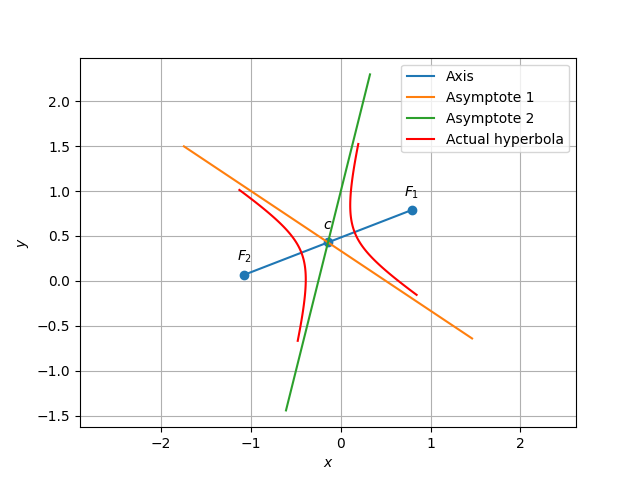
\includegraphics[width=\columnwidth]{./figs/asymp/hyper_asymp.png}
    \caption{Hyperbola with assymptotes and its conjugate}
    \label{eq:solutions/40/7/Fig :1}
\end{figure}
\end{enumerate}

\end{enumerate}

\subsection{Parabola}
\renewcommand{\theequation}{\theenumi}
\begin{enumerate}[label=\thesubsection.\arabic*.,ref=\thesubsection.\theenumi]
\numberwithin{equation}{enumi}
\item 
Find the point at which the tangent to the curve 
%\cite{twelve_one}
\begin{align}
y = \sqrt{4x-3}-1
\label{eq:parab}
\end{align}
has slope $\frac{2}{3}$.
\\
\solution \eqref{eq:parab} can be expressed as
\begin{align}
\brak{y+1}^2 &= 4x-3
\\
\text{or, } y^2  -4x + 2y+ 4 &= 0
\label{eq:parab_twovar}
\end{align}
which has the form \eqref{eq:conic_quad_form} with parameters
\begin{align}
\vec{V} = \myvec{0 & 0\\0 & 1}, \vec{u} = \myvec{-2\\1}, f = 4.
\label{eq:parab_twovar_params}
\end{align}
Thus, the given curve is a parabola.  $\because \vec{V}$ is diagonal and in standard form,
\begin{align}
\vec{P} = \vec{I} \implies \vec{p}_1 = \myvec{1\\0}
\label{eq:parab_ex1_eig}
\end{align}
From Table \ref{table:conics}, the 
focus is 4
and the vertex $\vec{c}$ is
\begin{align}
\myvec{ -4 & 1 \\ 0 & 0 \\ 0 & 1}\vec{c} &= \myvec{-4 \\ 0\\-1} 
\\
\implies 
\myvec{ -4 & 1 \\  0 & 1}\vec{c} &= \myvec{-4 \\ -1} 
\\
\text{or, } \vec{c} = \myvec{\frac{3}{4}\\-1}
\end{align}
The direction vector and normal vectors are
\begin{align}
\vec{m} = \myvec{1 \\ \frac{2}{3}} = \myvec{3\\2}, \vec{n} = \myvec{2\\-3}.
\label{eq:parab_twovar_mn}
\end{align}
Also, 
\begin{align}
\vec{V}\vec{p} &= \vec{0}
\\
\implies \vec{p} &= \myvec{1\\0}
\label{eq:parab_twovar_p}
\end{align}
From \eqref{eq:conic_tangent_qk_eigen}, \eqref{eq:parab_twovar_mn} and \eqref{eq:parab_twovar_p},
\begin{align}
\kappa = -1
\end{align}
which, upon substitution in \eqref{eq:conic_tangent_q_eigen} and simplification yields the matrix equation
\begin{align}
\myvec{-4 & 4\\0 & 0\\0&1}\vec{q} &= \myvec{-4\\0\\2}
\\
\implies \myvec{-4 & 4\\0&1}\vec{q} &= \myvec{-4\\2}
\\
\text{or, } \vec{q} &= \myvec{3\\2}
\end{align}
Fig. \ref{fig:parab_tangent}	verifies the above results.
%
\begin{figure}[!ht]
\centering
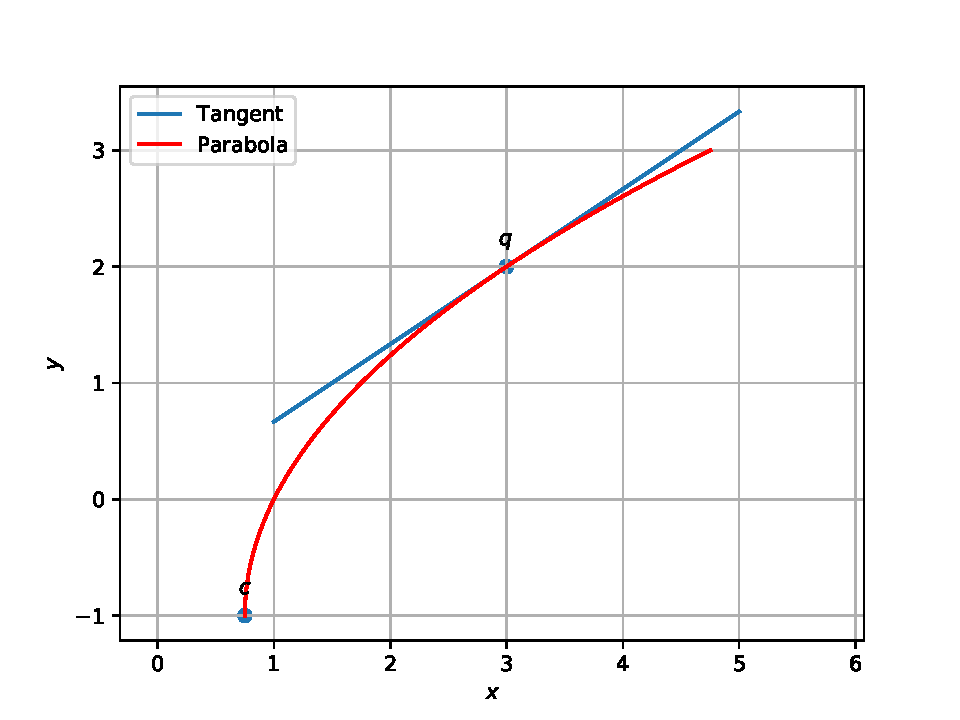
\includegraphics[width=\columnwidth]{./figs/parab/parab_tangent.eps}
\caption{Tangent to  parabola in \eqref{eq:parab}  with slope $\frac{2}{3}$. }
\label{fig:parab_tangent}	
\end{figure}

\item 
Find a point on the curve 
%\cite{twelve_one}
\begin{align}
y = \brak{x-2}^2
\label{eq:parab_secant}
\end{align}
at which the tangent is parallel to the chord joining the points (2, 0) and (4, 4).
\\
\solution \eqref{eq:parab_secant} can be expressed as
\begin{align}
x^2  -4x - y + 4 &= 0
\label{eq:parab_secant_twovar}
\end{align}
which has the form \eqref{eq:conic_quad_form} with parameters
\begin{align}
\vec{V} = \myvec{1 & 0\\0 & 0},  \vec{u} = -\myvec{2\\\frac{1}{2}}, f = 4.
\label{eq:parab_secant_twovar_params}
\end{align}
Using eigenvalue decomposition, 
\begin{align}
\vec{P} = \myvec{0 & 1\\1 & 0}, \vec{D} = \myvec{0 & 0\\0 & 1}
\end{align}
%
Hence, the eigenvector of $\vec{V}$ corresponding to the zero eigenvalue is
\begin{align}
\vec{p}_1 = \myvec{0\\1}.
\end{align}
Substituting the above parameters in the equation for the vertex of the parabola in Table \ref{table:conics},
\begin{align}
\myvec{-2 & -\frac{5}{2} \\ 1 & 0 \\ 0 & 0}\vec{c} &= \myvec{-4 \\ 2 \\ 0}
\\
\implies \myvec{-1 & -\frac{5}{2} \\ 1 & 0}\vec{c} &= \myvec{-4 \\ 2 }
\\
\text{or, } \vec{c} &= \myvec{2\\0}
\end{align}
The direction vector is
\begin{align}
\vec{m} = \myvec{4 \\ 4}-\myvec{2 \\ 0} = \myvec{1\\2}
\label{eq:parab_secant_twovar_m}
\end{align}
and normal vector is
\begin{align}
\vec{n} =  \myvec{2\\-1}
\label{eq:parab_secant_twovar_n}
\end{align}
From the equation for the point of contact for the  parabola  in Table \ref{table:conics},
%\eqref{eq:conic_tangent_qk_eigen}, \eqref{eq:parab_secant_twovar_params}
% and \eqref{eq:parab_secant_twovar_n} 
\begin{align}
\kappa = \frac{1}{2}
\end{align}
resulting in the matrix equation
\begin{align}
\myvec{-1 & -1\\1 & 0\\0&0}\vec{q} &= \myvec{-4\\3\\0}
\\
\implies \myvec{-1 & -1\\1 & 0}\vec{q} &= \myvec{-4\\3}
\\
\text{or, } \vec{q} &= \myvec{3\\1}
\end{align}
Fig. \ref{fig:parab_secant_tangent}	verifies the above results.  Note that $\vec{P}$ rotates the standard parabola by 90\degree.
%
\begin{figure}[!ht]
\centering
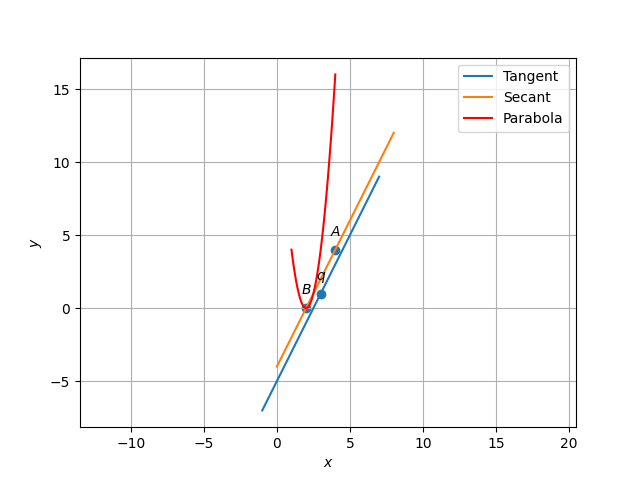
\includegraphics[width=\columnwidth]{./figs/parab/parab_tangent_secant.eps}
\caption{Tangent to  parabola in \eqref{eq:parab_secant}  is parallel to the line joining the points \myvec{2\\ 0} and \myvec{4\\ 4}. }
\label{fig:parab_secant_tangent}	
\end{figure}
%
\item What conic does the following equation represent. 
\begin{align}
9x^2-24xy+16y^2-18x-101y+19 = 0
\label{eq:conics/ex/solution/given}
\end{align}
Find the center.
%
\\
\solution
From \eqref{eq:conics/ex/solution/given} and \eqref{eq:conic_quad_form},
%
%\begin{align}
%\vec{x^T}\vec{V}\vec{x}+2\vec{u^T}\vec{x}+f=0\label{eq:conics/ex/solution/eqmain}
%\end{align}
%From the given second degree equation we get,
\begin{align}
\vec{V} &= \myvec{9&-12\\-12&16}\\ \label{eq:conics/ex/solution/given1}
\vec{u} &= \myvec{-9\\-\frac{101}{2}}\\ 
f &= 4 \label{eq:conics/ex/solution/given2}
\end{align}
\begin{enumerate}
\item Expanding the determinant of $\vec{V}$ we observe, 
\begin{align}
\mydet{9&-12\\-12&16} = 0 \label{eq:conics/ex/solution/eq2.1}
\end{align}
Also
\begin{align}
    \mydet{\vec{V} & \vec{u} \\ \vec{u}^T & f}=
    \mydet{9&-12 & -9 \\-12&16 & -\frac{101}{2} \\ -9 & -\frac{101}{2} & 4} \\
    \neq 0\label{eq:conics/ex/solution/eq2.2}
\end{align}
Hence from \eqref{eq:conics/ex/solution/eq2.1} and \eqref{eq:conics/ex/solution/eq2.2} we conclude that given equation is an parabola. The characteristic equation of $\vec{V}$ is given as follows,
\begin{align}
\mydet{\lambda\vec{I}-\vec{V}} = \mydet{\lambda-9&12\\12&\lambda-16} &= 0\\
\implies \lambda^2-25\lambda &= 0\label{eq:conics/ex/solution/eqchar}
\end{align}
Hence the characteristic equation of $\vec{V}$ is given by \eqref{eq:conics/ex/solution/eqchar}. The roots of \eqref{eq:conics/ex/solution/eqchar} i.e the eigenvalues are given by
\begin{align}
\lambda_1=0, \lambda_2=25\label{eq:conics/ex/solution/eqeigenvals}    
\end{align}
\item For $\lambda_1 = 0$, the eigen vector $\vec{p}$ is given by 
\begin{align}
\vec{V}\vec{p} = 0
%\\
%\brak{\lambda\vec{I}-\vec{V}}\vec{p}&=0 \label{eq:conics/ex/solution/eqev}
\end{align}
Row reducing $\vec{V}$ yields
\begin{align}
\implies
%\brak{\lambda_1\vec{I}-\vec{V}}&=
\myvec{-9&12\\12&-16}\xleftrightarrow[R_2=R_2+4R_1]{R_1=-\frac{R_1}{3}}\myvec{3&-4\\0&0}\\
\implies\vec{p}_1=\frac{1}{5}\myvec{-4\\-3} \label{eq:conics/ex/solution/eq2.3}
\end{align}
Similarly, 
\begin{align}
\vec{p}_2=\frac{1}{5}\myvec{-3\\4} 
%\label{eq:conics/ex/solution/eq2.3}
\end{align}
%
Thus, the eigenvector rotation matrix and the eigenvalue matrix are
%Substiuting equation \ref{eq:conics/ex/solution/eq2.3} in equation \ref{eq:conics/ex/solution/eqev} we get
%\begin{align}
%&\myvec{1&-\frac{4}{3}\\0&0}\myvec{v_1 \\ v_2}=\myvec{0 \\ 0}
%%\label{eq:conics/ex/solution/eqei1}
%\end{align}
%Where, $\vec{p}=\myvec{v_1\\v_2}$
%Let $v_2=t$
%\begin{align}
%    v_1&=\frac{4}{3}t
%\end{align}
%Eigen vector $\vec{p_1}$ is given by
%\begin{align}
%    \vec{p_1}&=\myvec{\frac{4}{3}t \\ t}
%\end{align}
%Let $t=-\frac{6}{10}$, we get
%\begin{align}
%        \vec{p_1}&=\myvec{-\frac{8}{10} \\-\frac{6}{10} }\label{eq:conics/ex/solution/eqp1}
%\end{align}
%Again, for $\lambda_2=25$,
%\begin{align}
%\brak{\lambda_2\vec{I}-\vec{V}}&=\myvec{16&12\\12&9}\xleftrightarrow[R_1=\frac{1}{16}R_1]{R_2=12R_1-R_2}\myvec{1&\frac{3}{4}\\0&0} \label{eq:conics/ex/solution/eq2.3.1}
%\end{align}
%Substiuting equation \ref{eq:conics/ex/solution/eq2.3.1} in equation \ref{eq:conics/ex/solution/eqev} we get
%\begin{align}
%&\myvec{1&\frac{3}{4}\\0&0}\myvec{v_1 \\ v_2}=\myvec{0 \\ 0}
%%\label{eq:conics/ex/solution/eqei1}
%\end{align}
%Where, $\vec{p}=\myvec{v_1\\v_2}$
%Let $v_2=t$
%\begin{align}
%    v_1&=-\frac{3}{4}t
%\end{align}
%Eigen vector $\vec{p_2}$ is given by
%\begin{align}
%    \vec{p_2}&=\myvec{-\frac{3}{4}t \\ t}
%\end{align}
%Let $t=-\frac{8}{10}$, we get
%\begin{align}
%        \vec{p_2}&=\myvec{\frac{6}{10} \\-\frac{8}{10} }
%%\label{eq:conics/ex/solution/eqp1}
%\end{align}
%The matrix $\vec{P}$,
\begin{align}
\vec{P}&=\myvec{\vec{p_1}&\vec{p_2}}=\frac{1}{5}\myvec{-4&-3\\ -3 &4} \\
\vec{D}&=\myvec{0&0\\0&25}
\end{align}
Table \ref{table:conics}, the focal length of the parabola is given by 
\begin{align}
\frac{\abs{2\vec{u}^T\vec{p_1}}}{\lambda_2}
    = \frac{75}{25}=3
\end{align}
%When $\mydet{\vec{V}}=0$,
%From 
%\eqref{eq:conics/ex/solution/eqmain} can be written as
and its equation is
\begin{align}
    \vec{y^T}\vec{D}\vec{y}&=-2\eta\myvec{1&0}\vec{y}\label{eq:conics/ex/solution/eq2.4}
\end{align}
where
\begin{align}
    \eta=\vec{u}^T\vec{p_1}=\frac{75}{2}
\end{align}
\begin{align}
    \myvec{\vec{u^T}+\eta\vec{p_1^T} \\ \vec{V}}\vec{c}=
    \myvec{-f \\ \eta\vec{p_1}-\vec{u}} 
\end{align}
using equations \eqref{eq:conics/ex/solution/given1},\eqref{eq:conics/ex/solution/given2} and \eqref{eq:conics/ex/solution/eq2.3}
\begin{align}
    \myvec{-39& -73 \\ 9 & -12 \\  -12 & 16 }\vec{c}=\myvec{-19 \\ -21\\ 28} \label{eq:conics/ex/solution/eqcen}
\end{align}
Forming the augmented matrix and row reducing it:
\begin{align}
\myvec{-39 & -73 & -19\\9 & -12 & -21 \\-12 & 16 &28 }\\
\xleftrightarrow[]{R_3\leftarrow R_3+(4/3)R_2} 
\myvec{-39 & -73 & -19\\9 & -12 & -21 \\0 & 0 &0 }\\
\xleftrightarrow[]{R_1\leftarrow R_1/(-39)} 
\myvec{1 & 73/39 & 19/39\\9 & -12 & -21 \\0 & 0 &0 }\\
\xleftrightarrow[]{R_2\leftarrow R_2-9R_1}
\myvec{1 & 73/39 & 19/39\\0 & -1125/39 & -990/39 \\0 & 0 &0}\\ 
\xleftrightarrow[]{R_2\leftarrow R_2 \times (-39/1125)}
\myvec{1 & 73/39 & 19/39\\0 & 1 & 22/25 \\0 & 0 &0}\\
\xleftrightarrow[]{R_1\leftarrow R_1 -(73/39)R_2}
\myvec{1 & 0 & -29/25\\0 & 1 & 22/25 \\0 & 0 &0}
\end{align}
Thus the vertex $\vec{c}$ is:
\begin{align}
\vec{c}=\myvec{ -29/25\\22/25}= \myvec{-1.16\\ 0.88} 
\end{align}

%and the vertex $\vec{c}$ is given by 
%\begin{align}
%    \myvec{\vec{u^T}+\eta\vec{p_1^T} \\ \vec{V}}\vec{c}=
%    \myvec{-f \\ \eta\vec{p_1}-\vec{u}} 
%\end{align}
%using equations \eqref{eq:conics/ex/solution/given1},\eqref{eq:conics/ex/solution/given2} and \eqref{eq:conics/ex/solution/eq2.3}
%\begin{align}
%    \myvec{-69& -\frac{191}{2} \\ 9 & -12 \\  -12 & 16 }\vec{c}=\myvec{-4 \\ -51 \\ \frac{11}{2}} \label{eq:conics/ex/solution/eqcen}
%\end{align}
% This is in the form of 
% \begin{align}
% {A}\vec{c}=\vec{b}
% \end{align}
%  \begin{align} 
% \intertext{using least squares solution of linear system}
% {A}^T{A}\vec{c}={A}^T\vec{b}
% \implies \vec{c}=  ({{A}^T{A}})^{-1} {A}^T\vec{b} \label{eq:conics/ex/solution/main}
%\end{align}
%\begin{align}
%{A}^T{A}=\myvec{-69 & 9 & -12 \\ -\frac{191}{2}& -12& 16 }
% \myvec{-69& -\frac{191}{2} \\ 9 & -12 \\  -12 & 16 } \nonumber \\ \implies
% {A}^T{A}=\myvec{4986& \frac{12579}{2} \\  \frac{12579}{2} & \frac{38081}{4} }
%\end{align}
%The inverse can be written as
%\begin{align}
%    ({{A}^T{A}})^{-1}=\frac{31640625}{4}
%    \myvec{\frac{38081}{4}&- \frac{12579}{2} \\  -\frac{12579}{2} & 4986}\label{eq:conics/ex/solution/con1}
%\end{align} 
%\begin{align}
%   {A}^T\vec{b} = \myvec{-69 & 9 & -12 \\ -\frac{191}{2}& -12& 16 }\myvec{-4 \\ -51 \\ \frac{11}{2}} \nonumber \\
%   {A}^T\vec{b} =\myvec{-249 \\ 1082} \label{eq:conics/ex/solution/con2}
%\end{align}
%using \ref{eq:conics/ex/solution/con1} and \ref{eq:conics/ex/solution/con2} in \ref{eq:conics/ex/solution/main},the center $\vec{c}$
%\begin{align}
%    \vec{c}=\frac{31640625}{4}
%    \myvec{\frac{38081}{4}&- \frac{12579}{2} \\  -\frac{12579}{2} & 4986}\myvec{-249 \\ 1082} \\
%    \implies \vec{c}=\myvec{-\frac{29}{25} \\ \frac{22}{25}} 
%\end{align}

\begin{figure}[!ht]
    \centering
    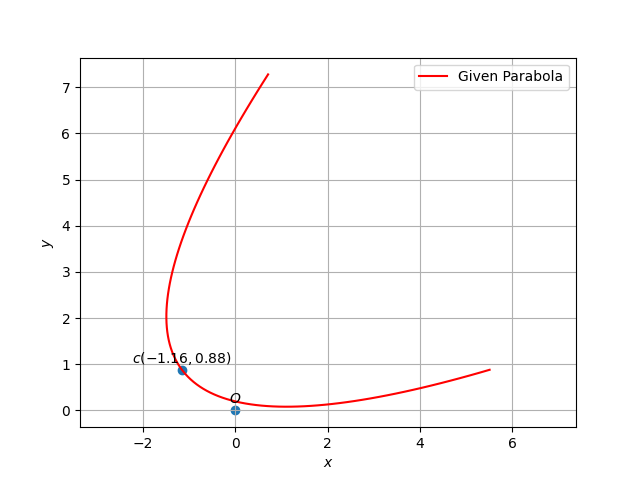
\includegraphics[width=\columnwidth]{./figs/parab/parab_gen.png}
    \caption{Parabola with the center c}
    \label{eq:conics/ex/solution/Fig:1}
\end{figure}
\end{enumerate}

\end{enumerate}

\section{Matrix Decompositions}
\subsection{QR Decomposition}
\renewcommand{\theequation}{\theenumi}
\begin{enumerate}[label=\thesubsection.\arabic*.,ref=\thesubsection.\theenumi]
\numberwithin{equation}{enumi}

\item Revisiting Problem \eqref{prob:line_gram_schmidt},
%
\begin{align}
\label{eq:decomp_qr_given}
{\alpha} = \myvec{3\\-1\\0},
 {\beta} = \myvec{2\\1\\-3}
\end{align}
%
we can express
\begin{align}
\begin{split}
\alpha = k_1\vec{u}_1 
\\
\beta = r_1\vec{u}_1 +k_2\vec{u}_2
\end{split}
\label{eq:decomp_gram}
\end{align}
%
where 
\begin{align}
k_1 = \norm{\alpha}, \vec{u}_1 = \frac{\vec{\alpha}}{k_1} 
\\
r_1 = \frac{\vec{u}_1^T\beta}{\norm{\vec{u}_1}^2}, 
\vec{u}_2 = \frac{\beta - r_1 \vec{u}_1}{\norm{\beta - r_1 \vec{u}_1}}
\\
k_2 = {\vec{u}_2^T\beta}
\end{align}
From \eqref{eq:decomp_gram}, 
\begin{align}
\myvec{\alpha & \beta } = \myvec{\vec{u}_1 & \vec{u}_2}\myvec{k_1 & r_1 \\ 0 & k_2} 
\end{align}
%
This is known as $\vec{Q}\vec{R}$ decomposition, where 
\begin{align}
\vec{R} = \myvec{k_1 & r_1 \\ 0 & k_2} 
\\
\vec{Q} = \myvec{\vec{u}_1 & \vec{u}_2}
\end{align}
%
Note that $\vec{R}$ is an upper triangular matrix and 
\begin{align}
\vec{Q}^T\vec{Q} = \vec{I}.
\end{align}
\item From \eqref{eq:decomp_qr_given},
\begin{align}
k_1 = \sqrt{10}, \vec{u}_1 = \frac{1}{\sqrt{10}} \myvec{3\\-1\\0},
\\
r_1 = \frac{1}{2}, \vec{u}_2 = \frac{1}{\sqrt{46}}\myvec{1\\3\\-6}
\\
k_2 = \sqrt{\frac{23}{2}}
\end{align}
Thus, we obtain the $\vec{Q}\vec{R}$ decompositon
\begin{align}
\myvec{
3 & 2
\\
-1 & 1
\\
0 & -3
}
=\myvec{
\frac{3}{\sqrt{10}} & \frac{1}{\sqrt{46}}
\\
\frac{-1}{\sqrt{10}} & \frac{3}{\sqrt{46}}
\\
0 & \frac{-6}{\sqrt{46}}
}
\myvec{
\sqrt{10}& \frac{1}{2}
\\
0&\sqrt{\frac{23}{2}}
}
\end{align}

\end{enumerate}

\subsection{Singular Value Decomposition}
\begin{enumerate}[label=\thesection.\arabic*,ref=\thesection.\theenumi]
\item Find the shortest distance between the lines\\  $\overrightarrow{r}=(\hat{i}+2\hat{j}+\hat{k})+\lambda(\hat{i}-\hat{j}+\hat{k})$ and \\$\overrightarrow{r}=2\hat{i}-\hat{j}-\hat{k}+\mu(2\hat{i}+\hat{j}+2\hat{k})$
\item Find the shortest distance between the lines\\
$ \frac{x+1}{7}=\frac{y+1}{-6}=\frac{z+1}{1}$ and $ \frac{x-3}{1}=\frac{y-5}{-2}=\frac{z-7}{1}$ 
    \solution
%		\iffalse
\documentclass[journal,12pt,twocolumn]{IEEEtran}
\usepackage{romannum}
\usepackage{float}
\usepackage{setspace}
\usepackage{gensymb}
\singlespacing
\usepackage[cmex10]{amsmath}
\usepackage{amsthm}
\usepackage{mathrsfs}
\usepackage{txfonts}
\usepackage{stfloats}
\usepackage{bm}
\usepackage{cite}
\usepackage{cases}
\usepackage{subfig}
\usepackage{longtable}
\usepackage{multirow}
\usepackage{enumitem}
\usepackage{mathtools}
\usepackage{steinmetz}
\usepackage{tikz}
\usepackage{circuitikz}
\usepackage{verbatim}
\usepackage{tfrupee}
\usepackage[breaklinks=true]{hyperref}
\usepackage{tkz-euclide}
\usetikzlibrary{calc,math}
\usepackage{listings}
    \usepackage{color}                                            %%
    \usepackage{array}                                            %%
    \usepackage{longtable}                                        %%
    \usepackage{calc}                                             %%
    \usepackage{multirow}                                         %%
    \usepackage{hhline}                                           %%
    \usepackage{ifthen}                                           %%
  %optionally (for landscape tables embedded in another document): %%
    \usepackage{lscape}     
\usepackage{multicol}
\usepackage{chngcntr}
\DeclareMathOperator*{\Res}{Res}
\renewcommand\thesection{\arabic{section}}
\renewcommand\thesubsection{\thesection.\arabic{subsection}}
\renewcommand\thesubsubsection{\thesubsection.\arabic{subsubsection}}

\renewcommand\thesectiondis{\arabic{section}}
\renewcommand\thesubsectiondis{\thesectiondis.\arabic{subsection}}
\renewcommand\thesubsubsectiondis{\thesubsectiondis.\arabic{subsubsection}}

% correct bad hyphenation here
\hyphenation{op-tical net-works semi-conduc-tor}
\def\inputGnumericTable{}                                 %%

\lstset{
frame=single, 
breaklines=true,
columns=fullflexible
}

\begin{document}


\newtheorem{theorem}{Theorem}[section]
\newtheorem{problem}{Problem}
\newtheorem{proposition}{Proposition}[section]
\newtheorem{lemma}{Lemma}[section]
\newtheorem{corollary}[theorem]{Corollary}
\newtheorem{example}{Example}[section]
\newtheorem{definition}[problem]{Definition}
\newcommand{\BEQA}{\begin{eqnarray}}
\newcommand{\EEQA}{\end{eqnarray}}
\newcommand{\define}{\stackrel{\triangle}{=}}

\bibliographystyle{IEEEtran}
\providecommand{\mbf}{\mathbf}
\providecommand{\pr}[1]{\ensuremath{\Pr\left(#1\right)}}
\providecommand{\qfunc}[1]{\ensuremath{Q\left(#1\right)}}
\providecommand{\sbrak}[1]{\ensuremath{{}\left[#1\right]}}
\providecommand{\lsbrak}[1]{\ensuremath{{}\left[#1\right.}}
\providecommand{\rsbrak}[1]{\ensuremath{{}\left.#1\right]}}
\providecommand{\brak}[1]{\ensuremath{\left(#1\right)}}
\providecommand{\lbrak}[1]{\ensuremath{\left(#1\right.}}
\providecommand{\rbrak}[1]{\ensuremath{\left.#1\right)}}
\providecommand{\cbrak}[1]{\ensuremath{\left\{#1\right\}}}
\providecommand{\lcbrak}[1]{\ensuremath{\left\{#1\right.}}
\providecommand{\rcbrak}[1]{\ensuremath{\left.#1\right\}}}
\theoremstyle{remark}
\newtheorem{rem}{Remark}
\newcommand{\sgn}{\mathop{\mathrm{sgn}}}
\providecommand{\abs}[1]{\left\vert#1\right\vert}
\providecommand{\res}[1]{\Res\displaylimits_{#1}} 
\providecommand{\norm}[1]{\left\lVert#1\right\rVert}
\providecommand{\mtx}[1]{\mathbf{#1}}
\providecommand{\mean}[1]{E\left[ #1 \right]}
\providecommand{\fourier}{\overset{\mathcal{F}}{ \rightleftharpoons}}
\providecommand{\system}{\overset{\mathcal{H}}{ \longleftrightarrow}}
\newcommand{\solution}{\noindent \textbf{Solution: }}
\newcommand{\cosec}{\,\text{cosec}\,}
\providecommand{\dec}[2]{\ensuremath{\overset{#1}{\underset{#2}{\gtrless}}}}
\newcommand{\myvec}[1]{\ensuremath{\begin{pmatrix}#1\end{pmatrix}}}
\newcommand{\mydet}[1]{\ensuremath{\begin{vmatrix}#1\end{vmatrix}}}
\numberwithin{equation}{subsection}
\makeatletter
\@addtoreset{figure}{problem}
\makeatother

\let\StandardTheFigure\thefigure
\let\vec\mathbf
\renewcommand{\thefigure}{\theproblem}



\def\putbox#1#2#3{\makebox[0in][l]{\makebox[#1][l]{}\raisebox{\baselineskip}[0in][0in]{\raisebox{#2}[0in][0in]{#3}}}}
     \def\rightbox#1{\makebox[0in][r]{#1}}
     \def\centbox#1{\makebox[0in]{#1}}
     \def\topbox#1{\raisebox{-\baselineskip}[0in][0in]{#1}}
     \def\midbox#1{\raisebox{-0.5\baselineskip}[0in][0in]{#1}}

\vspace{3cm}


\title{Question: 12.11.2.15}
\author{Nikam Pratik Balasaheb (EE21BTECH11037)}





% make the title area
\maketitle

\newpage

%\tableofcontents

\bigskip

\renewcommand{\thefigure}{\theenumi}
\renewcommand{\thetable}{\theenumi}

\section{Problem}
Find the shortest distance between the lines $\frac{x+1}{7} = \frac{y+1}{-6}=\frac{z+1}{1}$ and $\frac{x-3}{1} = \frac{y-5}{-2}=\frac{z-7}{1}$

\section{Solution}
\fi
 The given lines  can be written as
\begin{align}
\vec{x} &= \myvec{-1\\-1\\-1} + \lambda_1\myvec{7\\-6\\1}\\
\vec{x} &= \myvec{3\\5\\7} + \lambda_2\myvec{1\\-2\\1} \\
\vec{x_1} = \myvec{-1\\-1\\-1},\, \vec{x_2} &= \myvec{3\\5\\7}, \,\vec{m_1} = \myvec{7\\-6\\1}, \, \vec{m_2} = \myvec{1\\-2\\1}
\end{align}
%
We first check whether the given lines are skew. The lines 
\begin{align}
\vec{x} = \vec{x_1} + \lambda_1\vec{m_1},\, \vec{x} = \vec{x_2} + \lambda_2\vec{m_2} 
\label{eq:chapters/12/11/2/15/1}
\end{align}
intersect if
\begin{align}
\vec{M}{\lambda} &= \vec{x_2} - \vec{x_1}\\
\vec{M} &\triangleq \myvec{\vec{m_1} & \vec{m_2}} \\
\bm{\lambda} &\triangleq \myvec{\lambda_1\\-\lambda_2}\\
\end{align}
Here we have,
\begin{align}
\vec{M} = \myvec{7&1\\-6&-2\\1&1}\,
\vec{x_2} - \vec{x_1} = \myvec{4\\6\\8}
\end{align}
We check whether the equation \eqref{eq:chapters/12/11/2/15/2} has a solution
\begin{align}
\myvec{7&1\\-6&-2\\1&1}\bm{\lambda} = \myvec{4\\6\\8}
\label{eq:chapters/12/11/2/15/2}
\end{align}
the augmented matrix is given by,
\begin{align}
\myvec{7&1&\vrule&4\\-6&-2&\vrule&6\\1&1&\vrule&8}
\xleftrightarrow[R_3 \leftarrow R_3 - \frac{1}{7}R_1]{R_2 \leftarrow R_2 + \frac{6}{7}R_1}\\
\myvec{7&1&\vrule&4\\&&\vrule\\0&-\frac{8}{7}&\vrule&\frac{66}{7}\\&&\vrule\\0&\frac{6}{7}&\vrule&-\frac{52}{7}}
\xleftrightarrow{R_3 \leftarrow R_3 + \frac{3}{4}R_2}\\
\myvec{2&3&\vrule&1\\&&\vrule\\0&-\frac{7}{2}&\vrule&\frac{1}{2}\\&&\vrule\\0&0&\vrule&-\frac{5}{14}}
\end{align}
The rank of the matrix is 3. So the given lines are skew.
The closest points on two skew lines defined by \eqref{eq:chapters/12/11/2/15/1} are given by 
\begin{align}
\vec{M}^\top \vec{M}\bm{\lambda} &= \vec{M}^\top\brak{\vec{x_2}-\vec{x_1}}\\
\implies \myvec{7&-6&1\\1&-2&1} \myvec{7&1\\-6&-2\\1&1}\bm{\lambda} &= \myvec{7&-6&1\\1&-2&1} \myvec{4\\6\\8}\\
\implies \myvec{86&20\\20&6}\bm{\lambda} &= \myvec{0\\0}
\label{eq:chapters/12/11/2/15/3}
\end{align}
The augmented matrix of the above equation \eqref{eq:chapters/12/11/2/15/3} is given by,
\begin{align}
\myvec{86&20&\vrule&0\\20&6&\vrule&0}
\xleftrightarrow{R_2 \leftarrow R_2 - \frac{10}{43}R_1}
\myvec{86&20&\vrule&0 \\&&\vrule\\ 0&\frac{58}{43}&\vrule&0}
\xleftrightarrow[R_2 \leftarrow \frac{43}{58}R_2]{R_1 \leftarrow \frac{1}{86} \brak{R_1 - \frac{430}{29}R_2}}\\
\myvec{1&0&\vrule&0 \\&&\vrule\\ 0&1&\vrule&0}
\end{align}
yielding
\begin{align}
\myvec{\lambda_1\\-\lambda_2} &= \myvec{0\\0}
\end{align}
The closest points $\vec{A}$ on line $l_1$ and $\vec{B}$ on line $l_2$ are given by,
\begin{align}
\vec{A} &= \vec{x_1} + \lambda_1\vec{m_1}
= \myvec{-1\\-1\\-1}\\
\vec{B} &= \vec{x_2} + \lambda_2\vec{m_2}
= \myvec{3\\5\\7}
\end{align}
The minimum distance between the lines is given by
\begin{align}
\norm{\vec{B}-\vec{A}} &= \norm{\myvec{4\\6\\8}}
= 2\sqrt{29}
\end{align}
%
\begin{figure}[!ht]
\centering
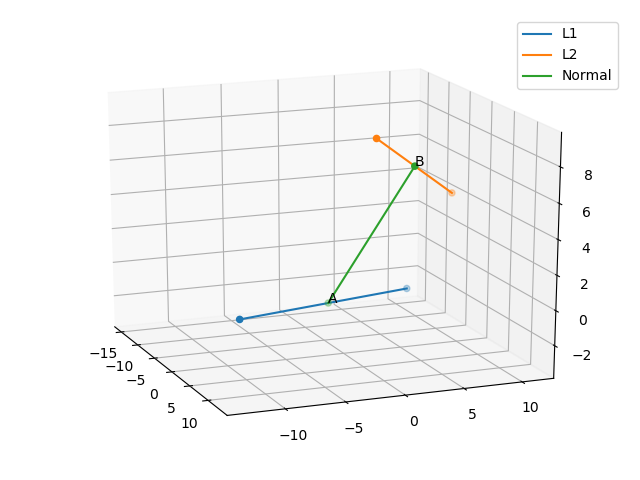
\includegraphics[width=\columnwidth]{chapters/12/11/2/15/figs/Figure_1.png}
\caption{}
\label{fig:chapters/12/11/2/15/}
\end{figure}


    \item Find the shortest distance between the lines whose vector equations are
    \begin{align}
        \vec{x} = \myvec{1\\2\\3} + \lambda_1\myvec{1\\-3\\2}
        \label{eq:chapters/12/11/2/16/L1/svd}
    \end{align}
    and
    \begin{align}
        \vec{x} = \myvec{4\\5\\6} + \lambda_2\myvec{2\\3\\1}
        \label{eq:chapters/12/11/2/16/L2/svd}
    \end{align}
    \solution
		\iffalse
\documentclass[journal,12pt,twocolumn]{IEEEtran}
\usepackage{setspace}
\usepackage{gensymb}
\usepackage{xcolor}
\usepackage{caption}
\singlespacing
\usepackage{siunitx}
\usepackage[cmex10]{amsmath}
\usepackage{mathtools}
\usepackage{hyperref}
\usepackage{amsthm}
\usepackage{mathrsfs}
\usepackage{txfonts}
\usepackage{stfloats}
\usepackage{cite}
\usepackage{cases}
\usepackage{subfig}
\usepackage{longtable}
\usepackage{multirow}
\usepackage{enumitem}
\usepackage{bm}
\usepackage{mathtools}
\usepackage{listings}
\usepackage{tikz}
\usetikzlibrary{shapes,arrows,positioning}
\usepackage{circuitikz}
\renewcommand{\vec}[1]{\boldsymbol{\mathbf{#1}}}
\DeclareMathOperator*{\Res}{Res}
\renewcommand\thesection{\arabic{section}}
\renewcommand\thesubsection{\thesection.\arabic{subsection}}
\renewcommand\thesubsubsection{\thesubsection.\arabic{subsubsection}}

\renewcommand\thesectiondis{\arabic{section}}
\renewcommand\thesubsectiondis{\thesectiondis.\arabic{subsection}}
\renewcommand\thesubsubsectiondis{\thesubsectiondis.\arabic{subsubsection}}
\hyphenation{op-tical net-works semi-conduc-tor}

\lstset{
language=Python,
frame=single, 
breaklines=true,
columns=fullflexible
}
\begin{document}
\theoremstyle{definition}
\newtheorem{theorem}{Theorem}[section]
\newtheorem{problem}{Problem}
\newtheorem{proposition}{Proposition}[section]
\newtheorem{lemma}{Lemma}
\newtheorem{corollary}[theorem]{Corollary}
\newtheorem{example}{Example}[section]
\newtheorem{definition}{Definition}[section]
\newcommand{\BEQA}{\begin{eqnarray}}
\newcommand{\EEQA}{\end{eqnarray}}
\newcommand{\define}{\stackrel{\triangle}{=}}
\newcommand{\myvec}[1]{\ensuremath{\begin{pmatrix}#1\end{pmatrix}}}
\newcommand{\mydet}[1]{\ensuremath{\begin{vmatrix}#1\end{vmatrix}}}
\bibliographystyle{IEEEtran}
\providecommand{\nCr}[2]{\,^{#1}C_{#2}} % nCr
\providecommand{\nPr}[2]{\,^{#1}P_{#2}} % nPr
\providecommand{\mbf}{\mathbf}
\providecommand{\pr}[1]{\ensuremath{\Pr\left(#1\right)}}
\providecommand{\chr}[1]{\ensuremath{\textrm{char}\left(#1\right)}}
\providecommand{\qfunc}[1]{\ensuremath{Q\left(#1\right)}}
\providecommand{\sbrak}[1]{\ensuremath{{}\left[#1\right]}}
\providecommand{\lsbrak}[1]{\ensuremath{{}\left[#1\right.}}
\providecommand{\rsbrak}[1]{\ensuremath{{}\left.#1\right]}}
\providecommand{\brak}[1]{\ensuremath{\left(#1\right)}}
\providecommand{\lbrak}[1]{\ensuremath{\left(#1\right.}}
\providecommand{\rbrak}[1]{\ensuremath{\left.#1\right)}}
\providecommand{\cbrak}[1]{\ensuremath{\left\{#1\right\}}}
\providecommand{\lcbrak}[1]{\ensuremath{\left\{#1\right.}}
\providecommand{\rcbrak}[1]{\ensuremath{\left.#1\right\}}}
\theoremstyle{remark}
\newtheorem{rem}{Remark}
\newcommand{\sgn}{\mathop{\mathrm{sgn}}}
\newcommand{\rect}{\mathop{\mathrm{rect}}}
\newcommand{\sinc}{\mathop{\mathrm{sinc}}}
\providecommand{\abs}[1]{\left\vert#1\right\vert}
\providecommand{\res}[1]{\Res\displaylimits_{#1}} 
\providecommand{\norm}[1]{\left\Vert#1\right\Vert}
\providecommand{\mtx}[1]{\mathbf{#1}}
\providecommand{\mean}[1]{E\left[ #1 \right]}
\providecommand{\fourier}{\overset{\mathcal{F}}{ \rightleftharpoons}}
\providecommand{\ztrans}{\overset{\mathcal{Z}}{ \rightleftharpoons}}
\providecommand{\system}[1]{\overset{\mathcal{#1}}{ \longleftrightarrow}}
\newcommand{\solution}{\noindent \textbf{Solution: }}
\providecommand{\dec}[2]{\ensuremath{\overset{#1}{\underset{#2}{\gtrless}}}}
\let\StandardTheFigure\thefigure
\def\putbox#1#2#3{\makebox[0in][l]{\makebox[#1][l]{}\raisebox{\baselineskip}[0in][0in]{\raisebox{#2}[0in][0in]{#3}}}}
     \def\rightbox#1{\makebox[0in][r]{#1}}
     \def\centbox#1{\makebox[0in]{#1}}
     \def\topbox#1{\raisebox{-\baselineskip}[0in][0in]{#1}}
     \def\midbox#1{\raisebox{-0.5\baselineskip}[0in][0in]{#1}}

\vspace{3cm}
\title{Line Assignment}
\author{Gautam Singh}
\maketitle
\bigskip

\begin{abstract}
    This document contains a general solution to Question 16 of 
    Exercise 2 in Chapter 11 of the class 12 NCERT textbook.
\end{abstract}

\begin{enumerate}
    \item Find the shortest distance between the lines whose vector equations are
    \begin{align}
        L_1: \vec{x} = \vec{x_1} + \lambda_1\vec{m_1} \label{eq:chapters/12/11/2/16/svd/L1} \\
        L_2: \vec{x} = \vec{x_2} + \lambda_2\vec{m_2} \label{eq:chapters/12/11/2/16/svd/L2}
    \end{align}

    \solution 
\fi
		Let $\vec{A}$ and $\vec{B}$ be points on lines $L_1$ and $L_2$
    respectively such that $AB$ is normal to both lines. Define
    \begin{align}
        \vec{M} &\triangleq \myvec{\vec{m_1} & \vec{m_2}} \label{eq:chapters/12/11/2/16/svd/M-def} \\
        \vec{\lambda} &\triangleq \myvec{\lambda_1\\-\lambda_2} \label{eq:chapters/12/11/2/16/svd/lambda-def} \\
        \vec{x} &\triangleq \vec{x_2} - \vec{x_1} \label{eq:chapters/12/11/2/16/svd/x-def}
    \end{align}
    Then, we have the following equations:
    \begin{align}
        \vec{A} = \vec{x_1} + \lambda_1\vec{m_1} \label{eq:chapters/12/11/2/16/svd/A-def} \\
        \vec{B} = \vec{x_2} + \lambda_2\vec{m_2} \label{eq:chapters/12/11/2/16/svd/B-def}
    \end{align}
    From \eqref{eq:chapters/12/11/2/16/svd/A-def} and \eqref{eq:chapters/12/11/2/16/svd/B-def}, define the real-valued function
    $f$ as
    \begin{align}
        f\brak{\vec{\lambda}} &\triangleq \norm{\vec{A}-\vec{B}}^2 \\
                              &= \norm{\vec{M}\vec{\lambda}-\vec{x}}^2 \\
                              &= \brak{\vec{M\lambda}-\vec{x}}^\top\brak{\vec{M\lambda}-\vec{x}} \\
                              &= \vec{\lambda}^\top\brak{\vec{M}^\top\vec{M}}\vec{\lambda} - 2\vec{x}^\top\vec{M\lambda} + \norm{\vec{x}}^2
        \label{eq:chapters/12/11/2/16/svd/f-def}
    \end{align}
    From \eqref{eq:chapters/12/11/2/16/svd/f-def}, we see that $f$ is quadratic in $\vec{\lambda}$.

    We now prove a useful lemma here.
    \begin{lemma}
        The quadratic form
        \begin{align}
            q\brak{\vec{x}} \triangleq \vec{x}^\top\vec{Ax} + \vec{b}^\top\vec{x} + c
            \label{eq:chapters/12/11/2/16/svd/quad-x}
        \end{align}
        is convex iff $\vec{A}$ is positive semi-definite.
    \end{lemma}
    \begin{proof}
        Consider two points $\vec{x_1}$ and $\vec{x_2}$, and a real constant
        $0 \le \mu \le 1$. Then,
        \begin{align}
            &\mu f\brak{\vec{x_1}} + \brak{1-\mu}f\brak{\vec{x_2}} - f\brak{\mu\vec{x_1}+\brak{1-\mu}\vec{x_2}} \nonumber \\
            &= \brak{\mu-\mu^2}\vec{x_1}^\top\vec{Ax_1} + \brak{1-\mu-\brak{1-\mu}^2}\vec{x_2}^\top\vec{Ax_2} \nonumber \\
            &- 2\mu\brak{1-\mu}\vec{x_1}^\top\vec{Ax_2} \\
            &= \mu\brak{1-\mu}\brak{\vec{x_1}^\top\vec{Ax_1}-2\vec{x_1}^\top\vec{Ax_2}+\vec{x_2}^\top\vec{Ax_2}} \\
            &= \mu\brak{1-\mu}\brak{\vec{x_1}-\vec{x_2}}^\top\vec{A}\brak{\vec{x_1}-\vec{x_2}}
            \label{eq:chapters/12/11/2/16/svd/psd-iff}
        \end{align}
        Since $\vec{x_1}$ and $\vec{x_2}$ are arbitrary, it follows from 
        \eqref{eq:chapters/12/11/2/16/svd/psd-iff} that
        \begin{align}
            \mu f\brak{\vec{x_1}} + \brak{1-\mu}f\brak{\vec{x_2}} \ge f\brak{\mu\vec{x_1}+\brak{1-\mu}\vec{x_2}}
        \end{align}
        iff $\vec{A}$ is positive semi-definite, as required.
    \end{proof}
    Using the above lemma, we show that $f$ is convex by showing that 
    $\vec{M}^\top\vec{M}$ is positive semi-definite. Indeed, for any 
    $\vec{p} \triangleq \myvec{x\\y}$,
    \begin{align}
        \vec{p}^\top\vec{M}^\top\vec{Mp} = \norm{\vec{Mp}}^2 \ge 0
        \label{eq:chapters/12/11/2/16/svd/psd}
    \end{align}
    and thus, $f$ is convex.

    We need to minimize $f$ as a function of $\vec{\lambda}$.
    Differentiating \eqref{eq:chapters/12/11/2/16/svd/f-def} using the chain rule,
    \begin{align}
        \frac{df\brak{\vec{\lambda}}}{d\vec{\lambda}} &= \vec{M}^\top\brak{\vec{M\lambda}-\vec{x}}+\vec{M}\brak{\vec{M\lambda}-\vec{x}}^\top \\
                                                      &= 2\vec{M}^\top\brak{\vec{M\lambda}-\vec{x}}
        \label{eq:chapters/12/11/2/16/svd/vec-min}
    \end{align}
    Setting \eqref{eq:chapters/12/11/2/16/svd/vec-min} to zero gives the equation
    \begin{align}
        \vec{M}^\top\vec{M\lambda} = \vec{M}^\top\vec{x}
        \label{eq:chapters/12/11/2/16/svd/vec-eqn}
    \end{align}
    We use singular value decomposition here. Let
    \begin{align}
        \vec{M} = \vec{U\Sigma V}^\top
        \label{eq:chapters/12/11/2/16/svd/M-svd}
    \end{align}
    where $\vec{U}, \vec{V}$ are orthogonal and $\vec{\Sigma}$ is diagonal with
    nonnegative diagonal entries. Substituting in \eqref{eq:chapters/12/11/2/16/svd/vec-eqn},
    \begin{align}
        \vec{V\Sigma U}^\top\vec{U\Sigma V}^\top\vec{\lambda} = \vec{V\Sigma U}^\top\vec{x} \\
        \implies \vec{V\Sigma}^2\vec{V}^\top\vec{\lambda} = \vec{V\Sigma U}^\top\vec{x} \\
        \implies \vec{\lambda} = \brak{\vec{V\Sigma}^2\vec{V}^\top}^{-1}\vec{V\Sigma U}^\top\vec{x} \\
        \implies \vec{\lambda} = \vec{V\Sigma}^{-2}\vec{V}^\top\vec{V\Sigma U}^\top\vec{x} \\
        \implies \vec{\lambda} = \vec{V\Sigma}^{-1}\vec{U}^\top\vec{x} \label{eq:chapters/12/11/2/16/svd/lambda-sol}
    \end{align}
    where $\vec{\Sigma}^{-1}$ is obtained by inverting the nonzero elements of
    $\vec{\Sigma}$. Thus, the shortest distance is given by using \eqref{eq:chapters/12/11/2/16/svd/M-svd}
    and \eqref{eq:chapters/12/11/2/16/svd/lambda-sol} in \eqref{eq:chapters/12/11/2/16/svd/f-def}, and is given by
    \begin{align}
        d = \norm{\brak{\vec{U}\brak{\vec{\Sigma\Sigma}^{-1}}\vec{U}^\top-\vec{I}}\vec{x}}
        \label{eq:chapters/12/11/2/16/svd/min-sol}
    \end{align}
    For this problem,
    \begin{align}
        \vec{x} = \vec{x_2} - \vec{x_1} = \myvec{3\\3\\3} \\
        \vec{M} = \myvec{\vec{m_1} & \vec{m_2}} = \myvec{1&2\\-3&3\\2&1} 
    \end{align}
    Thus,
    \begin{align}
        \vec{M}^\top\vec{M} = \myvec{1&-3&2\\2&3&1}\myvec{1&2\\-3&3\\2&1} = \myvec{14&-5\\-5&14} \\
        \vec{MM}^\top = \myvec{1&2\\-3&3\\2&1}\myvec{1&-3&2\\2&3&1} = \myvec{5&3&4\\3&18&-3\\4&-3&5}
    \end{align}
    We perform the eigendecompositions for each matrix and bring them into the form
    \begin{align}
        \vec{MM}^\top &= \vec{P_1D_1P_1}^\top \label{eq:chapters/12/11/2/16/svd/decomp-1} \\
        \vec{M}^\top\vec{M} &= \vec{P_2D_2P_2}^\top \label{eq:chapters/12/11/2/16/svd/decomp-2}
    \end{align}
    \begin{enumerate}
        \item For $\vec{MM}^\top$, the characteristic polynomial is
        \begin{align}
		\text{char}{\vec{MM}^\top} &= \mydet{x-5&-3&-4\\-3&x-18&3\\-4&3&x-5} \\
                                      &= x\brak{x-9}\brak{x-19}
                                      \label{eq:chapters/12/11/2/16/svd/char-2}
        \end{align}
        Thus, the eigenvalues are given by
        \begin{align}
            \lambda_1 = 19,\ \lambda_2 = 9,\ \lambda_3 = 0
        \end{align}
        For $\lambda_1$, the augmented matrix formed from the 
        eigenvalue-eigenvector equation is
        \begin{align}
            &\myvec{-14&3&4&0\\3&-1&-3&0\\4&-3&-14&0} \nonumber \\
            &\xleftrightarrow[]{R_1 \leftarrow \frac{R_1+R_3}{-10}} \myvec{1&0&1&0\\3&-1&-3&0\\4&-3&-14&0} \\
            &\xleftrightarrow[]{R_2 \leftarrow -R_2+3R_1} \myvec{1&0&1&0\\0&1&6&0\\4&-3&-14&0} \\
            &\xleftrightarrow[]{R_3 \leftarrow R_3-4R_1} \myvec{1&0&1&0\\0&-1&-6&0\\0&-3&-18&0} \\
            &\xleftrightarrow[]{R_3 \leftarrow R_3-3R_2} \myvec{1&0&1&0\\0&-1&-6&0\\0&0&0&0}
        \end{align}
        Hence, the normalized eigenvector is
        \begin{align}
            \vec{p_1} = \frac{1}{\sqrt{38}}\myvec{-1\\-6\\1}
        \end{align}
        For $\lambda_2$, the augmented matrix formed from the 
        eigenvalue-eigenvector equation is
        \begin{align}
            &\myvec{-4&3&4&0\\3&9&-3&0\\4&3&-4&0} \nonumber \\
            &\xleftrightarrow[]{R_3 \leftarrow R_1+R_3} \myvec{-4&3&4&0\\3&9&-3&0\\0&0&0&0} \\
            &\xleftrightarrow[]{R_2 \leftarrow \frac{4R_2+3R_1}{45}} \myvec{-4&3&4&0\\0&1&0&0\\0&0&0&0} \\
            &\xleftrightarrow[]{R_1 \leftarrow \frac{R_1-3R_2}{-4}} \myvec{1&0&-1&0\\0&1&0&0\\0&0&0&0}
        \end{align}
        Hence, the normalized eigenvector is
        \begin{align}
            \vec{p_2} = \frac{1}{\sqrt{2}}\myvec{1\\0\\1}
        \end{align}
        For $\lambda_3$, the augmented matrix formed from the 
        eigenvalue-eigenvector equation is
        \begin{align}
            &\myvec{5&3&4&0\\3&18&-3&0\\4&-3&5&0} \nonumber \\ 
            &\xleftrightarrow[]{R_1 \leftarrow \frac{R_1+R_3}{9}} \myvec{1&0&1&0\\3&18&-3&0\\4&-3&5&0} \\
            &\xleftrightarrow[]{R_2 \leftarrow R_2-3R_1} \myvec{1&0&1&0\\0&18&-6&0\\4&-3&5&0} \\
            &\xleftrightarrow[]{R_3 \leftarrow R_3-4R_1} \myvec{1&0&1&0\\0&18&-6&0\\0&-3&1&0} \\
            &\xleftrightarrow[]{R_2 \leftarrow \frac{R_2}{6}} \myvec{1&0&1&0\\0&3&-1&0\\0&-3&1&0} \\
            &\xleftrightarrow[]{R_3 \leftarrow R_3+R_2} \myvec{1&0&1&0\\0&3&-1&0\\0&0&0&0}
        \end{align}
        Hence, the normalized eigenvector is
        \begin{align}
            \vec{p_3} = \frac{1}{\sqrt{19}}\myvec{-3\\1\\3}
        \end{align}
        Using \eqref{eq:chapters/12/11/2/16/svd/decomp-1}, we see that
        \begin{align}
            \vec{P_1} = \myvec{-\frac{1}{\sqrt{38}}&\frac{1}{\sqrt{2}}&-\frac{3}{\sqrt{19}}\\-\frac{6}{\sqrt{38}}&0&\frac{1}{\sqrt{19}}\\\frac{1}{\sqrt{38}}&-\frac{1}{\sqrt{2}}&\frac{3}{\sqrt{19}}} \\
            \vec{D_1} = \myvec{19&0&0\\0&9&0\\0&0&0}
            \label{eq:chapters/12/11/2/16/svd/eig-params-1}
        \end{align}
        \item For $\vec{M}^\top\vec{M}$, the characteristic polynomial is
        \begin{align}
		\text{char}{\vec{M}^\top\vec{M}} &= \mydet{x-14&5\\5&x-14} \\
                                      &= \brak{x-9}\brak{x-19}
%                                      \label{eq:chapters/12/11/2/16/svd/char-1}
        \end{align}
        Thus, the eigenvalues are given by
        \begin{align}
            \lambda_1 = 19,\ \lambda_2 = 9
        \end{align}
        For $\lambda_1$, the augmented matrix formed from the 
        eigenvalue-eigenvector equation is
        \begin{align}
            \myvec{-5&-5&0\\-5&-5&0} &\xleftrightarrow[]{R_1 \leftarrow R_1-R_2} \myvec{0&0&0\\-5&-5&0}
        \end{align}
        Hence, the normalized eigenvector is
        \begin{align}
            \vec{p_1} = \frac{1}{\sqrt{2}}\myvec{1\\-1}
        \end{align}
        For $\lambda_2$, the augmented matrix formed from the 
        eigenvalue-eigenvector equation is
        \begin{align}
            \myvec{5&-5&0\\-5&5&0} &\xleftrightarrow[]{R_1 \leftarrow R_1+R_2} \myvec{0&0&0\\5&-5&0}
        \end{align}
        Hence, the normalized eigenvector is
        \begin{align}
            \vec{p_2} = \frac{1}{\sqrt{2}}\myvec{1\\1}
        \end{align}
        Thus, from \eqref{eq:chapters/12/11/2/16/svd/decomp-2},
        \begin{align}
            \vec{P_2} = \myvec{\frac{1}{\sqrt{2}}&-\frac{1}{\sqrt{2}}\\\frac{1}{\sqrt{2}}&\frac{1}{\sqrt{2}}},\ \vec{D_2} = \myvec{9&0\\0&19}
            \label{eq:chapters/12/11/2/16/svd/eig-params-2}
        \end{align}
    \end{enumerate}
    Therefore, from \eqref{eq:chapters/12/11/2/16/svd/M-svd},
    \begin{align}
        \vec{U} &= \vec{P_1} \\ 
        \vec{V} &= \vec{P_2} \\
        \vec{\Sigma} &= \myvec{\sqrt{19}&0\\0&3\\0&0}
        \label{eq:chapters/12/11/2/16/svd/svd-params}
    \end{align}
    and substituting into \eqref{eq:chapters/12/11/2/16/svd/lambda-sol}, we get
    \begin{align}
        \vec{\lambda} = \frac{1}{19}\myvec{10\\28}
    \end{align}
    which agrees with earlier solutions as well.
    \iffalse
    The Python code
    \texttt{codes/svd.py} plots 
    \fi
    See Fig. \ref{fig:chapters/12/11/2/16/svd/svd} depicting the situation.
    \begin{figure}[!ht]
        \centering
        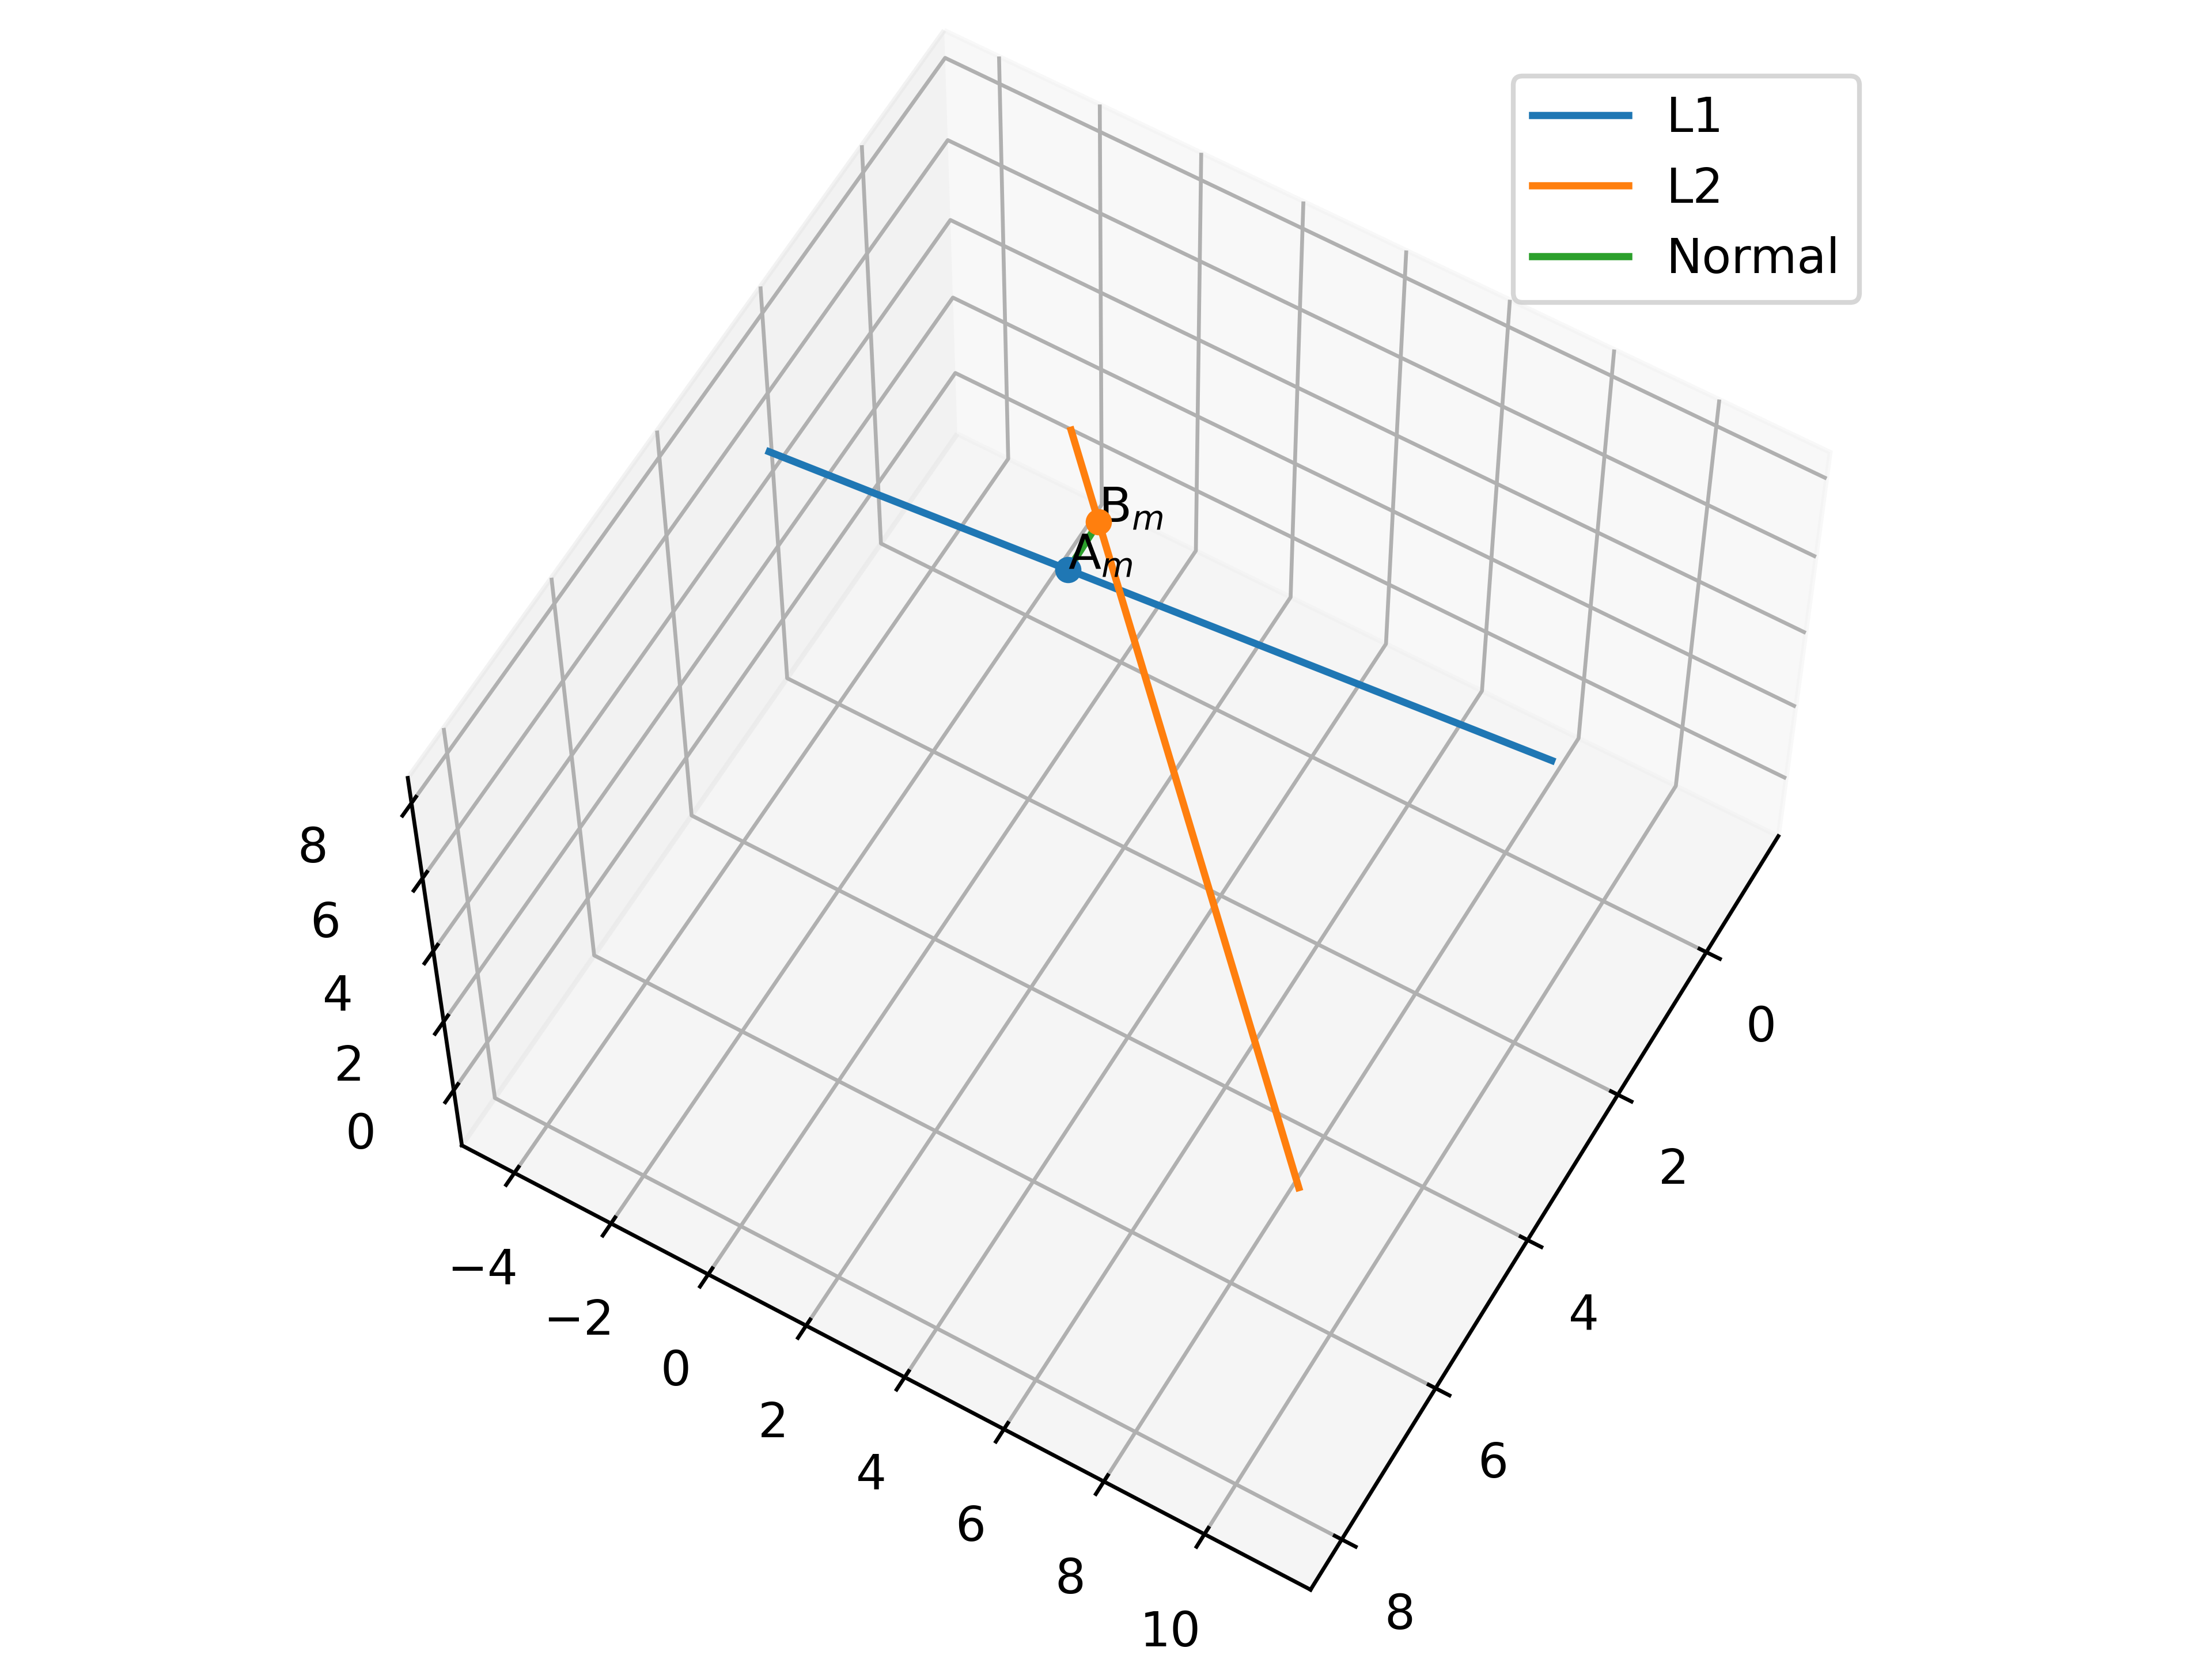
\includegraphics[width=\columnwidth]{chapters/12/11/2/16/svd/figs/skew_svd.png}
        \caption{Finding the shortest distance between two lines using SVD.}
        \label{fig:chapters/12/11/2/16/svd/svd}
    \end{figure}

\item Find the shortest distance between the lines $l_1$ and $l_2$ whose vector equations are ${\overrightarrow{r} = \hat{i}+\hat{j}+\lambda(2\hat{i}-\hat{j}+\hat{k})}$ and ${\overrightarrow{r} = 2\hat{i}+\hat{j}-\hat{k}+\mu(3\hat{i}-5\hat{j}+2\hat{k})}$.
\\
    \solution
		\iffalse
\documentclass[journal,12pt,twocolumn]{IEEEtran}
\usepackage{romannum}
\usepackage{float}
\usepackage{setspace}
\usepackage{gensymb}
\singlespacing
\usepackage[cmex10]{amsmath}
\usepackage{amsthm}
\usepackage{mathrsfs}
\usepackage{txfonts}
\usepackage{stfloats}
\usepackage{bm}
\usepackage{cite}
\usepackage{cases}
\usepackage{subfig}
\usepackage{longtable}
\usepackage{multirow}
\usepackage{enumitem}
\usepackage{mathtools}
\usepackage{steinmetz}
\usepackage{tikz}
\usepackage{circuitikz}
\usepackage{verbatim}
\usepackage{tfrupee}
\usepackage[breaklinks=true]{hyperref}
\usepackage{tkz-euclide}
\usetikzlibrary{calc,math}
\usepackage{listings}
    \usepackage{color}                                            %%
    \usepackage{array}                                            %%
    \usepackage{longtable}                                        %%
    \usepackage{calc}                                             %%
    \usepackage{multirow}                                         %%
    \usepackage{hhline}                                           %%
    \usepackage{ifthen}                                           %%
  %optionally (for landscape tables embedded in another document): %%
    \usepackage{lscape}     
\usepackage{multicol}
\usepackage{chngcntr}
\DeclareMathOperator*{\Res}{Res}
\renewcommand\thesection{\arabic{section}}
\renewcommand\thesubsection{\thesection.\arabic{subsection}}
\renewcommand\thesubsubsection{\thesubsection.\arabic{subsubsection}}

\renewcommand\thesectiondis{\arabic{section}}
\renewcommand\thesubsectiondis{\thesectiondis.\arabic{subsection}}
\renewcommand\thesubsubsectiondis{\thesubsectiondis.\arabic{subsubsection}}

% correct bad hyphenation here
\hyphenation{op-tical net-works semi-conduc-tor}
\def\inputGnumericTable{}                                 %%

\lstset{
frame=single, 
breaklines=true,
columns=fullflexible
}

\begin{document}


\newtheorem{theorem}{Theorem}[section]
\newtheorem{problem}{Problem}
\newtheorem{proposition}{Proposition}[section]
\newtheorem{lemma}{Lemma}[section]
\newtheorem{corollary}[theorem]{Corollary}
\newtheorem{example}{Example}[section]
\newtheorem{definition}[problem]{Definition}
\newcommand{\BEQA}{\begin{eqnarray}}
\newcommand{\EEQA}{\end{eqnarray}}
\newcommand{\define}{\stackrel{\triangle}{=}}

\bibliographystyle{IEEEtran}
\providecommand{\mbf}{\mathbf}
\providecommand{\pr}[1]{\ensuremath{\Pr\left(#1\right)}}
\providecommand{\qfunc}[1]{\ensuremath{Q\left(#1\right)}}
\providecommand{\sbrak}[1]{\ensuremath{{}\left[#1\right]}}
\providecommand{\lsbrak}[1]{\ensuremath{{}\left[#1\right.}}
\providecommand{\rsbrak}[1]{\ensuremath{{}\left.#1\right]}}
\providecommand{\brak}[1]{\ensuremath{\left(#1\right)}}
\providecommand{\lbrak}[1]{\ensuremath{\left(#1\right.}}
\providecommand{\rbrak}[1]{\ensuremath{\left.#1\right)}}
\providecommand{\cbrak}[1]{\ensuremath{\left\{#1\right\}}}
\providecommand{\lcbrak}[1]{\ensuremath{\left\{#1\right.}}
\providecommand{\rcbrak}[1]{\ensuremath{\left.#1\right\}}}
\theoremstyle{remark}
\newtheorem{rem}{Remark}
\newcommand{\sgn}{\mathop{\mathrm{sgn}}}
\providecommand{\abs}[1]{\left\vert#1\right\vert}
\providecommand{\res}[1]{\Res\displaylimits_{#1}} 
\providecommand{\norm}[1]{\left\lVert#1\right\rVert}
\providecommand{\mtx}[1]{\mathbf{#1}}
\providecommand{\mean}[1]{E\left[ #1 \right]}
\providecommand{\fourier}{\overset{\mathcal{F}}{ \rightleftharpoons}}
\providecommand{\system}{\overset{\mathcal{H}}{ \longleftrightarrow}}
\newcommand{\solution}{\noindent \textbf{Solution: }}
\newcommand{\cosec}{\,\text{cosec}\,}
\providecommand{\dec}[2]{\ensuremath{\overset{#1}{\underset{#2}{\gtrless}}}}
\newcommand{\myvec}[1]{\ensuremath{\begin{pmatrix}#1\end{pmatrix}}}
\newcommand{\mydet}[1]{\ensuremath{\begin{vmatrix}#1\end{vmatrix}}}
\numberwithin{equation}{subsection}
\makeatletter
\@addtoreset{figure}{problem}
\makeatother

\let\StandardTheFigure\thefigure
\let\vec\mathbf
\renewcommand{\thefigure}{\theproblem}



\def\putbox#1#2#3{\makebox[0in][l]{\makebox[#1][l]{}\raisebox{\baselineskip}[0in][0in]{\raisebox{#2}[0in][0in]{#3}}}}
     \def\rightbox#1{\makebox[0in][r]{#1}}
     \def\centbox#1{\makebox[0in]{#1}}
     \def\topbox#1{\raisebox{-\baselineskip}[0in][0in]{#1}}
     \def\midbox#1{\raisebox{-0.5\baselineskip}[0in][0in]{#1}}

\vspace{3cm}


\title{Assignment 1}
\author{Jaswanth Chowdary Madala}





% make the title area
\maketitle

\newpage

%\tableofcontents

\bigskip

\renewcommand{\thefigure}{\theenumi}
\renewcommand{\thetable}{\theenumi}

\begin{enumerate}
\item Find the shortest distance between the lines $l_1$ and $l_2$ whose vector equations are ${\overrightarrow{r} = \hat{i}+\hat{j}+\lambda(2\hat{i}-\hat{j}+\hat{k})}$ and ${\overrightarrow{r} = 2\hat{i}+\hat{j}-\hat{k}+\mu(3\hat{i}-5\hat{j}+2\hat{k})}$

\textbf{Solution:} 
\fi
The shortest distance between the lines whose vector equations are
\begin{align}
L_1: \vec{x} = \vec{x_1} + \lambda_1\vec{m_1} \label{eq:chapters/12/11/2/311/svd/1} \\
L_2: \vec{x} = \vec{x_2} + \lambda_2\vec{m_2} \label{eq:chapters/12/11/2/311/svd/2}
\end{align}
is given by,
\begin{align}
d = \norm{\brak{\vec{U}\brak{\vec{\Sigma\Sigma}^{-1}}\vec{U}^\top-\vec{I}}\vec{x}}
\end{align}
with the parameter $\lambda$ given by
\begin{align}
\bm{\lambda} = \vec{V\Sigma}^{-1}\vec{U}^\top\vec{x} \label{eq:chapters/12/11/2/311/svd/lambda-sol}
\end{align}
where
\begin{align}
\vec{M} &\triangleq \myvec{\vec{m_1} & \vec{m_2}} \label{eq:chapters/12/11/2/311/svd/3}\\
\bm{\lambda} &\triangleq \myvec{\lambda_1\\-\lambda_2}\label{eq:chapters/12/11/2/311/svd/4} \\
\vec{x} &\triangleq \vec{x_2} - \vec{x_1} \label{eq:chapters/12/11/2/311/svd/5}
\end{align}

We use singular value decomposition of the matrix $\vec{M}$
\begin{align}
\vec{M} = \vec{U\Sigma V}^\top \label{eq:chapters/12/11/2/311/svd/6}
\end{align}
where $\vec{U}, \vec{V}$ are orthogonal and $\vec{\Sigma}$ is diagonal with nonnegative diagonal entries.

\begin{enumerate}
\item In this problem we have the lines $l_1$ and $l_2$ as
\begin{align}
\vec{x} &= \myvec{1\\1\\0} + \lambda_1\myvec{2\\-1\\1}\\
\vec{x} &= \myvec{2\\1\\-1} + \lambda_2\myvec{3\\-5\\2}
\end{align}

We first need to check whether the given lines are skew.
The lines \eqref{eq:chapters/12/11/2/311/svd/1}, \eqref{eq:chapters/12/11/2/311/svd/2} intersect if
\begin{align}
\vec{M}\bm{\lambda} &= \vec{x_2} - \vec{x_1}
\end{align}
Here we have,
\begin{align}
\vec{M} &= \myvec{2&3\\-1&-5\\1&2} \label{eq:chapters/12/11/2/311/svd/M}\\
\vec{x} = \vec{x_2} - \vec{x_1} &= \myvec{1\\0\\-1} \label{eq:chapters/12/11/2/311/svd/x}
\end{align}
We check whether the equation \eqref{eq:chapters/12/11/2/311/svd/7} has a solution
\begin{align}
\myvec{2&3\\-1&-5\\1&2}\bm{\lambda} = \myvec{1\\0\\-1}
\label{eq:chapters/12/11/2/311/svd/7}
\end{align}
the augmented matrix is given by,
\begin{align}
&\myvec{2&3&\vrule&1\\-1&-5&\vrule&0\\1&2&\vrule&-1}\\
\xleftrightarrow[R_3 \leftarrow R_3 - \frac{1}{2}R_1]{R_2 \leftarrow R_2 + \frac{1}{2}R_1}
&\myvec{2&3&\vrule&1\\&&\vrule\\0&-\frac{7}{2}&\vrule&\frac{1}{2}\\&&\vrule\\0&\frac{1}{2}&\vrule&-\frac{3}{2}}\\
\xleftrightarrow{R_3 \leftarrow R_3 + 7R_2}
&\myvec{2&3&\vrule&1\\&&\vrule\\0&-\frac{7}{2}&\vrule&\frac{1}{2}\\&&\vrule\\0&0&\vrule&-10}
\end{align}
The rank of the matrix is 3. So the given lines are skew.

\item From \eqref{eq:chapters/12/11/2/311/svd/M} we have
\begin{align}
\vec{M}^\top\vec{M} &= \myvec{2&-1&1\\3&-5&2}\myvec{2&3\\-1&-5\\1&2} \\ 
&= \myvec{6&13\\13&38} \label{eq:chapters/12/11/2/311/svd/MtM}
\end{align}
\begin{align}
\vec{MM}^\top &= \myvec{2&3\\-1&-5\\1&2}\myvec{2&-1&1\\3&-5&2}\\
&= \myvec{13&-17&8\\-17&26&-11\\8&-11&5} \label{eq:chapters/12/11/2/311/svd/MMt}
\end{align}
We perform the eigen decompositions for the matrics \eqref{eq:chapters/12/11/2/311/svd/MMt}, \eqref{eq:chapters/12/11/2/311/svd/MtM} and write them in the form
\begin{align}
    \vec{MM}^\top &= \vec{P_1D_1P_1}^\top \label{eq:chapters/12/11/2/311/svd/decomp-1} \\
    \vec{M}^\top\vec{M} &= \vec{P_2D_2P_2}^\top \label{eq:chapters/12/11/2/311/svd/decomp-2}
\end{align}
The characteristic polynomial of the matrix $\vec{MM}^\top$ is given by,
\begin{align}
\text{char}\brak{\vec{MM}^\top} &= \mydet{13-x&-17&8\\-17&26-x&-11\\8&-11&5-x} \\
&= -x^3 + 44x^2-59x
%\label{eq:chapters/12/11/2/311/svd/char-1}
\end{align}
Thus, the eigenvalues are given by
\begin{align}
\lambda_1 = 22+5\sqrt{17},\ \lambda_2 = 22-5\sqrt{17},\ \lambda_3 = 0
\end{align}
From the augmented matrix formed from the eigen value - eigen vector equation we get, the normalized eigen vectors as
\begin{align}
    \vec{p_1} &= \frac{\sqrt{5}}{\sqrt{68-6\sqrt{17}}} \myvec{\frac{12-\sqrt{17}}{5}\\\frac{1-3\sqrt{17}}{5}\\1}\\
    \vec{p_2} &= \frac{\sqrt{5}}{\sqrt{68+6\sqrt{17}}} \myvec{\frac{12+\sqrt{17}}{5}\\\frac{1+3\sqrt{17}}{5}\\1}\\
    \vec{p_3} &= \frac{1}{\sqrt{59}}\myvec{-3\\1\\7}
\end{align}
where $\vec{p_1},\vec{p_2},\vec{p_3}$ corresponds to the  eigen values $\lambda_1, \lambda_2, \lambda_3$ respectively. Using \eqref{eq:chapters/12/11/2/311/svd/decomp-1}, we get
\begin{align}
    \vec{P_1} &= \myvec{\frac{12-\sqrt{17}}{\sqrt{5}\sqrt{68-6\sqrt{17}}} & \frac{12+\sqrt{17}}{\sqrt{5}\sqrt{68+6\sqrt{17}}} & -\frac{3}{\sqrt{59}}\\
    \frac{1-3\sqrt{17}}{\sqrt{5}\sqrt{68-6\sqrt{17}}}&\frac{1+3\sqrt{17}}{\sqrt{5}\sqrt{68+6\sqrt{17}}} & \frac{1}{\sqrt{59}}\\
\frac{\sqrt{5}}{\sqrt{68-6\sqrt{17}}}&\frac{\sqrt{5}}{\sqrt{68+6\sqrt{17}}} & \frac{7}{\sqrt{59}} }
    \label{eq:chapters/12/11/2/311/svd/eig-params-1(a)}
\end{align}
\begin{align}
    \vec{D_1} &= \myvec{22+5\sqrt{17}&0&0\\0&22-5\sqrt{17}&0\\0&0&0}
    \label{eq:chapters/12/11/2/311/svd/eig-params-1(b)}
\end{align}

For $\vec{M}^\top\vec{M}$, the characteristic polynomial is
\begin{align}
    \text{char}\brak{\vec{M}^\top\vec{M}} &= \mydet{6-x&13\\13&38-x} \\&= x^2-44x+59
    \label{eq:chapters/12/11/2/311/svd/char-1}
\end{align}
Thus, the eigenvalues are given by
\begin{align}
    \lambda_1 = 22+5\sqrt{17},\ \lambda_2 = 22-5\sqrt{17}
\end{align}
From the augmented matrix formed from the eigen value - eigen vector equation we get, the normalized eigen vectors as
\begin{align}
\vec{p_1} &= \frac{13}{\sqrt{850-160\sqrt{17}}}\myvec{\frac{-16+5\sqrt{17}}{13}\\1}\\
\vec{p_2} &= \frac{13}{\sqrt{850+160\sqrt{17}}} \myvec{\frac{-16-5\sqrt{17}}{13}\\1}
\end{align}
where $\vec{p_1},\vec{p_2}$ corresponds to the  eigen values $\lambda_1, \lambda_2$ respectively. Using \eqref{eq:chapters/12/11/2/311/svd/decomp-2}, we get
\begin{align}
    \vec{P_2} &= \myvec{\frac{-16-5\sqrt{17}}{\sqrt{850+160\sqrt{17}}}&\frac{13}{\sqrt{850-160\sqrt{17}}}\\\frac{13}{\sqrt{850+160\sqrt{17}}}&\frac{-16+5\sqrt{17}}{\sqrt{850-160\sqrt{17}}}}
     \label{eq:chapters/12/11/2/311/svd/eig-params-2(a)}\\ 
    \vec{D_2} &= \myvec{22-5\sqrt{17}&0\\0&22+5\sqrt{17}}
    \label{eq:chapters/12/11/2/311/svd/eig-params-2(b)}
\end{align}
Therefore, from \eqref{eq:chapters/12/11/2/311/svd/6} we have
\begin{align}
    \vec{U} &= \vec{P_1} \\ 
    \vec{V} &= \vec{P_2} \\
    \vec{\Sigma} &= \myvec{\sqrt{22+5\sqrt{17}}&0\\0&\sqrt{22-5\sqrt{17}}\\0&0}
    \label{eq:chapters/12/11/2/311/svd/svd-params}
\end{align}
and substituting into \eqref{eq:chapters/12/11/2/311/svd/lambda-sol}, we get
\begin{align}
    \bm{\lambda} =  \myvec{\frac{25}{59}\\\\-\frac{7}{59}}
\end{align}
The minimum distance between the lines is given by,
\begin{align}
\norm{\vec{B}-\vec{A}} &= \norm{\frac{1}{59}\myvec{30\\-10\\-70}}\\
&= \frac{\sqrt{30^2+10^2+70^2}}{59}\\
&= \frac{10}{\sqrt{59}}
\end{align}
The shortest distance between the given lines is $\frac{10}{\sqrt{59}}$ units.
See Fig. 
	\ref{fig:chapters/12/11/2/e11/svd/}.
\begin{figure}[!ht]
\centering
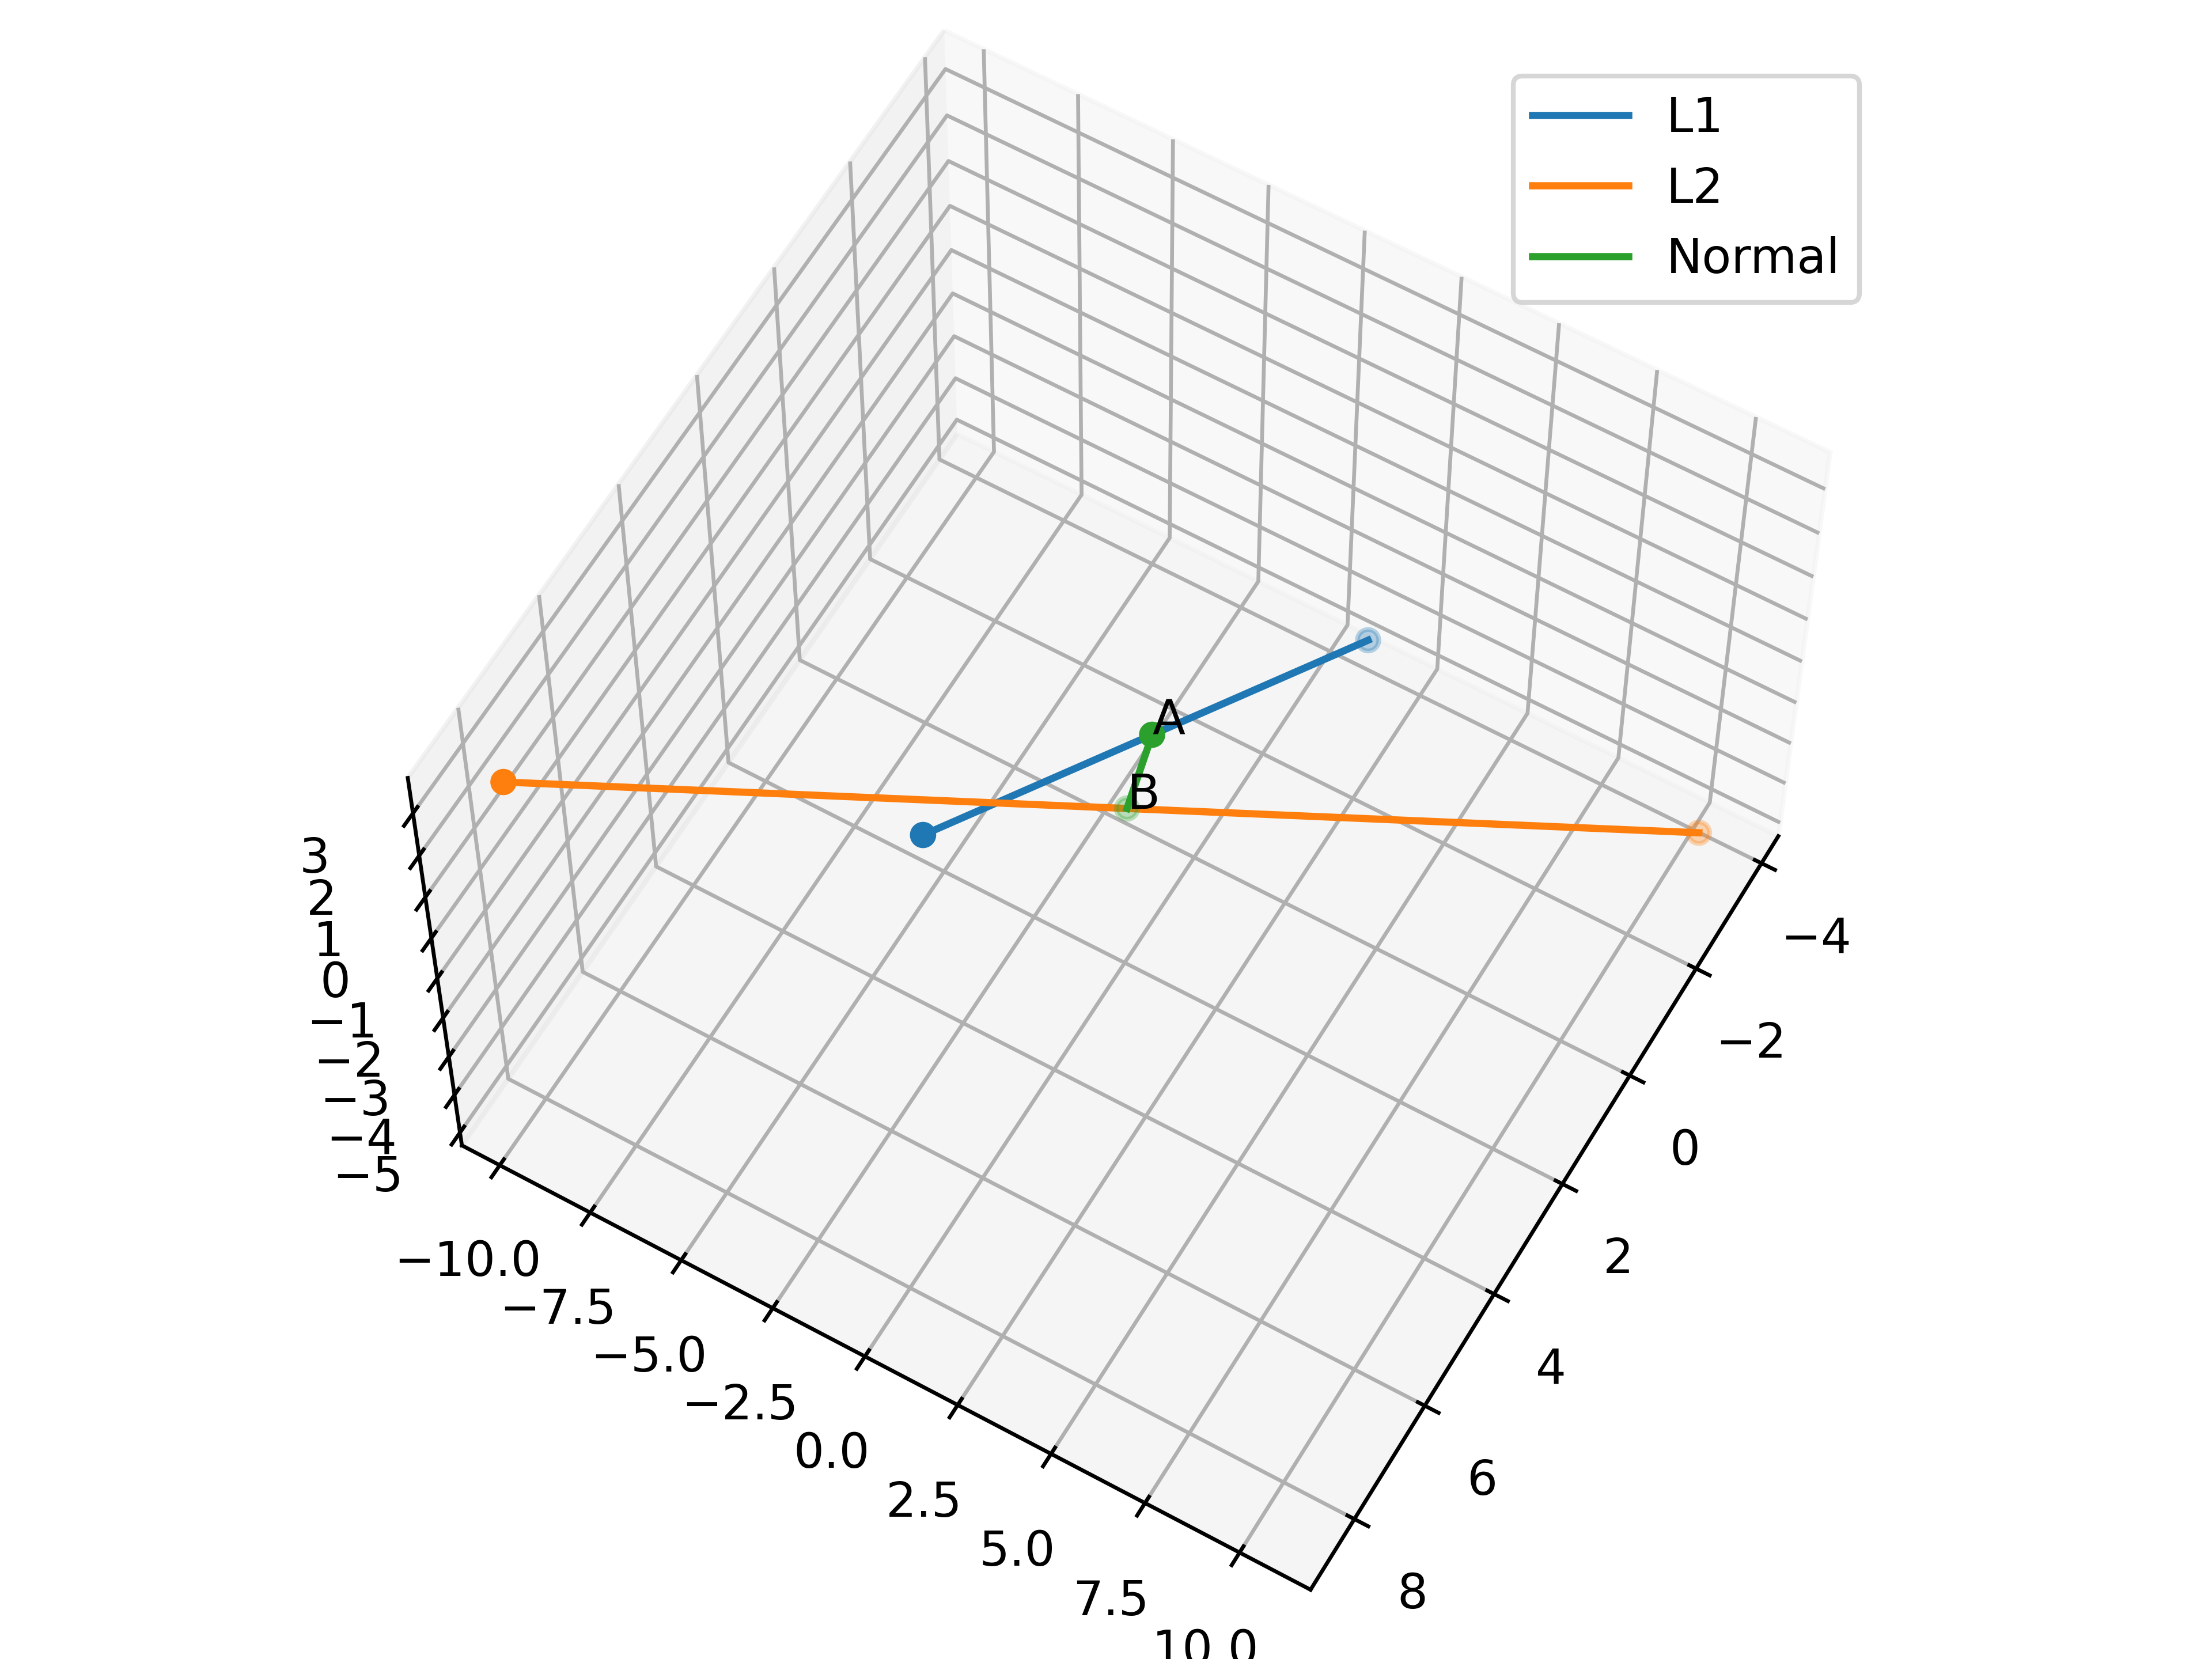
\includegraphics[width=\columnwidth]{./chapters/12/11/2/e11/svd/figs/skew.png}
\caption{$AB$ is the required shortest distance.}
	\label{fig:chapters/12/11/2/e11/svd/}
\end{figure}
\end{enumerate} 

\item Find the shortest distance between the lines given by $\overrightarrow{r}=(8+3\lambda\hat{i}-(9+16\lambda)\hat{j}+(10+7\lambda)\hat{k}$ and $\overrightarrow{r}=15\hat{i}+29\hat{j}+5\hat{k}+\mu(3\hat{i}+8\hat{j}-5\hat{k}).$
\end{enumerate}

%
\section{Optimization}
\subsection{Introduction}
\renewcommand{\theequation}{\theenumi}
\begin{enumerate}[label=\thesubsection.\arabic*.,ref=\thesubsection.\theenumi]
\numberwithin{equation}{enumi}
%
%
\item Express the problem of finding the distance of the point $\vec{P}=\myvec{3\\-5}$ from the line 
\label{prob:opt_line_dist}
\begin{align}
\label{eq:opt_line_nor}
L: \quad \myvec{3 & – 4}\vec{x}  = 26
\end{align}
%
as an optimization problem.
\\
\solution The given problem can be expressed as
%
\begin{align}
\label{eq:opt_line_dist}
\min_{\vec{x}}g(\vec{x}) &= \norm{\vec{x}-\vec{P}}^2
\\
\text{s.t.} \quad \vec{n}^T\vec{x} &= c
\label{eq:opt_line_dist_nor}
\end{align}
%
where 
%
\begin{align}
\vec{n} &= \myvec{3\\-4}
\\
c&=26
\end{align}
%
\item Explain Problem \ref{prob:opt_line_dist} through a plot and find a graphical solution.
%
\item Solve \eqref{eq:opt_line_dist} using cvxpy.
%
\\
\solution  The following code yields
%	
\begin{lstlisting}
codes/opt/line_dist_cvx.py
\end{lstlisting}
%
\begin{align}
\vec{x}_{\min} &= \myvec{2.64\\-4.52},
\\
g\brak{\vec{x}_{\min}} &= 0.6
\end{align}
%

\item Convert  \eqref{eq:opt_line_dist} to an {\em unconstrained} optimization problem.
%
\\
%
\solution $L$ in \eqref{eq:opt_line_nor} can be expressed in terms of the direction vector $\vec{m}$ as
\begin{align}
\label{eq:opt_line_dir}
\vec{x} = \vec{A} + \lambda \vec{m}, 
\end{align}
where $\vec{A}$ is any point on the line and 
%
\begin{align}
\label{eq:opt_line_orth}
\vec{m}^T\vec{n} = 0
\end{align}
%
Substituting \eqref{eq:opt_line_dir} in \eqref{eq:opt_line_dist}, an unconstrained optimization problem 
\begin{align}
\label{eq:opt_line_dist_uncon}
\min_{\lambda}f(\lambda) = \norm{\vec{A} + \lambda \vec{m}-\vec{P}}^2 
\end{align}
%
is obtained.
%
\item Solve \eqref{eq:opt_line_dist_uncon}.
%
\\
\solution 
\begin{align}
f(\lambda) 
& = \brak{ \lambda \vec{m}+\vec{A} -\vec{P}}^T \brak{ \lambda \vec{m}+\vec{A} -\vec{P}}
\\
&= \lambda^2 \norm{\vec{m}}^2 +2\lambda \vec{m}^T\brak{\vec{A} -\vec{P}} 
\nonumber \\
&\quad + \norm{\vec{A} -\vec{P}}^2
\label{eq:opt_line_dist_uncon_dist}
\end{align}
\begin{align}
\because f^{(2)}\lambda = 2\norm{\vec{m}}^2 > 0
\end{align}
%
the minimum value of $f(\lambda)$ is obtained when 
%
\begin{align}
 f^{(1)}(\lambda) &= 2\lambda\norm{\vec{m}}^2 + 2 \vec{m}^T\brak{\vec{A} -\vec{P}} =0
\\
\implies \lambda_{\min} &= -\frac{\vec{m}^T\brak{\vec{A} -\vec{P}}}{\norm{\vec{m}}^2}
\label{eq:opt_line_dist_uncon_lam_min}
\end{align}
%
Choosing $\vec{A}$ such that 
%
\begin{align}
\vec{m}^T\brak{\vec{A} -\vec{P}} &= 0,
\label{eq:opt_line_dist_uncon_trick}
\end{align}
%
substituting in \eqref{eq:opt_line_dist_uncon_lam_min},
%
\begin{align}
\label{eq:opt_line_dist_uncon_lam0}
\lambda_{\min} &= 0 \quad \text{and}
\\
\vec{A} -\vec{P} &= \mu \vec{n}
\label{eq:opt_line_dist_uncon_mu}
\end{align}
for some constant $\mu$. \eqref{eq:opt_line_dist_uncon_mu}
 is a consequence of \eqref{eq:opt_line_orth} and \eqref{eq:opt_line_dist_uncon_trick}. Also, from 
\eqref{eq:opt_line_dist_uncon_mu},
%
\begin{align}
\vec{n}^T\brak{\vec{A} -\vec{P} } &= \mu \norm{\vec{n}}^2
\\
\implies \mu & = \frac{\vec{n}^T\vec{A} -\vec{n}^T\vec{P} }{\norm{\vec{n}}^2} = \frac{c -\vec{n}^T\vec{P} }{\norm{\vec{n}}^2}
\label{eq:opt_line_dist_uncon_mu_sol}
\end{align}
%
from \eqref{eq:opt_line_dist_nor}.
%, where $\mu$ is some constant.
Substituting $\lambda_{\min} = 0$ in \eqref{eq:opt_line_dist_uncon},
%\label
%Thus, the shortest distance from $\vec{P}$ to $L$ is
%
\begin{align}
\min_{\lambda}f(\lambda) =  \norm{\vec{A} -\vec{P}}^2 = \mu^2\norm{\vec{n}}^2
\label{eq:opt_line_dist_uncon_f}
\end{align}
upon substituting from \eqref{eq:opt_line_dist_uncon_mu}. The distance between $\vec{P}$ and ${L}$ is then obtained from \eqref{eq:opt_line_dist_uncon_f} as
% obtained as 
\begin{align}
\norm{\vec{A} -\vec{P}} &= \abs{\mu}\norm{\vec{n}}
\\
&= \frac{\abs{\vec{n}^T\vec{P} -c }}{\norm{\vec{n}}}
\label{eq:opt_line_dist_uncon_f_closed}
\end{align}
after substituting for $\mu$ from  \eqref{eq:opt_line_dist_uncon_mu_sol}. Using the corresponding values from Problem \eqref{prob:opt_line_dist} in \eqref{eq:opt_line_dist_uncon_f_closed},
%
\begin{align}
\min_{\lambda}f(\lambda) =  0.6
\end{align}

%
%
\end{enumerate}

\subsection{Convex Function}
\renewcommand{\theequation}{\theenumi}
%\subsection{Problem}

\begin{enumerate}[label=\thesubsection.\arabic*.,ref=\thesubsection.\theenumi]
\numberwithin{equation}{enumi}

\item
The following python script plots 
%
\begin{align}
f(\lambda) = a\lambda^2 + b\lambda + d
\label{eq:opt_parab}
\end{align}
%
for 
\begin{align}
a &= \norm{\vec{m}}^2 > 0
\\
b &= \vec{m}^T\brak{\vec{A} -\vec{P}} 
\\
c &= \norm{\vec{A} -\vec{P}}^2
\end{align}
where $\vec{A}$ is the intercept of the line $L$ in \eqref{eq:opt_line_nor}
on the x-axis and the points
\begin{align}
\vec{U} &= \myvec{\lambda_1\\f(\lambda_1)}, 
\vec{V} = \myvec{\lambda_2\\f(\lambda_2)}
\\
\vec{X} &= \myvec{t \lambda_1 + \brak{1-t}\lambda_2 \\ f\sbrak{t \lambda_1 + \brak{1-t}\lambda_2}},
\\
\vec{Y} &= \myvec{t \lambda_1 + \brak{1-t}\lambda_2 \\ t f\brak{\lambda_1} + \brak{1-t}f\brak{\lambda_2}}
\end{align}
%
for 
\begin{align}
\lambda_1 = -3, 
\lambda_2 = 4, 
t = 0.3
\end{align}
in Fig. \ref{fig:conv_def}. Geometrically, this means that any point $\vec{Y}$ between the points $\vec{U}, \vec{V}$ on the line $UV$ is always above the point $\vec{X}$ on the curve $f(\lambda)$.
Such a  function $f$ is defined to be {\em convex} function 
%
\begin{lstlisting}
codes/opt/1.2.py
\end{lstlisting}
%
%%
\begin{figure}[!ht]
\centering
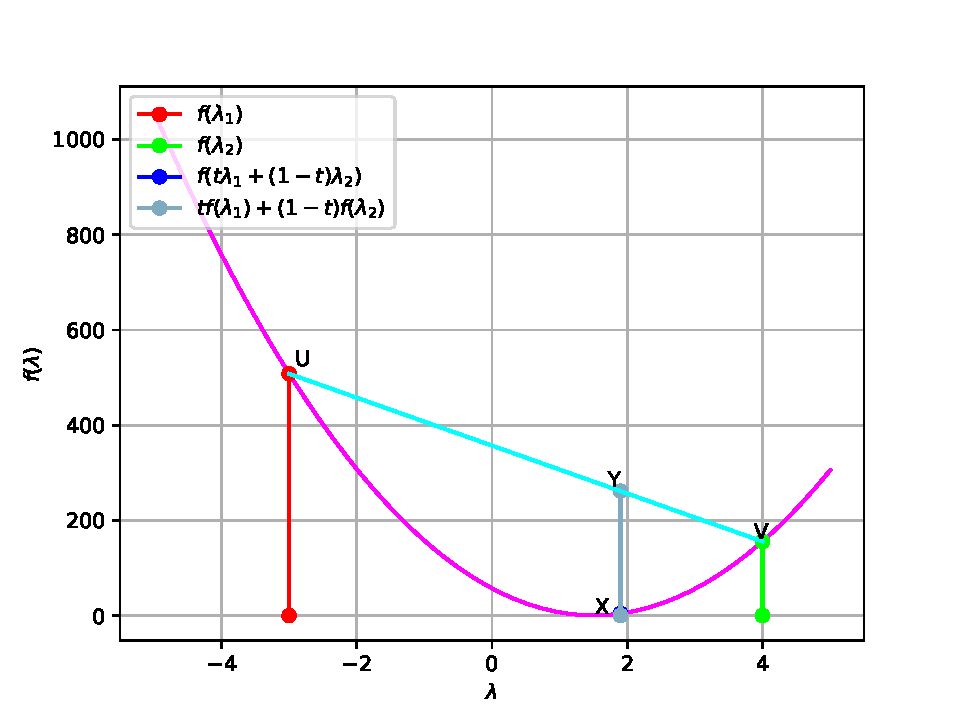
\includegraphics[width=\columnwidth]{./figs/opt/convex.eps}
\caption{ $f(\lambda)$ versus $\lambda$}.
\label{fig:conv_def}	
\end{figure}
%
\item Show that
%
\begin{align}
\label{eq:convex_def}
f\sbrak{t \lambda_1 + \brak{1-t}\lambda_2} \leq 
t f\brak{\lambda_1} + \brak{1-t}f\brak{\lambda_2}
\end{align}
%
for $\quad 0 < t < 1$.  This is true for any convex function.
%
\item Show that 
%
\begin{equation}
\eqref{eq:convex_def} \quad \implies f^{(2)}(\lambda) > 0
\end{equation}
%
\item Show that a covex function has a unique minimum.
%
\end{enumerate}
%

\subsection{Gradient Descent}
\renewcommand{\theequation}{\theenumi}
\begin{enumerate}[label=\thesubsection.\arabic*.,ref=\thesubsection.\theenumi]
\numberwithin{equation}{enumi}
%\item Consider the problem of finding the square root of a number $c$.  This can be expressed as the equation
%%
%\begin{equation}
%\label{eq:root}
%x^2 -c= 0
%\end{equation}
%%
%
%\item
%Sketch the function for different values of $c$
%%
%\begin{equation}
%f(x)= x^{3}-3xc
%\end{equation}
%%
%and comment upon its convexity.
%
%\item
%Show that \eqref{eq:root} results from
%\begin{align}
%\min_{x}f(x)= x^{3}-3xc
%\end{align}

\item
Find a numerical solution for \eqref{eq:parab}

%
%\begin{align}
%f(\lambda) = a\lambda^2 + b\lambda + d
%\end{align}
%
%\eqref{eq:root}.
%\\
\solution
A numerical solution for \eqref{eq:parab} is obtained as
%
\begin{align}
\lambda_{n+1}&=\lambda_{n}-\mu f^{\prime}\brak{\lambda_n}
\\
&=\lambda_{n} -\mu \brak{2a\lambda_n+b}
\label{eq:gradient}
\end{align}

%\begin{align}
%x_{n+1}&=x_{n}-{\frac {f(x_{n})}{f^{\prime}(x_{n})}}
%\\
%&=x_{n} -\frac{x^2_{n}-c}{2x_n} 
%\\
%&=\frac{1}{2}\sbrak{x_{n} +\frac{c}{x_n} }
%\label{eq:newton}
%\end{align}
%
where $\lambda_0$ is an inital guess and $\mu$ is a variable parameter. The choice of these parameters is very important since they decide how fast the algorithm converges.
%
\item
Write a program to implement \eqref{eq:gradient}.
%
\\
\solution Download and execute
\begin{lstlisting}
codes/opt/gd.py
\end{lstlisting}
%
\item Find a closed form solution for $\lambda_n$ in  \eqref{eq:gradient} using the one sided Z transform.
%
\item Find the condition for which \eqref{eq:gradient} converges, i.e.
\begin{align}
\lim_{n \to \infty}\abs{\lambda_{n+1}-\lambda_n} = 0
\end{align}
\end{enumerate}


\subsection{Lagrange Multipliers}
\renewcommand{\theequation}{\theenumi}
\begin{enumerate}[label=\thesubsection.\arabic*.,ref=\thesubsection.\theenumi]
\numberwithin{equation}{enumi}

\item
	\label{convex_code}
Find
\begin{align}
\label{eq:opt_line_nor_h}
	\min_{\mbf{x}}g\brak{\mbf{x}} = \norm{\vec{x}-\vec{P}}^2 = r^2 \\
\text{s.t.} \quad 	h\brak{\mbf{x}} = \vec{n}^T\vec{x} - c = 0\label{eq2_1_line}
%	\quad g\brak{\mbf{x}} = x_1 + x_2 - 9 = 0
\end{align}
by plotting the circles $g\brak{\vec{x}}$
%
%\begin{equation}
% \norm{\vec{x}-\myvec{8\\6}}^2 =r^2
%%(x_1-8)^2 + (x_2-6)^2 = r^2
%\end{equation}
%
% $\mbf{x}= \myvec{x_1\\x_2}$, 
for different values of $r$ along with the line $g\brak{\mbf{x}}$.
%
%\begin{equation}
%\label{eq2_1_line}
%g\brak{\mbf{x}} = \myvec{1 & 1}\vec{x} - 9 = 0
%\end{equation} 
%
\\
\solution 
The following code plots Fig. \ref{fig:concirc}	

%	
\begin{lstlisting}
codes/opt/concirc.py
\end{lstlisting}

%
\begin{figure}[!ht]
\centering
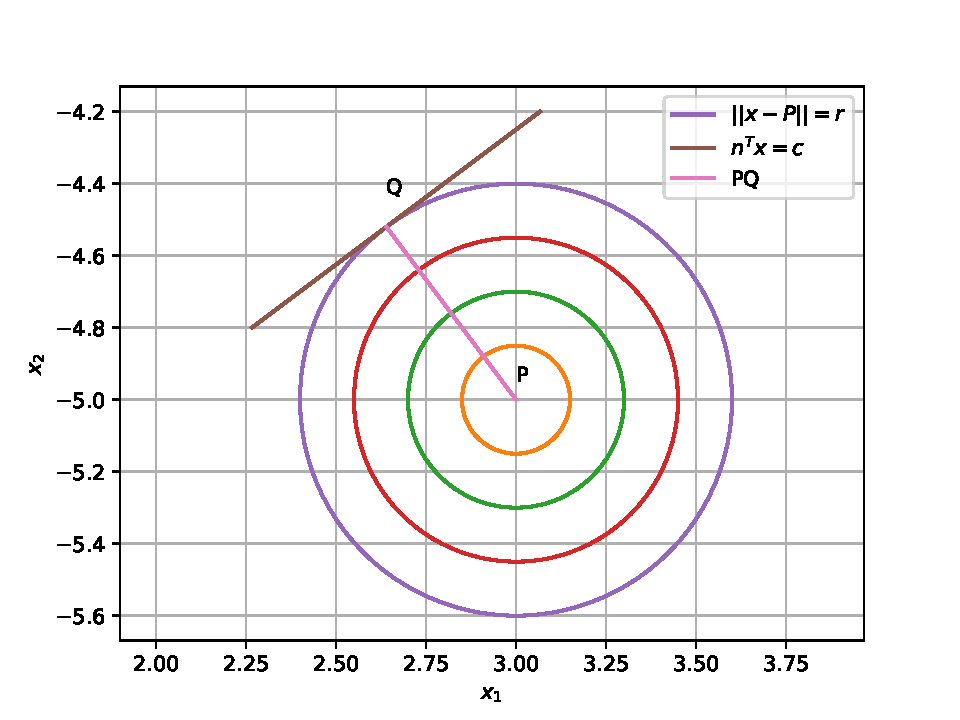
\includegraphics[width=\columnwidth]{./figs/opt/concirc.eps}
\caption{ Finding $ \displaystyle \min_{\mbf{x}}g\brak{\mbf{x}}$}.
\label{fig:concirc}	
\end{figure}
%
\item By solving the quadratic equation obtained from \eqref{eq:opt_line_nor_h},
show that 
\label{prob:minr}
\begin{align}
\min_{\vec{x}} r = \frac{3}{5}, \vec{x}_{\min} = \vec{Q}  = \myvec{2.64\\-4.52}
\end{align}
%
%and find $,
%$ that minimizes $r$. By labeling  $\vec{Q}$ 
In Fig. \ref{fig:concirc}, it can be seen  that $\vec{Q}$ is the point of contact of the line $L$ with the circle of minimum radius $r = \frac{3}{5}$.
%Obtain a theoretical solution for problem \ref{convex_code} 
%%using coordinate geometry.
%
%\solution 
%From \eqref{eq2_1_line} and \eqref{eq2_1_circ}, 
%%
%\begin{align}
%r^2 & = (x_1-8)^2 + (3- x_1)^2 \\
%&= 2 x_1^2 - 22 x_1 + 73 \\
%\Rightarrow r^2 &= \frac{\brak{2x_1-11}^2 + 5^2}{2}
%\end{align}
%%
%which is minium when $x_1 = \frac{11}{2}, x_2 = \frac{7}{2}$.  The minimum value is $\frac{25}{2}$ and 
%the radius $r = \frac{5}{\sqrt{2}}$.
\item Show that 
\begin{align}
\label{eq:lagrange_n}
\nabla h(\vec{x}) =  \myvec{3 \\ -4} = \vec{n}
\end{align}
where
\begin{equation}
\nabla =  
\begin{pmatrix}
\frac{\partial}{\partial x_1} \\
\frac{\partial}{\partial x_2} 
\end{pmatrix}
\end{equation}

\item Show that 
\begin{align}
\nabla g(\vec{x}) = 2\cbrak{\vec{x}-\myvec{3 \\ -5}} = 2\cbrak{\vec{x}-\vec{P}}
\label{eq:lagrange_pq}
\end{align}
%
%is the direction vector of the normal at $\vec{x}$.
\item From Fig. \ref{fig:concirc}, show that 
\begin{align}
\label{eq:opt_normal}
\nabla g(\vec{Q}) = \lambda \nabla h(\vec{Q}),
\end{align}
%
\solution In Fig. \ref{fig:concirc}, PQ is the normal to the line $L$, represented by $h\brak{\vec{x}}$. 
$\because$ the normal vector of $L$ is in the same direction as $PQ$,  for some constant $k$, 
%
\begin{align}
%\label{eq:opt_normal}
\brak{\vec{Q}-\vec{P}} = k \vec{n}
\end{align}
%
which is the same as \eqref{eq:opt_normal} after substituting from \eqref{eq:lagrange_n}.
 and \eqref{eq:lagrange_pq}.
%where $\vec{p}$ is the point of contact.
\item Use \eqref{eq:opt_normal} and $\vec{h(\vec{Q})}=0$ from \eqref{eq2_1_line} to obtain $\vec{Q}$.
\\
\solution From the given equations, we obtain
\begin{align}
\brak{\vec{Q}-\vec{P}}-\lambda \vec{n} &= 0 
\\
\vec{n}^T\vec{Q} - c &= 0
\label{eq:lagrange_mat_eq}
\end{align}
%
which can be simplifed to obtain
%
\begin{align}
\myvec{\vec{I} & -\vec{n} \\ \vec{n}^T & 0}\myvec{\vec{Q}\\ \lambda} = \myvec{\vec{P}\\c}
%\vec{Q} = \vec{P}+\frac{\brak{c-\vec{n}^T\vec{P}}}{\norm{\vec{n}}^2}\vec{n}
\label{eq:lagrange_mat_sol}
\end{align}
The following code computes the solution to \eqref{eq:lagrange_mat_sol}
%
\begin{lstlisting}
codes/opt/lagmul.py
\end{lstlisting}

\item
\label{lagrange}
	Define 
	\begin{equation}
	\label{lagrangian}
	C\brak{\mbf{x},\lambda} = g\brak{\mbf{x}} - \lambda h\brak{\mbf{x}}%, \quad \lambda > 0
	\end{equation}
and show that $\vec{Q}$ can also be obtained by 
solving the equations
%
\begin{align}
\nabla C\brak{\mbf{x},\lambda} &= 0.
\label{tangent}
\end{align}
%
What is the sign of $\lambda$?  $C$ is known as the Lagrangian and the above technique is known as the Method of Lagrange Multipliers.

%\solution
%From \eqref{eq2_1_line} and \eqref{eq2_1_circ}, 
%%
%\begin{align}
%L\brak{\mbf{x},\lambda} &= (x_1-8)^2 + (x_2-6)^2 - \lambda \brak{x_1 + x_2 - 9} \\
%\Rightarrow \nabla L\brak{\mbf{x},\lambda}  & = 
%\begin{pmatrix}
%2x_1  - 16 - \lambda \\
%2x_2 - 12 - \lambda \\
%x_1 + x_2 -9
%\end{pmatrix}
%\\
%&=
%\begin{pmatrix}
%2 &0 & - 1 \\
%0 &2 & - 1 \\
%1 & 1 & 0 
%\end{pmatrix}
%\begin{pmatrix}
%x_1 \\
%x_2 \\
%\lambda
%\end{pmatrix}
%= 
%\begin{pmatrix}
%16 \\
% 12 \\
%9
%\end{pmatrix}
%=
%0 
%\\
%\Rightarrow 
%\begin{pmatrix}
%x_1 \\
%x_2 \\
%\lambda
%\end{pmatrix}
%&= 
%\begin{pmatrix}
%\frac{11}{2} \\
% \frac{7}{2} \\
%-5
%\end{pmatrix}
%\end{align}
%%
%using the following python script.  Note that this method yields the same result as the previous exercises.  Thus, $\lambda$ is negative.
%	
\item Obtain $\vec{Q}$ using gradient descent.
\\
\solution
\begin{lstlisting}
codes/opt/gd_lagrange.py
\end{lstlisting}

\end{enumerate}

\subsection{Quadratic Programming}
\renewcommand{\theequation}{\theenumi}
\begin{enumerate}[label=\thesubsection.\arabic*.,ref=\thesubsection.\theenumi]
\numberwithin{equation}{enumi}

\item An apache helicopter of the enemy is flying along the curve given by 
	\label{prob:dist_pt_parab}
\begin{align}
\label{eq:dist_pt_parab}
y = x^2 +7
\end{align}
%
A soldier, placed at 
\begin{align}
\vec{P} = \myvec{3\\7}.  
\end{align}
%
wants to shoot the heicopter when it is nearest to him.  Express this as an optimization problem.
%\item
%Express the problem of 
%finding the point on the curve 
%\begin{align}
%\label{eq:dist_pt_parab}
%x^2 = 2y
%\end{align}
%%
%nearest to the point 
%\begin{align}
%\vec{P} = \myvec{0\\5}.  
%\end{align}
%%
%as an optiimization problem.
\\
\solution The given problem can be expressed as
\begin{align}
\label{eq:qp_dist_pt_parab}
\min_{\vec{x}}\norm{\vec{x}-\vec{P}}^2
\\
\text{s.t. }\vec{x}^T\vec{V}\vec{x} + \vec{u}^T\vec{x}  +d = 0
\end{align}
%
where
%
\begin{align}
\vec{V} &= \myvec{1 & 0\\0 & 0}
\\
\vec{u} &= -\myvec{0 \\ 1}
\\
d &= 7
\end{align}
\item Show that the constraint in \ref{eq:qp_dist_pt_parab} is nonconvex.
\item Show that the following {\em relaxation} makes \eqref{eq:qp_dist_pt_parab} a convex optimization problem.
%
\begin{align}
\label{eq:qp_dist_pt_parab_conv}
\min_{\vec{x}}\brak{\vec{x}-\vec{P}}^T\brak{\vec{x}-\vec{P}}
\\
\text{s.t. }\vec{x}^T\vec{V}\vec{x} + \vec{u}^T\vec{x}  \le 0
\end{align}
%
%
\item Solve \eqref{eq:qp_dist_pt_parab_conv} using cvxpy.
\\
\solution  The following code yields the minimum distance as 2.236 and the nearest point on the curve as
%
\begin{align}
\vec{Q} &= \myvec{1\\8}
\end{align}

\begin{lstlisting}
codes/opt/qp_cvx.py
\end{lstlisting}

\item Solve \eqref{eq:qp_dist_pt_parab_conv} using the method of Lagrange multipliers.
\item Graphically verify the solution to Problem \ref{prob:dist_pt_parab}. 
%by drawing a figure.
\\
\solution 
The following code plots Fig. \ref{fig:qp_parab}
%	
\begin{lstlisting}
codes/opt/qp_parab.py
\end{lstlisting}

%
\begin{figure}[!ht]
\centering
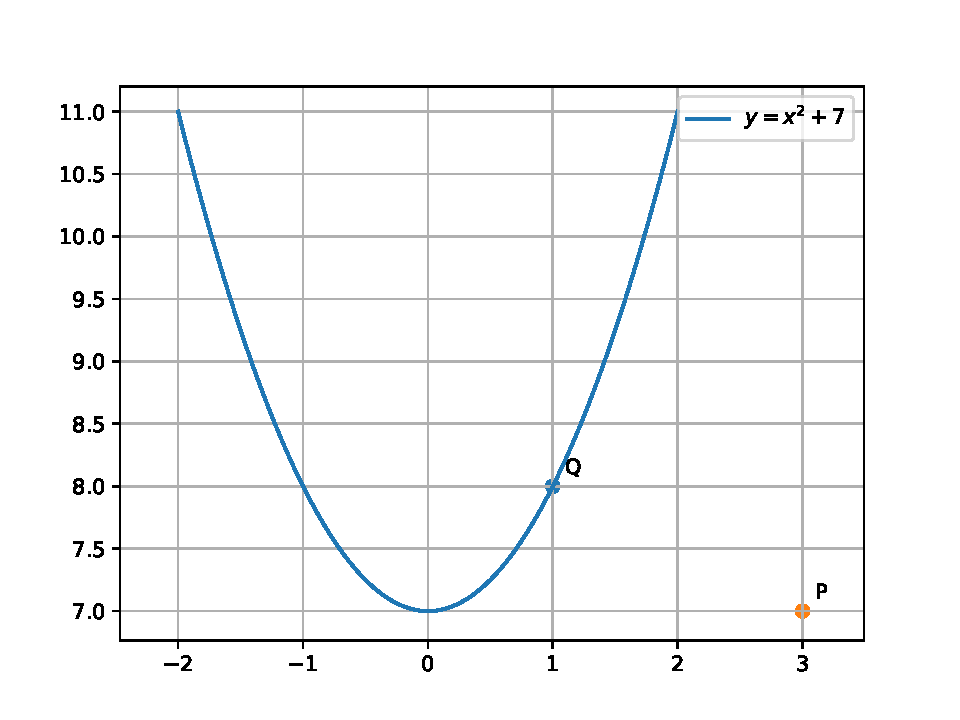
\includegraphics[width=\columnwidth]{./figs/opt/qp_parab.eps}
\caption{ $\vec{Q}$ is closest to $\vec{P}$}.
\label{fig:qp_parab}
\end{figure}
%
%\item Frame 	
% as an optimization problem.
%\label{prob:qp_dist_pt_parab}
%\\
%
%\solution 
%From \eqref{eq2_1_line} and \eqref{eq2_1_circ}, 
%%
%\begin{align}
%r^2 & = (x_1-8)^2 + (3- x_1)^2 \\
%&= 2 x_1^2 - 22 x_1 + 73 \\
%\Rightarrow r^2 &= \frac{\brak{2x_1-11}^2 + 5^2}{2}
%\end{align}
%%
%which is minium when $x_1 = \frac{11}{2}, x_2 = \frac{7}{2}$.  The minimum value is $\frac{25}{2}$ and 
%the radius $r = \frac{5}{\sqrt{2}}$.
%	
%\begin{lstlisting}
%codes/opt/optimization/lagmul.py
%\end{lstlisting}
\item Solve \eqref{eq:qp_dist_pt_parab_conv} using gradient descent.
%
\end{enumerate}

\subsection{Semi Definite Programming}
\renewcommand{\theequation}{\theenumi}
\begin{enumerate}[label=\thesubsection.\arabic*.,ref=\thesubsection.\theenumi]
\numberwithin{equation}{enumi}

%\item An apache helicopter of the enemy is flying along the curve given by 
%	\label{prob:dist_pt_parab_sdp}
%\begin{align}
%\label{eq:dist_pt_parab_sdp}
%y = x^2 +7
%\end{align}
%%
%A soldier, placed at 
%\begin{align}
%\vec{P} = \myvec{3\\7}.  
%\end{align}
%%
%wants to shoot the heicopter when it is nearest to him.  Express this as an optimization problem.
\item
	\label{prob:dist_pt_parab_sdp}
Express the problem of 
finding the point on the curve 
\begin{align}
\label{eq:dist_pt_parab_sdp}
x^2 = 2y
\end{align}
%
nearest to the point 
\begin{align}
\vec{P} = \myvec{0\\5}.  
\end{align}
%
as an optimization problem.
\\
\solution The given problem can be expressed as
%
\begin{align}
\label{eq:qp_dist_pt_parab_sdp_qp}
\min_{\vec{x}}\vec{x}^T\vec{Q}_0\vec{x}+\vec{q}_0^T\vec{x}+c_0
\\
\text{s.t. }\vec{x}^T\vec{Q}_1\vec{x} + \vec{q}_1^T\vec{x} +c_1 \le 0
\end{align}
%
%where $\vec{V} \succeq 0$.
%\begin{align}
%\label{eq:qp_dist_pt_parab_sdp}
%\begin{split}
%\min_{\vec{x}}\vec{X}^T\myvec{\vec{I} & \vec{0} \\ \vec{0} & \vec{0}}\vec{X}-2\myvec{\vec{P}^T & \vec{0}}\vec{X}+\norm{\vec{P}}^2
%\\
%\text{s.t. }\vec{x}^T\vec{V}\vec{x} + \vec{u}^T\vec{x}  = 0
%\end{split}
%\end{align}
%
where
%
\begin{align}
\vec{Q}_0 &= \vec{I}, \vec{Q}_1 = \myvec{1 & 0\\0 & 0}
\\
\vec{q}_0 &=-2\vec{P}, \vec{q}_1 = -2\myvec{0 \\ 1}
\\
c_0 &= \norm{\vec{P}}^2, c_1 = 0
\end{align}
%\item Show that the constraint in 	
%%\label{prob:dist_pt_parab_sdp}
%\eqref{eq:qp_dist_pt_parab_sdp} is nonconvex.
%
\item Show that \eqref{eq:qp_dist_pt_parab_sdp_qp} is equivalent to
\begin{align}
\label{eq:qp_dist_pt_parab_sdp_conv}
\begin{split}
\min_{\vec{x},\theta}\theta
\\
\text{s.t. } \myvec{\vec{I} & \vec{M}_0\vec{x} \\ \vec{x}^T\vec{M}_0^T & -c_0-q_0^T\vec{x}+\theta} &\succeq 0
\\
\myvec{\vec{I} & \vec{M}_1\vec{x} \\ \vec{x}^T\vec{M}_1^T & -c_1-q_1^T\vec{x}} &\succeq 0
\end{split}
\end{align}
%
%\item Show that the following {\em relaxation} makes \eqref{eq:qp_dist_pt_parab_sdp} a convex optimization problem.
%%
%\begin{align}
%\label{eq:qp_dist_pt_parab_sdp_conv}
%\min_{\vec{x}}\brak{\vec{x}-\vec{P}}^T\brak{\vec{x}-\vec{P}}
%\\
%\text{s.t. }\vec{x}^T\vec{V}\vec{x} + \vec{u}^T\vec{x}  \le 0
%\end{align}
%
where
\begin{align}
\vec{Q}_i = \vec{M}_i^T\vec{M}_i, i = 0, 1
\end{align}
%
\item Solve \eqref{eq:qp_dist_pt_parab_sdp_conv} using cvxpy.
\item Graphically verify the solution to Problem \ref{prob:dist_pt_parab_sdp}. 
%\\
%\solution  The following code yields the minimum distance as 2.236 and the nearest point on the curve as
%%
%\begin{align}
%\vec{Q} &= \myvec{1\\8}
%\end{align}
%
%\begin{lstlisting}
%codes/opt/qp_cvx.py
%\end{lstlisting}

\item Solve \eqref{eq:qp_dist_pt_parab_sdp_qp} using the method of Lagrange multipliers.
%by drawing a figure.
%\\
%\solution 
%The following code plots Fig. \label{fig:qp_parab_sdp}
%%	
%\begin{lstlisting}
%codes/opt/qp_parab.py
%\end{lstlisting}
%
%%
%\begin{figure}[!ht]
%\centering
%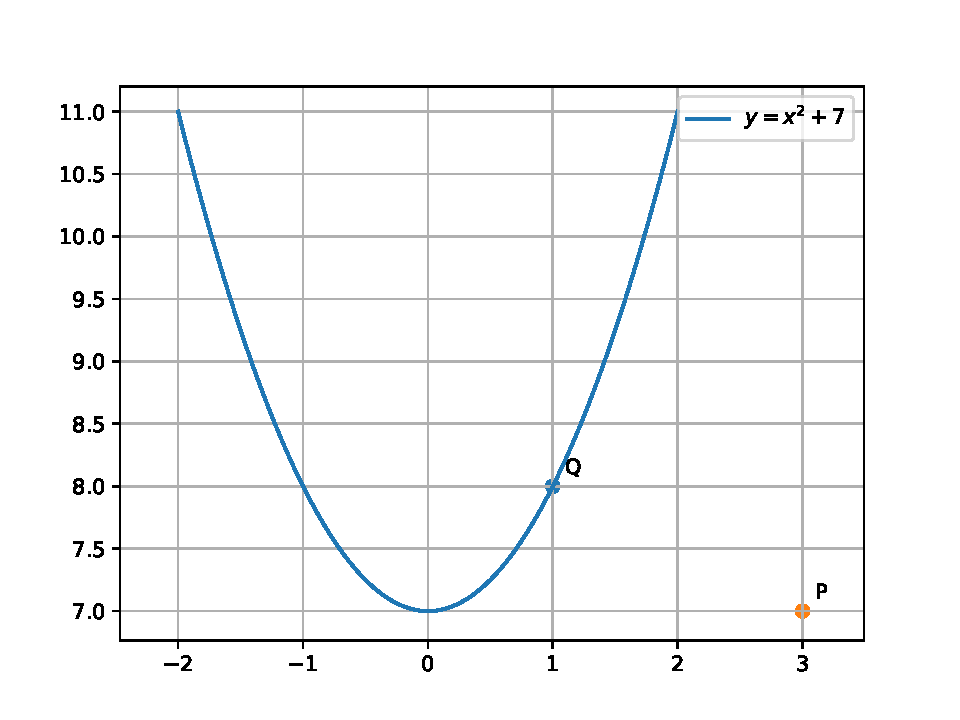
\includegraphics[width=\columnwidth]{./figs/opt/qp_parab.eps}
%\caption{ $\vec{Q}$ is closest to $\vec{P}$}.
%\label{fig:qp_parab_sdp}
%\end{figure}
%
%\item Frame 	
% as an optimization problem.
%\label{prob:qp_dist_pt_parab}
%\\
%
%\solution 
%From \eqref{eq2_1_line} and \eqref{eq2_1_circ}, 
%%
%\begin{align}
%r^2 & = (x_1-8)^2 + (3- x_1)^2 \\
%&= 2 x_1^2 - 22 x_1 + 73 \\
%\Rightarrow r^2 &= \frac{\brak{2x_1-11}^2 + 5^2}{2}
%\end{align}
%%
%which is minium when $x_1 = \frac{11}{2}, x_2 = \frac{7}{2}$.  The minimum value is $\frac{25}{2}$ and 
%the radius $r = \frac{5}{\sqrt{2}}$.
%	
%\begin{lstlisting}
%codes/opt/optimization/lagmul.py
%\end{lstlisting}
%\item Solve \eqref{eq:qp_dist_pt_parab_sdp_conv} using gradient descent.
%
\end{enumerate}

\subsection{Linear Programming}
\renewcommand{\theequation}{\theenumi}
\begin{enumerate}[label=\thesubsection.\arabic*.,ref=\thesubsection.\theenumi]
\numberwithin{equation}{enumi}
%
\item Solve
\label{prob:lp_std}
\begin{align}
\max_{\vec{x}} Z &= \myvec{4 & 1}\vec{x}
\\
s.t. \quad 
\myvec{
1 & 1
\\
3 & 1
}
\vec{x} &\preceq \myvec{50\\90}
\\
\vec{x} &\succeq \vec{0}
\end{align}
%
using cvxpy.
\\
\solution The given problem can be expressed in general as
\begin{align}
\max_{\vec{x}} &\vec{c}^{T}\vec{x}
\\
s.t. \quad \vec{A}\vec{x} &\le \vec{b},
\\
\vec{x} &\succeq\vec{0}
\end{align}
%
where
\begin{align}
\vec{c} &= \myvec{4 \\ 1}
\\
\vec{A} &=
\myvec{
1 & 1
\\
3 & 1
}
\\
\vec{b}&=\myvec{50\\90}
%
\end{align}
%
and can be solved using {\em cvxpy} through the following code
\begin{lstlisting}
codes/opt/lp_cvx.py
\end{lstlisting}
%
to obtain
\begin{align}
\vec{x} = \myvec{30\\0}, Z = 120
\end{align}
%
\item Graphically, show that the {feasible region} in  Problem \ref{prob:lp_std} result in the interior of a convex polygon and the optimal point is one of the vertices.
\solution The following code plots Fig. \ref{fig:lp_feas_reg}.
%
\begin{lstlisting}
codes/opt/lp_cvx.py
\end{lstlisting}
%
\begin{figure}[!ht]
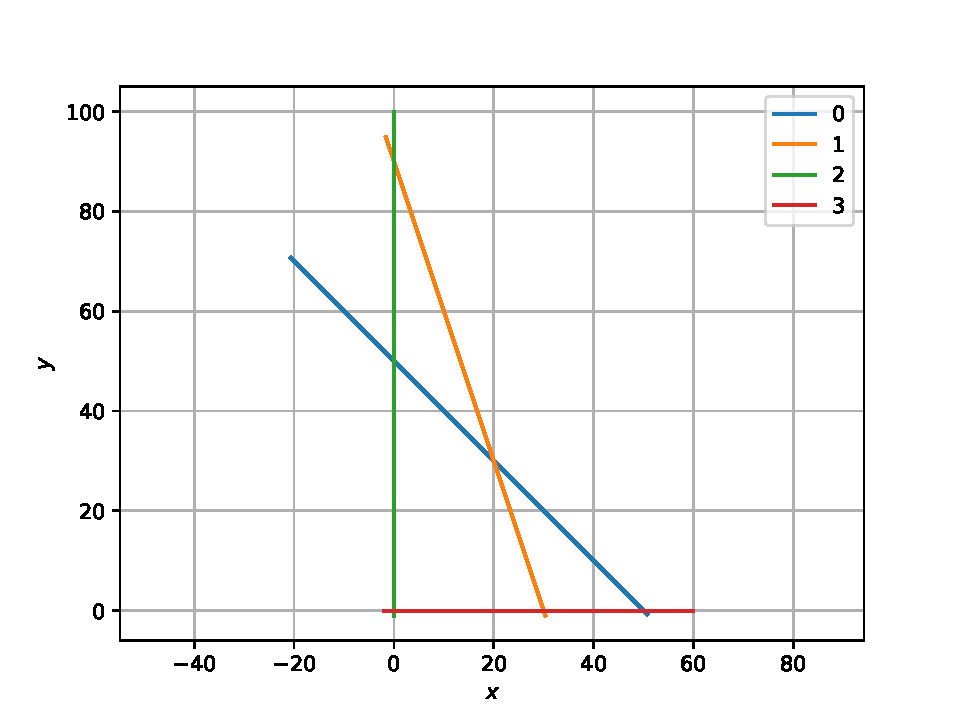
\includegraphics[width=\columnwidth]{./figs/opt/lp_feas_reg.eps}
\caption{}
\label{fig:lp_feas_reg}
\end{figure}

%Verify the solution to graphically.
\item Solve
\begin{align}
\min_{\vec{x}} Z &= \myvec{3 & 9}\vec{x}
\\
s.t. \quad 
\myvec{
1 & 3
\\
-1 & -1
\\
1 & -1
}
\vec{x} &\preceq \myvec{60\\-10\\0}
\\
\vec{x} &\succeq \vec{0}
\label{eq:lp_exam_mult}
\end{align}
\solution The following code
\begin{lstlisting}
codes/opt/lp_cvx_mult.py
\end{lstlisting}
%
is used to obtain
\begin{align}
\vec{x} = \myvec{15\\15}, Z = 180
\end{align}
%
%\item Write a program to plot the constraints for any linear program.

%The region in \eqref{eq:lp_constr} is shown in Fig. \ref{}
\item Solve
\begin{align}
\min_{\vec{x}} Z &= \myvec{-50 & 20}\vec{x}
\\
s.t. \quad 
\myvec{
-2 & 1
\\
-3 & -1
\\
2 & -3
}
\vec{x} &\preceq \myvec{5\\-3\\12}
\\
\vec{x} &\succeq \vec{0}
\end{align}
%
\solution The following code 
\begin{lstlisting}
codes/opt/lp_cvx_nosol.py
\end{lstlisting}
%
shows that the given problem has no solution.
\item Verify all the above solutions using Lagrange multipliers.
\item Repeat the above exercise using the Simplex method.
\item\textbf {(Diet problem)}: A dietician wishes to mix two types of foods in such a
way that vitamin contents of the mixture contain atleast 8 units of vitamin A and 10
units of vitamin C. Food ‘I’ contains 2 units/kg of vitamin A and 1 unit/kg of vitamin C.
Food ‘II’ contains 1 unit/kg of vitamin A and 2 units/kg of vitamin C. It costs
Rs 50 per kg to purchase Food ‘I’ and Rs 70 per kg to purchase Food ‘II’. Formulate
this problem as a linear programming problem to minimise the cost of such a mixture.
\\
\solution Let the mixture contain $x$ kg of food I and $y$ kg of food II.
\\
\begin{table}[!h]
\begin{tabular}{|l|l|l|l|}
\hline
\multirow{2}{*}{Resources} & \multicolumn{2}{l|}{Food} & \multirow{2}{*}{Requirement} \\ \cline{2-3}
                           & I           & II          &                              \\ \hline
Vitamin A                  & 2           & 1           & Atleast 8 Units              \\ \hline
Vitamin C                  & 1           & 2           & Atleast 10 Units             \\ \hline
Cost                       & 50          & 70          &                              \\ \hline
\end{tabular}
\end{table}
%
The given problem can be expressed as
%GOAL: We need to minimize the cost of mixture.\\
%Cost of FOOD I per kg = Rs 50 \\
%Cost of FOOD II per kg = Rs 70 \\
% Minimize $ Z = 50x +70y$\\
% Subject to constraints:\\
% $2x+y>=8$\\
% $x+2y>=10$\\
% $x,y>=0$\\
\begin{align}
\min_{\vec{x}} Z &= \myvec{50 & 70}\vec{x}
\\
s.t. \quad 
\myvec{
2 & 1
\\
1 & 2
%\\
%2 & -3
}
\vec{x} & \succeq \myvec{8\\10}
%\preceq \myvec{5\\-3\\12}
\\
\vec{x} &\succeq \vec{0}
\label{eq:diet}
\end{align}
%
The corner points of the feasible region are available in Table \ref{table:diet_corner_pt} and plotted in Fig. \ref{fig:diet}.
%
\begin{table}[!h]
\begin{tabular}{|l|l|l|l|}
\hline
Corner Point &  $Z=50x+70y$\\
\hline
(0,8)& 560\\
\hline
(2,4)& 380\\
\hline
(10,0)& 500\\
\hline
\end{tabular}
\caption{}
\label{table:diet_corner_pt}
\end{table}
  \begin{figure}[!h]

  \centering
  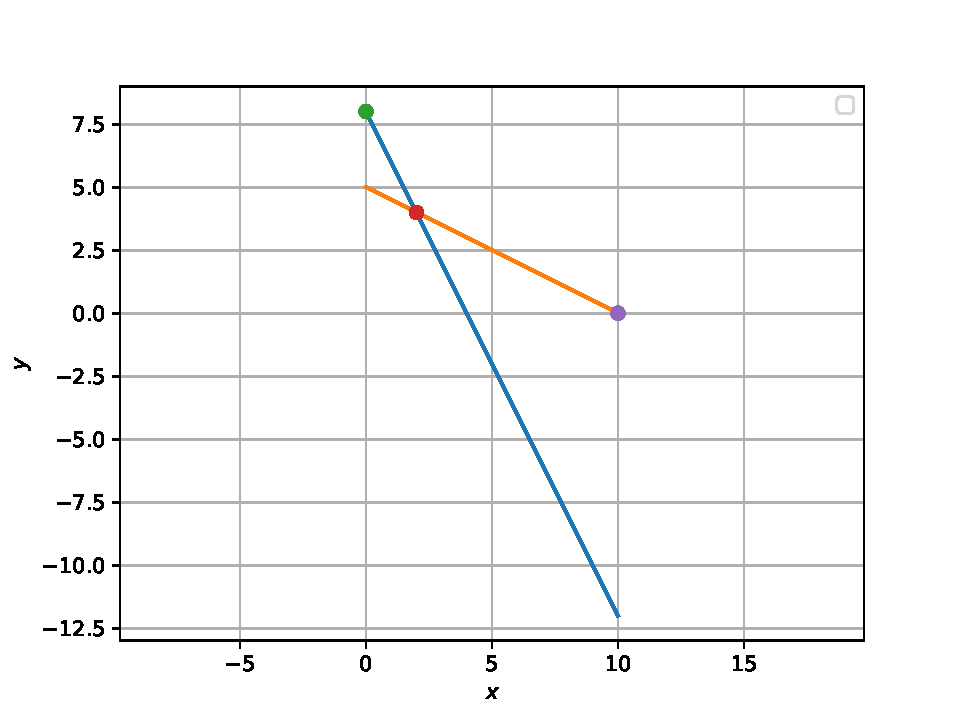
\includegraphics[width=1\linewidth]{./figs/opt/lp_diet.eps}
\caption{}
\label{fig:diet}
  \end{figure}


The smallest value of Z is 380 at the point (2,4). But the feasible region is unbounded therefore we draw the graph of the inequality
\begin{align}
50x +70y<380
\end{align}
to check whether the resulting open half has any point common with the feasible region but on checking it doesn't have any points in common. 
Thus the minimum value of Z is 380 attained at $\myvec{2\\4}$. Hence optimal mixing strategy for the dietician would be to mix 2 Kg of Food I and 4 Kg of Food II.  The following code provides the solution to \eqref{eq:diet}.
%
\begin{lstlisting}
codes/opt/diet.py
\end{lstlisting}



\item \textbf{(Allocation problem)} A cooperative society of farmers has 50 hectare
of land to grow two crops X and Y. The profit from crops X and Y per hectare are
estimated as Rs 10,500 and Rs 9,000 respectively. To control weeds, a liquid herbicide
has to be used for crops X and Y at rates of 20 litres and 10 litres per hectare. Further,
no more than 800 litres of herbicide should be used in order to protect fish and wild life
using a pond which collects drainage from this land. How much land should be allocated
to each crop so as to maximise the total profit of the society?\\
\solution The given problem can be formulated as
\begin{align}
\max_{\vec{x}} Z &= \myvec{10500 & 9000}\vec{x}
\\
s.t. \quad 
\myvec{
20 & 10
}
\vec{x} & \preceq 800
\\
\myvec{
1 & 1
} 
\vec{x} &= 50
\label{eq:allocation}
\end{align}
Fig  \ref{fig:allocation}
shows the intersection of various lines and the optimal point as indicated.
\begin{figure}[h]
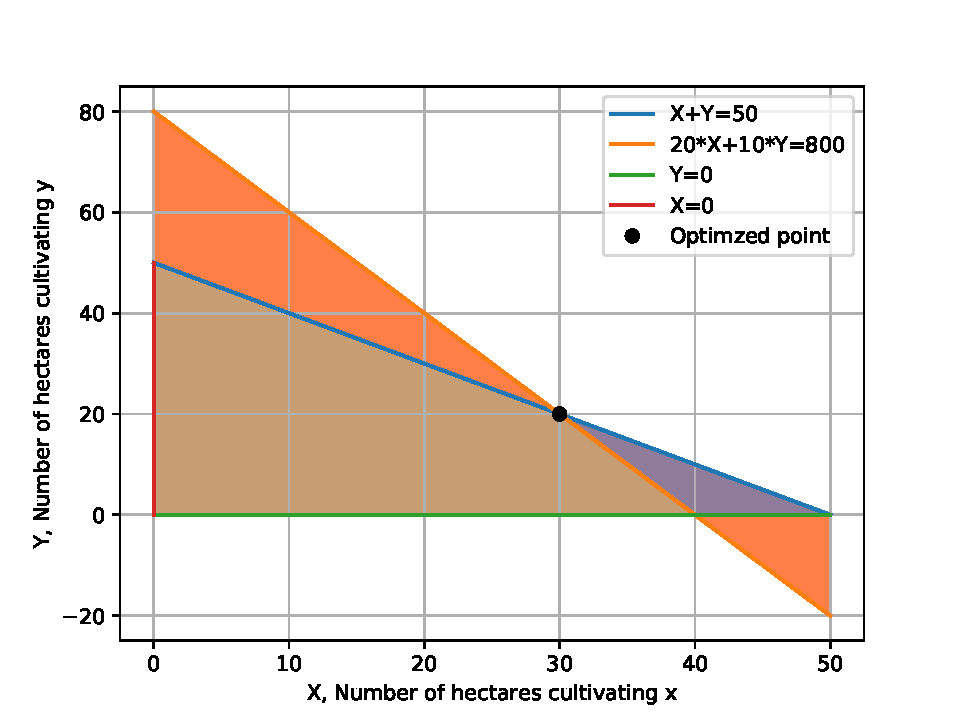
\includegraphics[width=\columnwidth]{./figs/opt/lp_allocation.eps}
\caption{Feasible region for allocation Problem}
\caption{}
\label{fig:allocation}
\end{figure}

The following code provides the solution to \eqref{eq:allocation} at \myvec{30\\20}.
%
\begin{lstlisting}
codes/opt/allocation.py
\end{lstlisting}

\item \textbf{(Manufacturing problem)} A manufacturer has three machines I, II
and III installed in his factory. Machines I and II are capable of being operated for
at most 12 hours whereas machine III must be operated for atleast 5 hours a day. She
produces only two items M and N each requiring the use of all the three machines.
The number of hours required for producing 1 unit of each of M and N on the three
machines are given in the following table:\\

\begin{tabular}{|c|c|c|c|}
\hline
 \multicolumn{3}{|l}{\textbf{ Number of hours required on machines}}& \\ \cline{2-4}
\hline
\textbf {Items}&\textbf{I}&\textbf{II}&\textbf{III}\\
\hline
M&1&2&1\\
\hline
 N&2&1&1.25\\
 \hline 

\end{tabular}

She makes a profit of Rs 600 and Rs 400 on items M and N respectively. How many
of each item should she produce so as to maximise her profit assuming that she can sell
all the items that she produced? What will be the maximum profit?
\\
\solution The given problem can be formulated as
\begin{align}
\max_{\vec{x}} Z &= \myvec{80000&12000}\vec{x}
\\
s.t. \quad 
\myvec{
3 & 4
\\
1 & 3
}
\vec{x} & \preceq \myvec{60\\30}
\label{eq:manufacturing}
\end{align}

Fig  \ref{fig:manufacturing}
shows the intersection of various lines and the optimal point as indicated.
\begin{figure}[h]
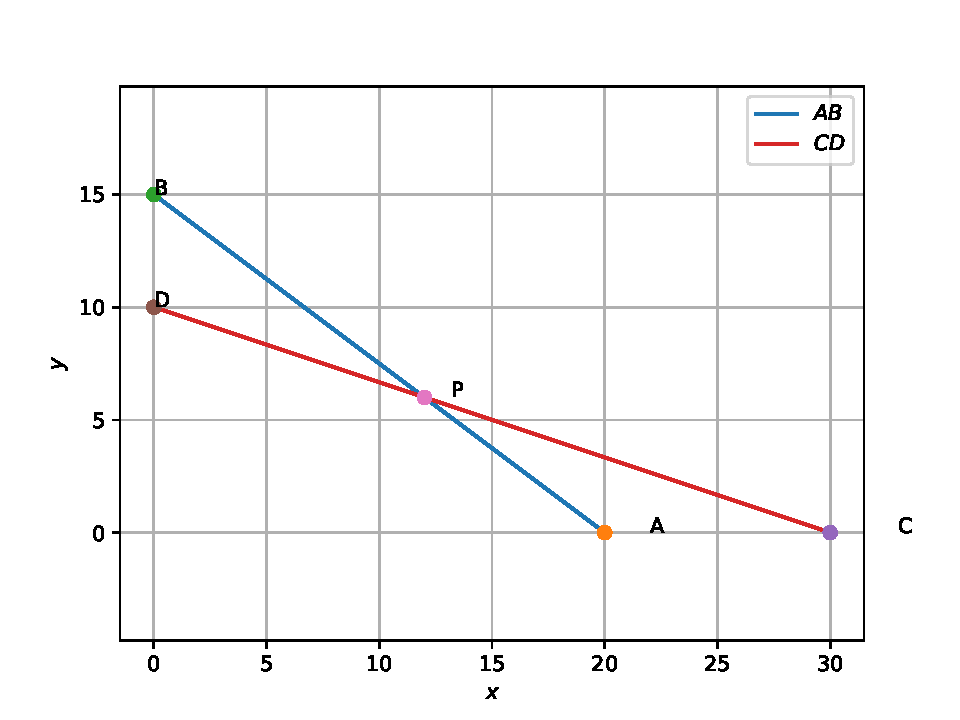
\includegraphics[width=\columnwidth]{./figs/opt/lp_manufacturing.eps}
\caption{Feasible region for manufacturing Problem}
\caption{}
\label{fig:manufacturing}
\end{figure}

The following code provides the solution to \eqref{eq:manufacturing} at \myvec{12\\6}.
%
\begin{lstlisting}
codes/opt/Manufacturing.py
\end{lstlisting}

\item \textbf{(Transportation problem)} There are two factories located one at
place P and the other at place Q. From these locations, a certain commodity is to be
delivered to each of the three depots situated at A, B and C. The weekly requirements
of the depots are respectively 5, 5 and 4 units of the commodity while the production
capacity of the factories at P and Q are respectively 8 and 6 units. The cost of transportation per unit is given below where A,B,C are cost in ruppes:\\
\begin{tabular}{|c|c|c|c|}
\hline
From/To & A & B & C\\
\hline
P & 160 & 100 & 150\\
\hline
Q & 100 &120 & 100\\
\hline
\end{tabular}\\
How many units should be transported from each factory to each depot in order that
the transportation cost is minimum. What will be the minimum transportation cost?
\\
\solution The given problem can be formulated as
\begin{align}
\min_{\vec{x}} Z &= \myvec{10 & -70}\vec{x}
\\
s.t. \quad 
\myvec{
1 & 1
\\
-1 & -1
}
\vec{x} & \preceq \myvec{8\\-4}
\\
\vec{x} &\preceq \myvec{5\\5}
\label{eq:transport}
\end{align}

Fig  \ref{fig:transport}
shows the intersection of various lines and the optimal point indicated as OPT PT.
\begin{figure}[h]
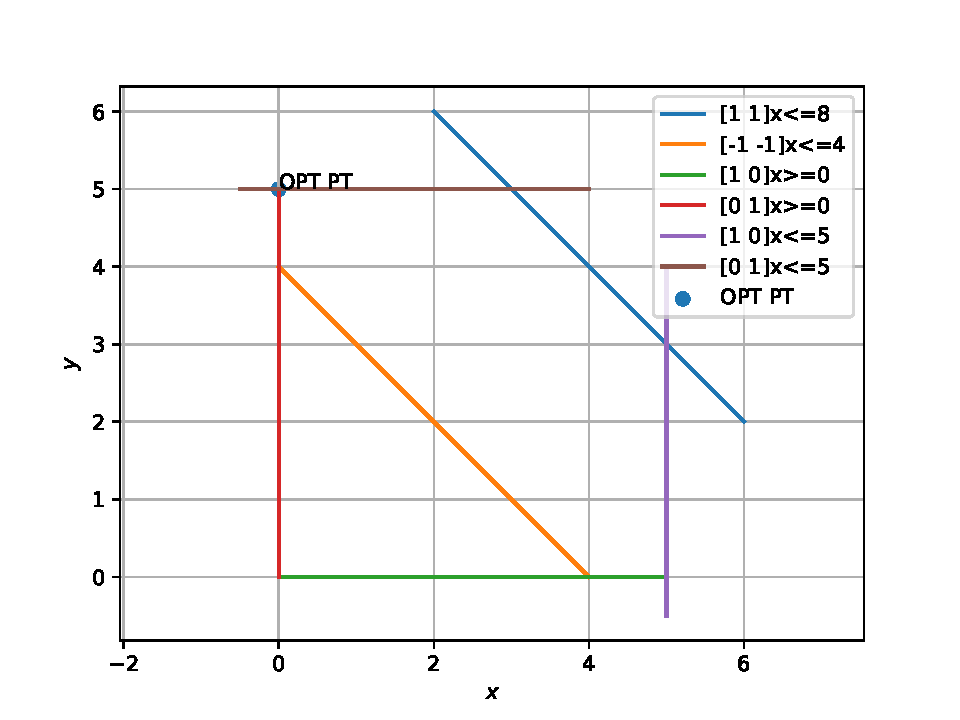
\includegraphics[width=\columnwidth]{./figs/opt/lp_transport.eps}
\caption{Feasible region for Transportation Problem}
\caption{}
\label{fig:transport}
\end{figure}

The following code provides the solution to \eqref{eq:transport} at \myvec{0\\5}.
%
\begin{lstlisting}
codes/opt/Transportation.py
\end{lstlisting}





\end{enumerate}
%    \end{document}
    


\appendices
\section{Proof for the vector form of a conic section}
\label{app:conicdef}
\begin{lemma}
    \label{conics/30/lemma}
    The distance of a point $\vec{P}$ from a line $L: \vec{n}^T\vec{x}=c$ is given by:
    \begin{align}
    d = \frac{\abs{c-\vec{P}^T\vec{n}}}{\norm{\vec{n}}}   
    \end{align}
    \end{lemma}

Using Definition \ref{conics/30/def} and Lemma \ref{conics/30/lemma},  for any point $\vec{x}$ on the conic,
\begin{align}
\norm{\vec{x}-\vec{F}}^2=e^2 \frac{({c-\vec{x}^T\vec{n}})^2}{\norm{\vec{n}}^2}\label{conics/30/eq:1} \\
t(\vec{x}-\vec{F})^T(\vec{x}-\vec{F})=(c-\vec{x}^T\vec{n})^2
\\
t(\vec{x}^T\vec{x}-2\vec{F}^T\vec{x}+\norm{\vec{F}}^2)=c^2+(\vec{x}^T\vec{n})^2-2c\vec{x}^T\vec{n}\\
t\vec{x}^T\vec{x}-(\vec{x}^T\vec{n})^2-2t\vec{F}^T\vec{x}+2c\vec{n}^T\vec{x}=c^2-t\norm{\vec{F}}^2\\
t\vec{x}^T\vec{I}\vec{x}-\vec{x}^T\vec{n}\vec{n}^T\vec{x}+2(c\vec{n}-t\vec{F})^T\vec{x}=c^2-t\norm{\vec{F}}^2\\
\vec{x}^T(t\vec{I}-\vec{n}\vec{n}^T)\vec{x}+2(c\vec{n}-t\vec{F})^T\vec{x}+t\norm{\vec{F}}^2-c^2=0
\end{align}



\section{Proofs for the Parabola}
\label{app:parab}
\renewcommand{\theequation}{\theenumi}
\begin{enumerate}[label=\thesection.\arabic*.,ref=\thesection.\theenumi]
\numberwithin{equation}{enumi}

\item Substituting \eqref{eq:conic_affine} in \eqref{eq:conic_quad_form}
\begin{align}
\brak{\vec{P}\vec{y}+\vec{c}}^T\vec{V}\brak{\vec{P}\vec{y}+\vec{c}}+2\vec{u}^T\brak{\vec{P}\vec{y}+\vec{c}}+ f = 0, 
\end{align}
which can be expressed as
\begin{multline}
\vec{y}^T\vec{P}^T\vec{V}\vec{P}\vec{y}+2\brak{\vec{V}\vec{c}+\vec{u}}^T\vec{P}\vec{y}
\\
+  \vec{c}^T\vec{V}\vec{c} + 2\vec{u}^T\vec{c} + f= 0
\label{eq:conic_simp_one}
\end{multline}
%
From \eqref{eq:conic_simp_one} and \eqref{eq:conic_parmas_eig_def},
\begin{multline}
\vec{y}^T\vec{D}\vec{y}+2\brak{\vec{V}\vec{c}+\vec{u}}^T\vec{P}\vec{y}
\\
+  \vec{c}^T\brak{\vec{V}\vec{c} + \vec{u}}+ \vec{u}^T\vec{c} + f= 0
\label{eq:conic_simp}
\end{multline}
When $\vec{V}^{-1}$ exists,
\begin{align}
%\begin{split}
\vec{V}\vec{c}+\vec{u} &= \vec{0}, \quad \text{or}, \vec{c} = -\vec{V}^{-1}\vec{u},
\label{eq:conic_parmas_c_def}
\end{align}
%
%%From \eqref{eq:conic_parmas_k_def} and 
%%
and substituting \eqref{eq:conic_parmas_c_def}
in \eqref{eq:conic_simp}
yields \eqref{eq:conic_simp_temp_nonparab}. 
\item 
When $\abs{\vec{V}} = 0, \lambda_1 = 0$ and 
\begin{align}
\vec{V}\vec{p}_1 = 0, 
\vec{V}\vec{p}_2 = \lambda_2\vec{p}_2.
\label{eq:conic_parab_eig_prop} 
\end{align}
where $\vec{p}_1,\vec{p}_2$ are the eigenvectors of $\vec{V}$ such that  \eqref{eq:conic_parmas_eig_def}
%
\begin{align}
\vec{P} = \myvec{\vec{p}_1 & \vec{p}_2},
\label{eq:eig_matrix}
\end{align}
Substituting \eqref{eq:eig_matrix}
in \eqref{eq:conic_simp},
\begin{multline}
\vec{y}^T\vec{D}\vec{y}+2\brak{\vec{c}^T\vec{V}+\vec{u}^T}\myvec{\vec{p}_1 & \vec{p}_2}\vec{y}
\\
+  \vec{c}^T\brak{\vec{V}\vec{c} + \vec{u}}+ \vec{u}^T\vec{c} + f= 0
\\
\implies \vec{y}^T\vec{D}\vec{y}
\\
+2\myvec{\brak{\vec{c}^T\vec{V}+\vec{u}^T}\vec{p}_1 & \brak{\vec{c}^T\vec{V}+\vec{u}^T}\vec{p}_2}\vec{y}
\\
+  \vec{c}^T\brak{\vec{V}\vec{c} + \vec{u}}+ \vec{u}^T\vec{c} + f= 0
\\
\implies \vec{y}^T\vec{D}\vec{y}
\\
+2\myvec{\vec{u}^T\vec{p}_1 & \brak{\lambda_2\vec{c}^T+\vec{u}^T}\vec{p}_2}\vec{y}
\\
+  \vec{c}^T\brak{\vec{V}\vec{c} + \vec{u}}+ \vec{u}^T\vec{c} + f= 0
\\
\text{ from } \eqref{eq:conic_parab_eig_prop} 
\\
\implies \lambda_2y_2^2+2\brak{\vec{u}^T\vec{p}_1}y_1+  2y_2\brak{\lambda_2\vec{c}+\vec{u}}^T\vec{p}_2
\\
+  \vec{c}^T\brak{\vec{V}\vec{c} + \vec{u}}+ \vec{u}^T\vec{c} + f= 0
\label{eq:conic_parab_foc_len_temp} 
\end{multline}
which is the equation of a parabola. From \eqref{eq:conic_parab_foc_len_temp}, by comparing the coefficients of $y_2^2$ and $y_1$, the focal length of the parabola is obtained as     \ref{eq:conic_parab_foc_len} 
\begin{align}
    \mydet{\frac{2\eta}{\lambda_2}} = \mydet{\frac{2\vec{u}^T\vec{p}_1}{\lambda_2}}.
    \label{eq:conic_parab_foc_len} 
    \end{align}    
  %
Thus, \eqref{eq:conic_parab_foc_len_temp} 
can be expressed as \eqref{eq:conic_simp_temp_parab} by choosing
\begin{align}
\label{eq:eta}
\eta = \vec{u}^T\vec{p}_1
\end{align}
%Choosing 
%\begin{align}
%\vec{u} + \lambda_2\vec{c} = 0,
%\vec{c}^T\brak{\vec{V}\vec{c} + \vec{u}}+ \vec{u}^T\vec{c} + f = 0,
%\end{align}
% the above equation becomes
%\begin{align}
%y_2^2= -\frac{2\vec{u}^T\vec{p}_1}{ \lambda_2} \brak{y_1
%+  \frac{\vec{u}^T\vec{V}\vec{u} - 2\lambda_2\vec{u}^T\vec{u} + f\lambda_2^2}{2\vec{u}^T\vec{p}_1\lambda_2^2}}
%\\
%or \eta = 2\vec{u}^T\vec{p}_1
%%\label{eq:conic_simp_parab_new}
%\end{align}
and $\vec{c}$ in \eqref{eq:conic_simp} such that
\begin{align}
\label{eq:conic_parab_one}
\vec{P}^{T}\brak{\vec{V}\vec{c}+\vec{u}} &= \eta\myvec{1\\0}
\\
\vec{c}^T\brak{\vec{V}\vec{c} + \vec{u}}+ \vec{u}^T\vec{c} + f&= 0
\label{eq:conic_parab_two}
\end{align}
%we obtain  \eqref{eq:conic_simp_temp_parab}.
are satisfied.  Multiplying \eqref{eq:conic_parab_one} by $\vec{P}$ yields
\begin{align}
\label{eq:conic_parab_one_eig}
\brak{\vec{V}\vec{c}+\vec{u}} &= \eta\vec{p}_1,
\end{align}
which, upon substituting in \eqref{eq:conic_parab_two}
results in 
\begin{align}
\eta\vec{c}^T\vec{p}_1 + \vec{u}^T\vec{c} + f&= 0
\label{eq:conic_parab_two_eig}
\end{align}
\eqref{eq:conic_parab_one_eig} and \eqref{eq:conic_parab_two_eig} can be clubbed together to obtain \eqref{eq:conic_parab_c}.

\end{enumerate}



%\section{Exercises}
%

%\section{Triangle Exercises}
%%
%\section{Quadrilateral Exercises}
%%
%\section{Circle Exercises}
%\input{./chapters/circ_geo_exer}
%\section{Miscellaneous Exercises}
%\input{./chapters/geo_misc}

\end{document}


